\documentclass[a4paper,10.5pt,twoside, DIV=10]{scrbook}

\usepackage[top=2cm, bottom=2cm, left=1.5cm, right=1.5cm]{geometry}


%\usepackage[english]{babel}

\input{style}
\input{macros}

\usepackage{makecell}

\usepackage{amssymb}

%\usepackage{pdflscape}

\usepackage{amsthm}

%\usepackage{tablefootnote}

\usepackage{float}


\newtheorem{definition}{Definition}


% Set title and author used in the PDF meta data
\hypersetup{
  pdftitle={Monitoring der Autosar Timing Extensions mittels TeSSLa},
  pdfauthor={Hendrik Streichhahn}
}

% Depending on which of the following two color schemes you import your thesis will be in color or grayscale. I recommend to generate a colored version as a PDF and a grayscale version for printing.

%\input{schema-color}
\input{schema-gray}

\newcommand{\duedate}{22.1. 2021}

\begin{document}
  \frontmatter
  %!TEX root = thesis.tex

\begin{titlepage}
\fontsize{12}{14.4}
  \thispagestyle{empty}

  \vskip1cm

  \pgfimage[height=2.5cm]{uni-logo-color.pdf}\\
  
  \vskip2.5cm
  
  
  \huge
  \textbf{\sffamily\color{maincolor}Monitoring of the AUTOSAR Timing Extensions with TeSSLa}

  \textit{Überwachung der AUTOSAR Timing Extensions mittels TeSSLa}

  \normalfont\normalsize
  \large

  \vskip2em
  
  \textbf{\sffamily\color{maincolor}Bachelorarbeit}

  im Rahmen des Studiengangs \\
  \textbf{\sffamily\color{maincolor}Informatik} \\
  der Universität zu Lübeck

  \vskip1em

  vorgelegt von \\
  \textbf{\sffamily\color{maincolor}Hendrik Streichhahn}

  \vskip1em
  
  ausgegeben und betreut von \\
  \textbf{\sffamily\color{maincolor}Prof. Dr. Martin Leucker}

  \vskip1em

  mit Unterstützung von\\
  Dr. Martin Sachenbacher und\\
  Daniel Thoma

  \vskip1em


  \vfill

  Lübeck, den \duedate
  
    \normalfont\normalsize
\end{titlepage}

  %!TEX root = thesis.tex

\cleardoublepage
\thispagestyle{plain}
\vspace*{\fill}

\section*{Statement in Lieu of an Oath}

I hereby confirm that I have written this thesis on my own and that I have not used any
other media or materials than the ones referred to in this thesis.

\vskip2cm

\rule{5cm}{0.4pt}\\
(Hendrik Streichhahn)\\
Lübeck, den \duedate

  %!TEX root = thesis.tex

\cleardoublepage
\thispagestyle{plain}

\pdfbookmark{Abstract}{abstract}
\paragraph{Abstract}
Satisfying given timing requirements is essential for the correct behavior of embedded real-time systems.
In the automotive domain, the AUTOSAR timing extensions are a widely used and accepted standard for specifying timing requirements.
Previous work, such as the TIMMO-2-USE project, has focused on defining timing constraints in a mathematically rigorous way while sharing the same base concepts as the AUTOSAR Timing Extensions. This offers the possibility to check these constraints with offline system analysis tools such as automated model-checking and verification.\\
Because of computational problems, model-checking and offline verification are limited to relatively small-scale systems. Furthermore, not all types of specification violations can be detected at system development time, and sporadic, rare events typically require a capability for long-term observations.
Runtime verification is a more lightweight method that lies at the boundary between formal verification and testing. Runtime verification checks properties, expressed in temporal logic, on-the-fly during the operation of the system using finite-state monitors generated from logical specifications. 
In this thesis, an analysis of the 18 TADL2 timing constraints defined in the TIMMO-2-USE project is made to examine, whether they can be expressed as finite-state monitors, thus making them monitorable by runtime verification. Further, a monitor for each TADL2 timing constraint is implemented in the temporal stream-based specification language TeSSLa.

\cleardoublepage
\thispagestyle{plain}

\foreignlanguage{german}{%
\pdfbookmark{Kurzfassung}{abstract}
\paragraph{Kurzfassung} 
	Die Einhaltung von Zeitschranken ist essentiell wichtig für das korrekte Verhalten von eingebetteten Echtzeitsystemen.
	In der Automobilindustrie sind die AUTOSAR Timing Extensions (etwa \textit{AUTOSAR Zeiterweiterungen}) weit verbreitet, mit denen das Zeitverhalten von Hard- und Softwarekomponenten beschrieben werden kann. Andere Arbeiten, wie zum Beispiel das TIMMO-2-USE Projekt, haben daran gearbeitet, formal definierte Alternativen für die AUTOSAR Timing Extensions zu erarbeiten und somit einen Grundbaustein dafür zu legen, diese Definitionen vom Zeitverhalten automatisiert zu kontrollieren, etwa durch Model Checking. Ein Problem von Model Checking und ähnlichen Ansätzen ist, dass diese aufgrund der großen Laufzeit auf kleinere Systeme beschränkt sind.\\
	Runtime Verification ist eine leichtgewichtigere Methode der Analyse von Systemkomponenten, die einen Mittelweg zwischen formaler Analyse und Testen geht, wobei formal definierte Eigenschaften des Systems während der Laufzeit geprüft werden.\\
	Im Rahmen dieser Arbeit werden die 18 TADL2 Timing Constraints, welche im Rahmen des TIMMO-2-USE Projekt erarbeitet wurden, dahingehend überprüft, ob sie mittels Runtime Verification auf unendlichen Strömen überwacht werden können. Darauf aufbauend wird für jeden dieser Constraints ein Monitor in der Sprache TeSSLa, welche für die Überwachung von Zeiteigenschaften auf Strömen entwickelt wurde, implementiert.
}

  \cleardoublepage
  \phantomsection
  \pdfbookmark{Contents}{tableofcontents}
  \markboth{Contents}{}
  \tableofcontents

  % Remove this for the final version of the thesis!
 % \cleardoublepage
%  \phantomsection
  %\pdfbookmark{Liste der Todos}{listoftodos}
%  \listoftodos[Liste der Todos]

  \mainmatter
  %!TEX root = thesis.tex

\chapter{Introduction}

	Timing behavior is one of the most important properties of computer systems. Especially in safety-critical applications, a wrong timed reaction of the system can have disastrous consequences, for example in the Electronic Stability Control of a vehicle. The \emph{AUTOSAR} (\textbf{AUT}omotive \textbf{O}pen \textbf{S}ystem \textbf{AR}chitecture) standards are used by almost all car manufacturers \cite{AUTOSARpartner}. With AUTOSAR, development processes and components are standardized, which increases productivity, interoperability and exchangeability.\\
	To describe the timing behavior of soft- and hardware components of cars, the \emph{AUTOSAR Timing Extensions} were developed. The goal of this thesis is to implement a monitoring tool for the timing constraints defined in this standard.\\
	Some of the constraints defined in the \emph{AUTOSAR} standard are written in an informal way and can be misunderstood, which will be described as part of this thesis. This is problematic for monitoring, because the implementation of a monitor must not be based on unambiguous definitions. To solve this problem, the timing constraints defined in the \textbf{T}iming \textbf{A}ugmented \textbf{D}escription \textbf{L}anguage Version \textbf{2} (\textit{TADL2}) are used as basis for the monitoring tool. \emph{TADL2} was created as part of the TIMMO project, which had similar goals to AUTOSAR, but the definitions are written in a more formal way. The AUTOSAR Timing Extensions are comparable and partly compatible to the TADL2 timing constraints. Most of the constraints defined in the AUTOSAR standard can be described as equivalent combination of TADL2 timing constraints and vice versa.\\
	The monitoring tool is written in \emph{TeSSLa} (\textbf{T}emporal \textbf{S}tream-based \textbf{S}pecification \textbf{L}anguage), which is made for stream runtime verification and is capable of non-intrusive observation and can be run as Java program or on specialized embedded hardware, like FPGAs.

	In the first part of this thesis, an overview over the AUTOSAR Timing Extensions and an example about the informal and ambiguous definitions  will be given. Next, the TADL2 timing constraints will be listed and the relations between the these constraints and the AUTOSAR Timing Extensions will be described.
	In the next chapter, TeSSLa, its fundamental functionality and other prerequisites, which are needed for understanding the theoretical part of this thesis, will be explained.
	The term of \emph{finite monitorability} is introduced, which insures, that a property on infinite streams can always be monitored with finite time and memory resources.
	Then, each of the TADL2 timing constraint is checked, if it \textit{finite monitorable} or not. After that, the TeSSLa implementations of these constraints are described and evaluated in a theoretical and practical way.\\
	In the end an overview of the accomplished is given and ideas for further work will be discussed.
  %!TEX root = thesis.tex

\chapter{Timing Constraints}
\label{chapter-TimingConstraints}

\section{AUTOSAR Timing Extensions}
	AUTOSAR is a development partnership in the automotive industry. The main goal is to define a standardized interface and increase the interoperability, exchangeability and re-usability of parts and therefore simplifying development and production.\\ %Three different layers are defined in the specification. \emph{Basic Software} is an abstraction layer from components, like network or diagnostic protocols, or operating systems. \emph{AUTOSAR-Software} defines the methods, how applications have to be build. For Basic Software and AUTOSAR Software, there are definitions for standardized Interfaces to enable the communication via the \emph{AUTOSAR Runtime Environment}. It works as middleware, in which the \emph{virtual function bus} is defined ~\cite{Virtual_Functional_Bus}.
	The AUTOSAR Timing Extension are describing timing constraints for actions and reactions of components. The constraints are defined via \emph{events}, which consist of a time value and, if needed, a data value of an arbitrary type. To describe the logical relationship between groups of events, \emph{event chains} are defined, consisting of \emph{stimulus} and \emph{response} events. The \emph{response} event is understood as the answer to the \emph{stimulus} event.\\
	The AUTOSAR Release 4.4.0 (\cite{TIMEX}) is used for this thesis. There are 12 timing constraints defined in this version of the AUTOSAR Timing Extensions.
	\begin{enumerate}
		\item
			The subset of 5 \textbf{EventTriggeringConstraints} is describing, at which points in time specific events may occur.
			\begin{enumerate}[1]
				\item
					The \textbf{PeriodicEventTriggering} defines repetitions of events with the same time distance and offers the possibility to set an allowed deviation from this pattern. Additionally, the minimal distance between two subsequent events can be defined.
				\item
					The \textbf{SporadicEventTriggering} specifies sporadic event occurrences by defining the minimal and maximal distance between subsequent events. Optionally, periodic repetitions and allowed deviations from the period can be described.
				\item
					With the \textbf{ConcreteEventTriggering}, offsets between a set of subsequent events in a time interval can be described. These intervals may not overlap, and periodic repetitions of them can be defined optionally.
				\item
					The \textbf{BurstPatternEventTriggering} describes non-overlapping event clusters with a minimal and maximal number of events. Optionally periodic repetitions of these clusters can also be described.
				\item
					The \textbf{ArbitraryEventTriggering} defines the distance between subsequent events by defining \emph{ConfidenceIntervals}, which describe the probability in which time interval the following event will occur.
			\end{enumerate}
		\item
			The \textbf{LatencyTimingConstraint} specifies the minimal, nominal and maximal time distance between the stimulus and response events of an event chain.
		\item
			The \textbf{AgeConstraint} is a simpler form of the \emph{LatencyTimingConstraint} by defining the minimal and maximal age an event may have at the point of time when it is processed.
		\item
			The \textbf{SynchronizationTimingConstraint} is used to describe events of different kinds that occur synchronized in a time interval of a specific length.
		\item
			The \textbf{SynchronizationPointConstraint} defines two sets of executables and events. Every element of the first set must have finished or occurred before the first element of the second set may start or occur.
		\item
			The \textbf{OffsetTimingConstraint} specifies the minimal and maximal time distance between the corresponding \emph{source} and \emph{target} events.
		\item
			The \textbf{ExecutionOrderConstraint} defines the order in which a list of executables must start and finish.
		\item
			The \textbf{ExecutionTimeConstraint} defines the minimal and maximal runtime of an executable, including or excluding the runtime of external functions and interruptions.
	\end{enumerate}

	In this simplified form, some constraints are redundant. The semantic differences will be shown in section~\ref{comparisonConstraints}.

	Problematic with the AUTOSAR Timing Extensions is that the constraints are not formally defined and have room left for different interpretations. As an example, the \emph{BurstPatternEventTriggering} will be analyzed in the following. This constraint describes events clusters, with events that occur with short time distances, with larger time distances between the clusters. These following attributes define how the events may occur:
	\begin{itemize}
		\item
			\textbf{\emph{maxNumberOfOccurrences}} (positive integer)\\
			Maximal number of events per burst
		\item
			\textbf{\emph{minNumberOfOccurrences}} (positive integer)\\
			Minimal number of events per burst (optional)
		\item
			\textbf{\emph{minimumInterArrivalTime}} (time value)\\
			Minimal distance between subsequent events
		\item
			\textbf{\emph{patternLength}} (time value)\\
			Length of each burst
		\item
			\textbf{\emph{patternPeriod}} (time value)\\
			Time distance between the starting points of subsequent burst(optional)
		\item
			\textbf{\emph{patternJitter}} (time value)\\
			Maximal allowed deviation from the periodic pattern	(optional)
	\end{itemize}

As example, we set:
\begin{itemize}
	\item
	$maxNumberOfOccurrences = 3$
	\item
	$minNumberOfOccurrences = 1$
	\item
	$minimumInterArrivalTime = 1$
	\item
	$patternLength = 3$
	\item
	$patternPeriod = 3.5$
	\item
	$patternJitter = 1.5$
\end{itemize}

\begin{figure}
	\centering
	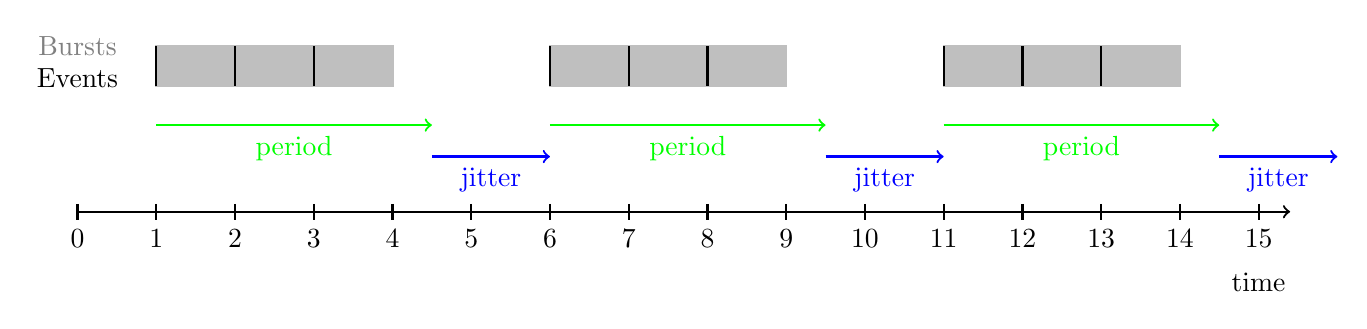
\begin{tikzpicture}[thick]
	% time axis
	\foreach \x in {0,...,15}
	\draw (\x,-4) -- (\x,-4.2) node[anchor=north] {\x};
	\draw[->] (0, -4.1) -- (15.4, -4.1);
	\node at(15, -5) {time};
	
	% bursts
	\node[gray] at (0, -2){Bursts};
	\draw [fill=lightgray, lightgray] (1, -2) rectangle (4,-2.5);
	\draw [fill=lightgray, lightgray] (6, -2) rectangle (9,-2.5);
	\draw [fill=lightgray, lightgray] (11, -2) rectangle (14,-2.5);
%	\draw [fill=lightgray, lightgray] (16, -2) rectangle (19,-2.5);
	% events
	\node at (0, -2.4){Events};
	%\node at (0, -2.15){events};
	\foreach \x in {1, 6, 11}
	{
		% events
		\draw[-] (\x, -2) -- (\x, -2.5);
		\draw[-] (\x+1, -2) -- (\x+1, -2.5);
		\draw[-] (\x+2, -2) -- (\x+2, -2.5);
		% periods
		\draw[->, green] (\x, -3) -- (\x+3.5, -3);
		\node[green] at (\x+1.75, -3.3){period};
		%jitters
		\draw[->, blue] (\x+3.5,-3.4) -- (\x+5, -3.4);
		\node[blue] at (\x+4.25, -3.7) {jitter};
	}
	\end{tikzpicture}
	\caption{BurstPatternEventTriggering \textit{patternPeriod} and \textit{patternJitter} \textbf{accumulating}}
	\label{fig:BurstPatternEventTriggering1}
\end{figure}
\begin{figure}
	\centering
	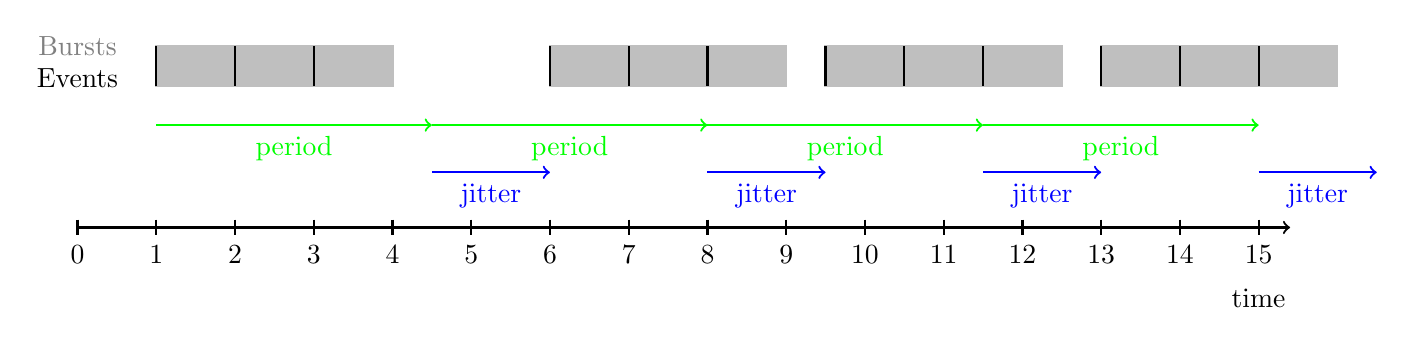
\begin{tikzpicture}[thick]
	% time axis
	\foreach \x in {0,...,15}
	\draw (\x,-4.2) -- (\x,-4.4) node[anchor=north] {\x};
	\draw[->] (0, -4.3) -- (15.4, -4.3);
	\node at(15, -5.2) {time};
	
	% bursts
	\node[gray] at (0, -2){Bursts};
	\draw [fill=lightgray, lightgray] (1, -2) rectangle (4,-2.5);
	\node at (0, -2.4){Events};
	
	%period 1
	\draw[->, green] (1, -3) -- (4.5, -3);
	\node[green] at (2.75, -3.3){period};
	
	% jitter 1
	\draw[->, blue] (4.5,-3.6) -- (6, -3.6);
	\node[blue] at (5.25, -3.9) {jitter};
	
	\foreach \y in {0, 1, 2}
	\draw[-] (1+\y, -2) -- (1+\y, -2.5);
	\foreach \x in {4.5, 8, 11.5}{
		%bursts	
		\draw [fill=lightgray, lightgray] (\x+1.5, -2) rectangle (\x+4.5,-2.5);
		% events
		\foreach \y in {0, 1, 2}
			\draw[-] (\x+\y+1.5, -2) -- (\x+\y+1.5, -2.5);
			
	}
	\foreach \x in {4.5, 8, 11.5}
	{
		% periods
		\draw[->, green] (\x, -3) -- (\x+3.5, -3);
		\node[green] at (\x+1.75, -3.3){period};
		% jitters
		\draw[->, blue] (\x+3.5,-3.6) -- (\x+5, -3.6);
		\node[blue] at (\x+4.25, -3.9) {jitter};
		
	}

	
	\end{tikzpicture}
	\caption{BurstPatternEventTriggering \textit{patternPeriod} and \textit{patternJitter} \textbf{non-accumulating}}
	\label{fig:BurstPatternEventTriggering2}
\end{figure}

The combination of $patternPeriod$ and $patternJitter$ can be interpreted in an accumulating way, as seen in figure~\ref{fig:BurstPatternEventTriggering1}, or in a non-accumulating way, as seen in figure~\ref{fig:BurstPatternEventTriggering2}. In the accumulating interpretation, the reference for the periodic occurrences is only the start point of the previous burst. In the non-accumulating way, there is a global reference point for the periodic repetitions.

With the definition of $patternPeriod$ (''time distance between the beginnings of subsequent repetitions of the given burst pattern''\cite{TIMEX}), you would think that the accumulating variant is meant. Against that, the period attribute in the \textit{PeriodicEventTriggering} constraint is defined as ''distance between subsequent occurrences of the event''\cite{TIMEX} in the text. Hence it is also understandable the accumulating way. However, there is the formal definition

\begin{math}
\exists t_{reference}\forall t_n: t_{reference}+(n+1)*period\leq t_n\leq t_{reference}+(n-1)*period+jitter,
\end{math}

where $t_n$ is the time of the $n$-th event and $t_{reference}$ is a reference point from which the periodic pattern starts, so the $PeriodicEventTriggering$ constraint is meant to be understood in the non-accumulating way. It remains unclear in which way the $BurstPatternEventTriggering$ is meant to be understood.

Another problem with the AUTOSAR Timing Extensions is that they were made for design purposes. Monitoring them can be difficult, as a monitor may need time and memory resources, which continuously grow with every input event. This makes online monitoring unsuitable in nearly all scenarios (more on monitorability in chapter~\ref{chapter-monitorability}). As an example, we will use the \textit{BurstPatternEventTriggering} again. This time we use the attributes
\begin{itemize}
	\item
	$maxNumberOfOccurrences = INT\_MAX$\textcolor{gray}{or any significant large number}
	\item
	$minNumberOfOccurrences = 1$
	\item
	$minimumInterArrivalTime = 0$
	\item
	$patternLength = 3$
	\item
	\textcolor{gray}{$patternPeriod$} \textcolor{gray}{unused}
	\item
	\textcolor{gray}{$patternJitter$} \textcolor{gray}{unused}
\end{itemize}

Figure~\ref{fig:BurstPatternEventTriggering3} shows the application of the \emph{BurstPatternEventTriggering} constraint with the given parameters on a stream with events at the timestamps 3, 3.5, 4, 4.5. The development of possible burst clusters with ongoing time is visualized. The gray bars show the range in which the burst cluster can lay. The black lines show where they definitely are. In timestamp 3, with only one event so far, only one burst has to be considered and it can lay between timestamp 0 and 6. The only limitation is that it must include timestamp 3 with the event at that point. In Timestamp 3.5, there are two events (at 3 and 3.5) so far, and there are two possibilities for burst placements. The first possibility is with only one burst with both events in it, and the second possibility, where the events are in different bursts. The third graphic shows the trace in timestamp 4 with three different events so far (3, 3.5, 4) and three different possibilities for burst placements to consider. One possible burst contains all three events, the second possibility has one burst with the event at timestamp 3 and one burst with the events at 3.5 and 4 and the third possibility has one Burst with the events at 3 and 3.5 and one burst with the event at 4. The possible bursts in graphic 4 are analog to the third graphic, one possibility with one burst containing all 4 events and 3 possibilities with the first burst containing the first event, the first and second event or the first, the second and the third event and the second burst containing the remaining events. Because the minimal distance between subsequent events is not specified, an arbitrarily large number of events can be placed in any interval with the length $patternLenth$.\\
In this example, we see that it is possible to create an unlimited number of possibilities for burst placements within one burst length when the \textit{minimumInterArrivalTime}-attribute is 0, which results in infeasible resource consumption because unlimited memory and time is needed to check the constraint in following events. Therefore, online monitoring of this constraint is unsuitable in most cases.

\begin{figure}
	\centering
	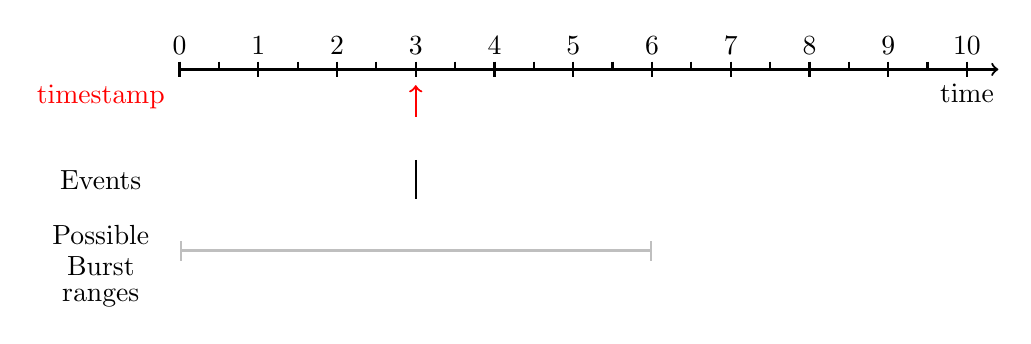
\begin{tikzpicture}[thick]
	%time axis
	\foreach \x in {0,...,10}
	{
		\draw (\x,0) -- (\x,-0.2);
		\node at (0+\x, 0.2) {\x};
	}
	\foreach \x in {0,...,9}
	\draw (\x+0.5,0) -- (\x+0.5,-0.1);
	\draw[->] (0, -0.1) -- (10.4, -0.1);
	\node at(10, -0.4) {time};
	
	\node[red] at(-1, -0.45) {timestamp};
	%watched time
	\draw[->, red] (3, -0.7)--(3, -0.3);
	
	\node at (-1, -1.5) {Events};
	\draw[-] (3, -1.25) -- (3, -1.75);
	
	\node at (-1, -2.2) {Possible};
	\node at (-1, -2.6) {Burst};
	\node at (-1, -3) {ranges};
	
	%Burst range
	\draw[|-|, lightgray] (0, -2.4) -- (6, -2.4);
	\end{tikzpicture}
	
	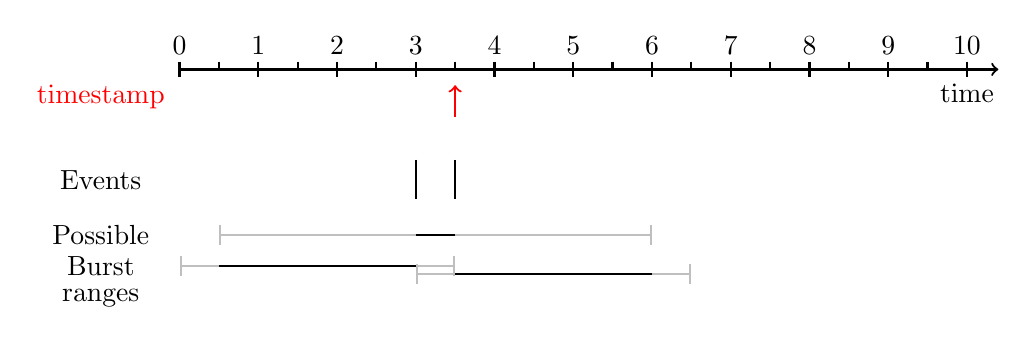
\begin{tikzpicture}[thick]
	%time axis
	\foreach \x in {0,...,10}
	{
		\draw (\x,0) -- (\x,-0.2);
		\node at (0+\x, 0.2) {\x};
	}
	\foreach \x in {0,...,9}
	\draw (\x+0.5,0) -- (\x+0.5,-0.1);
	\draw[->] (0, -0.1) -- (10.4, -0.1);
	\node at(10, -0.4) {time};
	
	\node[red] at(-1, -0.45) {timestamp};
	%watched time
	\draw[->, red] (3.5, -0.7)--(3.5, -0.3);
	
	\node at (-1, -1.5) {Events};
	\draw[-] (3, -1.25) -- (3, -1.75);
	\draw[-] (3.5, -1.25) -- (3.5, -1.75);
	
	\node at (-1, -2.2) {Possible};
	\node at (-1, -2.6) {Burst};
	\node at (-1, -3) {ranges};
	
	%Burst range 1
	\draw[|-|, lightgray] (0.5, -2.2) -- (6, -2.2);
	\draw[-] (3, -2.2) -- (3.5, -2.2);
	% Burst range 2
	\draw[|-|, lightgray] (0, -2.6) -- (3.5, -2.6);
	\draw[-] (0.5, -2.6) -- (3, -2.6);
	\draw[|-|, lightgray] (3, -2.7) -- (6.5, -2.7);
	\draw[-] (3.5, -2.7) -- (6, -2.7);
	\end{tikzpicture}
	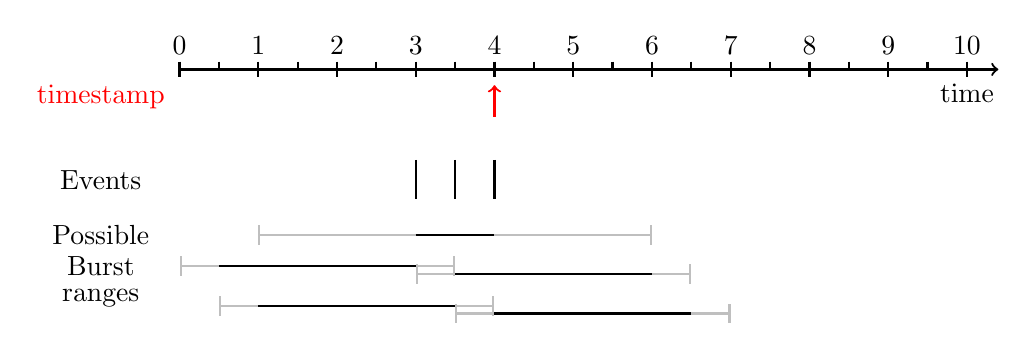
\begin{tikzpicture}[thick]
	%time axis
	\foreach \x in {0,...,10}
	{
		\draw (\x,0) -- (\x,-0.2);
		\node at (0+\x, 0.2) {\x};
	}
	\foreach \x in {0,...,9}
	\draw (\x+0.5,0) -- (\x+0.5,-0.1);
	\draw[->] (0, -0.1) -- (10.4, -0.1);
	\node at(10, -0.4) {time};
	
	\node[red] at(-1, -0.45) {timestamp};
	%watched time
	\draw[->, red] (4, -0.7)--(4, -0.3);
	
	\node at (-1, -1.5) {Events};
	\draw[-] (3, -1.25) -- (3, -1.75);
	\draw[-] (3.5, -1.25) -- (3.5, -1.75);
	\draw[-] (4, -1.25) -- (4, -1.75);
	
	\node at (-1, -2.2) {Possible};
	\node at (-1, -2.6) {Burst};
	\node at (-1, -3) {ranges};
	
	%Burst ranges poss. 1
	\draw[|-|, lightgray] (1, -2.2) -- (6, -2.2);
	\draw[-] (3, -2.2) -- (4, -2.2);
	% Burst ranges poss. 3 2.6,2.7
	\draw[|-|, lightgray] (0, -2.6) -- (3.5, -2.6);
	\draw[-] (0.5, -2.6) -- (3, -2.6);
	\draw[|-|, lightgray] (3, -2.7) -- (6.5, -2.7);
	\draw[-] (3.5, -2.7) -- (6, -2.7);
	% Burst ranges poss. 2
	\draw[|-|, lightgray] (0.5, -3.1) -- (4, -3.1);
	\draw[-] (1, -3.1) -- (3.5, -3.1);
	\draw[|-|, lightgray] (3.5, -3.2) -- (7, -3.2);
	\draw[-] (4, -3.2) -- (6.5, -3.2);
	\end{tikzpicture}
	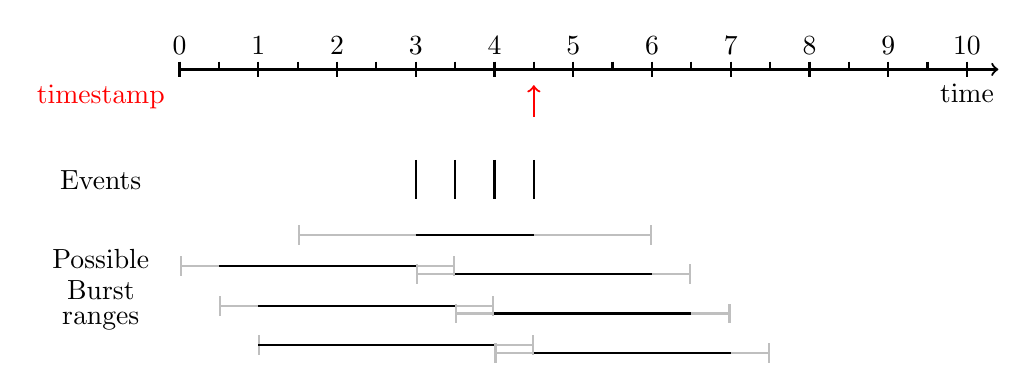
\begin{tikzpicture}[thick]
	%time axis
	\foreach \x in {0,...,10}
	{
		\draw (\x,0) -- (\x,-0.2);
		\node at (0+\x, 0.2) {\x};
	}
	\foreach \x in {0,...,9}
	\draw (\x+0.5,0) -- (\x+0.5,-0.1);
	\draw[->] (0, -0.1) -- (10.4, -0.1);
	\node at(10, -0.4) {time};
	
	\node[red] at(-1, -0.45) {timestamp};
	%watched time
	\draw[->, red] (4.5, -0.7)--(4.5, -0.3);
	
	\node at (-1, -1.5) {Events};
	\draw[-] (3, -1.25) -- (3, -1.75);
	\draw[-] (3.5, -1.25) -- (3.5, -1.75);
	\draw[-] (4, -1.25) -- (4, -1.75);
	\draw[-] (4.5, -1.25) -- (4.5, -1.75);
	
	\node at (-1, -2.5) {Possible};
	\node at (-1, -2.9) {Burst};
	\node at (-1, -3.3) {ranges};
	
	%Burst ranges poss. 1
	\draw[|-|, lightgray] (1.5, -2.2) -- (6, -2.2);
	\draw[-] (3, -2.2) -- (4.5, -2.2);
	% Burst ranges poss. 2
	\draw[|-|, lightgray] (0, -2.6) -- (3.5, -2.6);
	\draw[-] (0.5, -2.6) -- (3, -2.6);
	\draw[|-|, lightgray] (3, -2.7) -- (6.5, -2.7);
	\draw[-] (3.5, -2.7) -- (6, -2.7);
	% Burst ranges poss. 3
	\draw[|-|, lightgray] (0.5, -3.1) -- (4, -3.1);
	\draw[-] (1, -3.1) -- (3.5, -3.1);
	\draw[|-|, lightgray] (3.5, -3.2) -- (7, -3.2);
	\draw[-] (4, -3.2) -- (6.5, -3.2);
	% Burst ranges poss. 4
	\draw[|-|, lightgray] (1, -3.6) -- (4.5, -3.6);
	\draw[-] (1, -3.6) -- (4, -3.6);
	\draw[|-|, lightgray] (4, -3.7) -- (7.5, -3.7);
	\draw[-] (4.5, -3.7) -- (7, -3.7);
	\end{tikzpicture}
	\caption{BurstPatternEventTriggering Possible bursts, \textcolor{red}{$\uparrow$} shows the current time}
	\label{fig:BurstPatternEventTriggering3}
	
%TODO weiteres Beispiel für unsaubere Definition von AUTOSAR-> falsches Beispiel für file:///home/hendrik/Documents/Uni/Semester8/Quellen%20Bachelorarbeit/AutoSar%20TimEx/MethodologyAndTemplates/AUTOSAR_TPS_TimingExtensions.pdf
\end{figure}

\newpage

\section{Timing Augmented Description Language\cite{TIMMO2USE}}
	As timing extension to EAST-ADL(\textbf{E}lectronics \textbf{A}rchitecture and \textbf{S}oftware \textbf{T}echnology-\textbf{A}rchitecture \textbf{D}escription \textbf{L}anguage), the TIMMO (\textbf{Tim}ing \textbf{Mo}del) project, and its successor, TIMMO2USE, were initiated. A part of this project was the \textbf{T}iming \textbf{A}ugmented \textbf{D}escription \textbf{L}anguage V2 (TADL2), were created. TADL2 has similar goals as the AUTOSAR Timing Extensions, but the definitions are written in a more formalized fashion. While the definitions of the AUTOSAR Timing Extensions are only textually described often, the TADL2 definitions are defined more formally. They offer a formal definition of each constraint in the timing constraint logic TiCL \cite{TIMMO2USE}. EAST-ADL is much less used in the automotive industry, but the EAST-ADL Timing Constraints are partly compatible with the AUTOSAR Timing Extensions, as they are sub- or supersets of each other. Many of the AUTOSAR Timing Extensions can be defined via a combination of TADL2 Constraints, as explained in section~\ref{comparisonConstraints}.\\
	The timing constraints are defined on events or event chains, similar to the AUTOSAR Timing Extensions. In TADL2, all events of an event chain have a color attribute, which shows the logical connection of associated events. This attribute is defined as an abstract and possibly infinite datatype. The only restriction is that an equality test on these color values must be defined. TADL2 offers 18 timing constraints, which will be briefly explained in the following.
	\begin{itemize}
		\item
			The \textbf{StrongDelayConstraint} defines the minimal and maximal time distance of the events from two event sets (\emph{source} and \emph{target}).
		\item
			The \textbf{DelayConstraint} is a less strict variant of the \textbf{StrongDelayConstraint} because it allows additional events in the \emph{target} events.
		\item
			The \textbf{RepeatConstraint}, \textbf{RepetitionConstraint}, \textbf{PeriodicConstraint}, \textbf{SporadicConstraint} and \textbf{ArbitraryConstraint} describe the time distance between subsequent events, whereby they have small semantic differences. An exact distinction between these constraints will be given in section~\ref{tadl2Constraints}.
		\item
			The \textbf{SynchronizationConstraint} and \textbf{StrongSynchronizationConstraint} define groups of event sets, whose events occur in common time intervals. The SynchronizationConstraint allows more than one event of each group per interval, while the StrongSynchronizationConstraint does not.
		\item
			The \textbf{ExecutionTimeConstraint} sets a minimum and a maximum for the runtime of a task, not counting interruptions in the execution.
		\item
			The \textbf{OrderConstraint} defines that the $n^{th}$ event of one event set must occur before or at the $n^{th}$ event of a second event set.
		\item
			The \textbf{ComparisonConstraint} is used to describe ordering relations of timestamps.
		\item
			The \textbf{PatternConstraint} defines the time distance between periodic points in time and several events.
		\item
			The \textbf{BurstConstraint} regulates the maximum number of events in time intervals of a specific length.
		\item
			The \textbf{ReactionConstraint} describes the minimal and maximal time a response event must occur after the associated stimulus event. Additional response events are allowed, additional stimulus events are not.
		\item
			The \textbf{AgeConstraint} is similar to the ReactionConstraint, but it is defined the other way around. Therefore, it describes the minimal and maximal time a stimulus event must occur before the associated response event.  Additional stimulus events are allowed, additional response events are not.
		\item
			The \textbf{OutputSynchronizationConstraint} is used to describe groups of event chains, which all have the same response events. The response events of the event chain must occur in common time intervals, like in the SynchronizationConstraint. In the \textbf{InputSynchronizationConstraint}, the roles of the stimulus and response events are swapped.			
	\end{itemize}
	
\subsection{Parenthesis - Simple and Flexible Timing Constraint Logic}
	The formal definitions of the TADL2 timing constraint are written in \emph{Timing Constraint Logic} (short: \emph{TiCL}), which was developed as part of the TIMMO-2-USE project. TiCL was formally introduced in \cite{TiCL}. For better understanding, the key aspects of this paper will be explained in the following.\\
	The main goal of TiCL is to be formal and expandable and offering the possibility of defining finite and infinite behaviors of events. In TiCL, only points in time in which events occur are considered. Therefore every event only consists of a real number as a timestamp, without the possibility of adding a data value. There are seven syntactic categories in TiCL.
	\begin{align*}
		\mathbb{R} &\text{(arithmetic constants)}\\
		Avar &\text{(arithmetic variables)}\\
		AExp &\text{(arithmetic expressions)}\\[10pt]
		%\vspace{1cm}
		Svar &\text{(set variables)}\\
		SExp &\text{(set expressions)}\\[10pt]
		%\vspace{1cm}
		TVar &\text{(time variables)}\\
		CExp &\text{(constraint expressions)}
	\end{align*}
	Arithmetic expressions can be defined as arithmetic constants, as arithmetic variables, as an application of $+,-,*,/$ on arithmetic expressions, as an application of the cardinality operator on a set ($|E|$, $E\in SExp$) or as measure $\lambda(E)$ ($E\in SExp$). $\lambda(E)$ is defined as the Lebesgue measure, which is figuratively speaking, the length of all continuous intervals of $E$. In figure~\ref{fig:TiCLMeasureExample}, an example of the measure operator $\lambda$ is visualized. The set $E$ contains all Events between the timestamps $1$ and $9$. The set $F$ contains the events at the timestamps between 2 and 4 and 6 and 7. Therefore $E\setminus F$ contains the events at the timestamps $\{1, 1.5, 4.5, 5, 5.5, 7.5, 8, 8.5, 9\}$.
	$E$ consists of one continuous interval from timestamp 1 to 9 with the length of 8, $F$ consists of two continuous intervals from 2 to 4 with the length of 2 and from 6 to 7 with the length of 1, therefore $\lambda(F)=3$. $E\setminus F$ consists of three continuous intervals, the first from 1 to 1.5 (length = 0.5), the second from 4.5 to 5.5 (length = 1) and the last from 7.5 to 9 (length = 1.5). Consequently, the total length of the continuous intervals of $E\setminus F$ is 3.\\
	% TODO richtig? vgl. executionTimeConstraint-> ja richtig. [x..y] beschreibt Interval mit allen mögl. Zeitpunkten dadrin.
	\begin{figure}
		\centering
		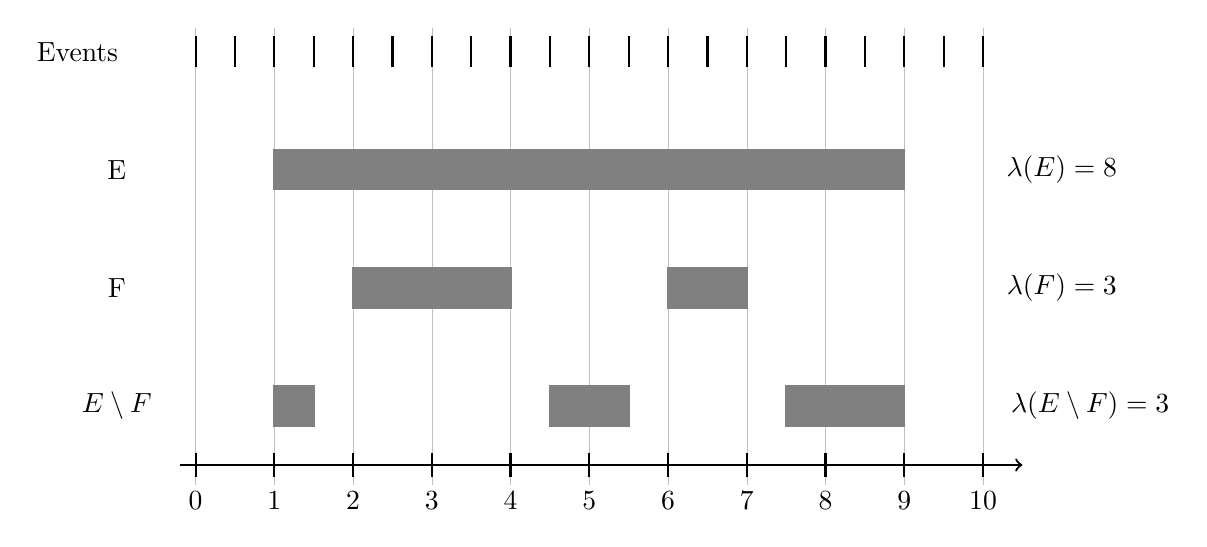
\begin{tikzpicture}[thick]
			\foreach \x in {0,...,10}
			{
				\draw[very thin, lightgray](\x, 1.8) -- (\x, -4);
				
				\draw (\x,-3.6) -- (\x,-3.9);
				\node at (0+\x, -4.2) {\x};
			}
			\draw[->] (-0.2, -3.75) -- (10.5, -3.75);
			
			\node at (-1,  0) {E};
			\draw [fill=gray,gray] (1,0.25) rectangle (9,-0.25); 
			
			\node at (-1, -1.5) {F};
			\draw [fill=gray,gray] (2,-1.25) rectangle (4,-1.75); 
			\draw [fill=gray,gray] (6,-1.25) rectangle (7,-1.75);
			
			\node at (-1, -3) {$E \setminus F$};
			\draw [fill=gray,gray] (1,-2.75) rectangle (1.5,-3.25); 
			\draw [fill=gray,gray] (4.5,-2.75) rectangle (5.5,-3.25);
			\draw [fill=gray,gray] (7.5,-2.75) rectangle (9,-3.25);
			
			\node at (11, 0) {$\lambda(E) = 8$};
			\node at (11, -1.5) {$\lambda(F) = 3$};
			\node at (11.36, -3) {$\lambda(E\setminus F) = 3$};
			
			\node at (-1.5, 1.5){Events};
			\foreach \x in {0, 0.5, ...,10}
			\draw (\x, 1.7) -- (\x, 1.3);
		\end{tikzpicture}
		\caption{Graphical example of $\lambda(E), \lambda(F)$ and $\lambda(E\setminus F)$}
		\label{fig:TiCLMeasureExample}
	\end{figure}
	Set expressions can be defined as set variables or as a set of time variables that fulfill a given constraint expression.\\
	Constraint expressions can be defined as an application of the $\leq$ operator on time or arithmetic expressions, the $\in$ operator on time variables and set expressions, the logical conjunction ($\land$) on constraint expressions, the negation of constraint expressions and the $\forall$-Quantifier on arithmetic, set and time variables over a constraint expression.\\
	As an extension to this definition, well known syntactic abbreviations like $true\equiv 0\leq 1$ or the $\exists$-quantifier are defined. There are also some TiCL-specific syntactic abbreviations, such as interval constructors, which will be defined and explained in the following.\\
	Let $x, y\in Tvar$ and $E, F\in SExp$.
	\begin{itemize}
		\item
			The interval constructor $[x<]$($[x\leq]$) is defined as $\{y: x < y\}$($\{y: x \leq y\}$), therefore the interval contains all points in time laying behind of $x$ (including $x$).
		\item
			$[\leq x]$($[< x]$) is defined as complement of $[x<]$($[x\leq]$) and contains all timestamps laying before $x$.
		\item
			$[x..y]$ is defined as $[x\leq]\cap[<y]$, so all points of time after $x$ and before $y$, including $x$ but not $y$, are part of this interval.
		\item
			$[E \leq]$ is defined as $\{y : \exists x \in E : x \leq y\}$, this interval contains all points in time at and after the first timestamp in $E$.
		\item
			$[E<]$ is equal to $\{y : \forall x \in E : x < y\}$, therefore it defines the interval containing all timestamps after the latest point of time in $E$. Please note the use of $\forall$ instead $\exists$ in the definition.
		\item
			$[\leq E]$ ($[< E]$) is defined as $[E<]^C$ ($[E\leq]^C$), analogous to the operators on time variables.
		\item
			$[E]$ is equal to $[E\leq]\cap[\leq E]$. It defines the time interval between the first and last element of $E$, including these points in time.
		\item
			$E_{x<}$($E_{<x}$) is defined as $E\cap [x<]$($E\cap [<x]$). This operators filters the timestamps in $E$ so that only the points in time before (after) $x$ remain.
		\item
			$[x..E]$ equals $[x\leq]\cap[<(E_{x<})]$. The interval begins at $x$ and ends right before the first element of $E$ after $x$.
		\item
			$[E..F]$ is defined as $\{x:\exists y\in E:x\in[y..F]\}$ and describes the intervals, where the previous operator is applied on every element of $E$.
		\item
			$E(i)$ is $i^{th}$ timestamp in $E$, starting at zero.
		\item
				$E\leq F$ describes, that $E$ is a sub sequence of $F$, which means that between the earliest and latest element in $E$ all elements of $F$ are in $E$.
	\end{itemize}

	

	% TODO x-y/y-x ???
	% TODO X\leq Y -> X is subsequence of Y needed???
\subsection{TADL2-Timing Constraints}
	\label{tadl2Constraints}
	For a better understanding of the following chapters, the TADL Constraints will be presented next. As abbreviation and unification, all timing expressions are defined over set $\mathbb{T}$, which is understood as real numbers but expanded with $\infty$ and $-\infty$ in this chapter. Other value ranges for time expressions are possible and will be used later in this thesis.\\
	We define an event as a time value, possibly combined with a data value. The range of the data values is arbitrary. Infinite data types are possible, as well as empty data types when only the point in time is relevant for the constraint. All TADL constraints are defined with attributes, which can be events, timing or arithmetic expressions or sets of them. Also, \emph{EventChains} can be used as attributes. An \emph{EventChain} consists of two sets of events (\emph{stimulus} and \emph{response}),  which are causally related. All events in an \emph{EventChain} must have a color value in their data field. This color possibly has an infinite type and an equality check on the datatype of the color must be defined. It is used to check which events of an \emph{EventChain} are directly related.
	\subsubsection{DelayConstraint}
		The \emph{DelayConstraint} has four attributes
		\begin{align*}
			\emph{source} & \hspace{.5cm}\text{event set}\\
			\emph{target} & \hspace{.5cm}\text{event set}\\
			\emph{lower}  & \hspace{.5cm}\text{$\mathbb{T}$ (time expression)}\\
			\emph{upper}  & \hspace{.5cm}\text{$\mathbb{T}$}
		\end{align*}
		and is defined as\\[10pt]
		\begin{math}
			DelayConstraint ( source, target, lower, upper )\\
			\Leftrightarrow \forall x\in source:\exists y\in target: lower\leq y-x\leq upper.
		\end{math}\\[10pt]
		For all events $x$ in \emph{source}, there must be an event $y$ in \emph{target}, so that the time distance between $x$ and $y$ is between \emph{lower} and \emph{upper}. Note that \emph{lower} and \emph{upper} can have negative values and that additional events in \emph{target} without an associated \emph{source} event are allowed.\\
		Figure~\ref{fig:delayConstraintExample} shows a visualized example of the \emph{DelayConstraint} with the attributes $lower=2$, $upper=3$, $source=\{1, 5, 6\}$ and $target=\{2, 3.5, 5, 7, 8.2, 9\}$. The first element of source at timestamp 1 results in a required event in target between the timestamp 3 and 4 that is fulfilled by the event at 3.5. The second event of source requires a target event between 7 and 8, fulfilled by the event at 7. The last event of source is satisfied by the target event at 8.2 and 9.
		\begin{figure}
			\centering
			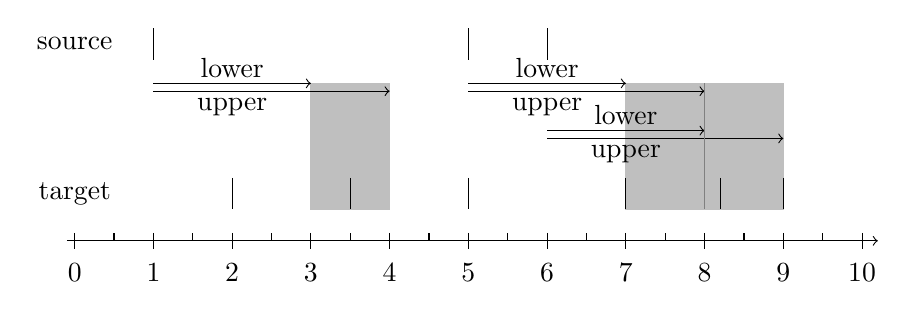
\begin{tikzpicture}
				% source events
				\node[] at (0,-0.2){source};
				\draw (1, 0) -- (1, -0.4);
				\draw (5, 0) -- (5, -0.4);
				\draw (6, 0) -- (6, -0.4);
				
				% upper/lower 1
				\draw [fill=lightgray, lightgray] (3, -0.7) rectangle (4,-2.3);
				\node at (2, -0.5){lower};
				\node at (2, -1){upper};
				\draw[->] (1,-0.7) -- (3, -0.7);
				\draw[->] (1, -0.8) -- (4, -0.8);
				
				
				% upper/lower 2
				\draw [fill=lightgray, lightgray] (7, -0.7) rectangle (8,-2.3);
				\node at (6, -0.5){lower};
				\node at (6, -1){upper};
				\draw[->] (5,-0.7) -- (7, -0.7);
				\draw[->] (5, -0.8) -- (8, -0.8);
				
				% upper/lower 3
				\draw [fill=lightgray, lightgray] (8, -0.7) rectangle (9,-2.3);
				\node at (7, -1.1){lower};
				\node at (7, -1.6){upper};
				\draw[->] (6,-1.3) -- (8, -1.3);
				\draw[->] (6, -1.4) -- (9, -1.4);
				% target events
				\node[] at (0,-2.1){target};
				\draw (2, -1.9) -- (2, -2.3);
				\draw (3.5, -1.9) -- (3.5, -2.3);
				\draw (5, -1.9) -- (5, -2.3);
				\draw (7, -1.9) -- (7, -2.3);
				\draw (8.2, -1.9) -- (8.2, -2.3);
				\draw (9, -1.9) -- (9, -2.3);
				
				\foreach \x in {0, 1, ..., 10}{
					\draw (\x, -2.6) -- (\x, -2.8);
					\node at(\x, -3.1) {\x};
				}
			
				\foreach \x in {0.5, 1.5, ..., 9.5}{
					\draw (\x, -2.7) -- (\x, -2.6);
				}
				\draw[->] (-0.1, -2.7) -- (10.2, -2.7);
				
				\draw[gray] (8,-0.7)--(8,-2.3);
					
			\end{tikzpicture}
			\caption{Example DelayConstraint - $lower = 2$, $upper = 3$}
			\label{fig:delayConstraintExample}
		\end{figure}
	\subsubsection{StrongDelayConstraint}
		The \emph{StrongDelayConstraint} has four attributes
		\begin{align*}
			\emph{source} & \hspace{.5cm}\text{event set}\\
			\emph{target} & \hspace{.5cm}\text{event set}\\
			\emph{lower}  & \hspace{.5cm}\text{$\mathbb{T}$}\\
			\emph{upper}  & \hspace{.5cm}\text{$\mathbb{T}$}
		\end{align*}
		and is defined as\\[10pt]
		\begin{math}
			StrongDelayConstraint( source, target, lower, upper )\\
			|source| = |target| \land\\
			\forall i: \forall x: x=source(i) \Rightarrow \exists y: y=target(i)\land lower\leq y-x\leq upper.
		\end{math}\\[10pt]
		The \emph{StrongDelayConstraint} is a stricter version of the \emph{DelayConstraint}, as it requires a bijective assignment between the source and target events. Therefore additional events in target without matching source event are not allowed. Figure~\ref{fig:StrongDelayConstraintExample} shows an example of the \emph{StrongDelayConstraint}. The example is the same as in the previous constraint, but without the additional target events at 2, 5 and 8.2.
 		\begin{figure}
			\centering
		 	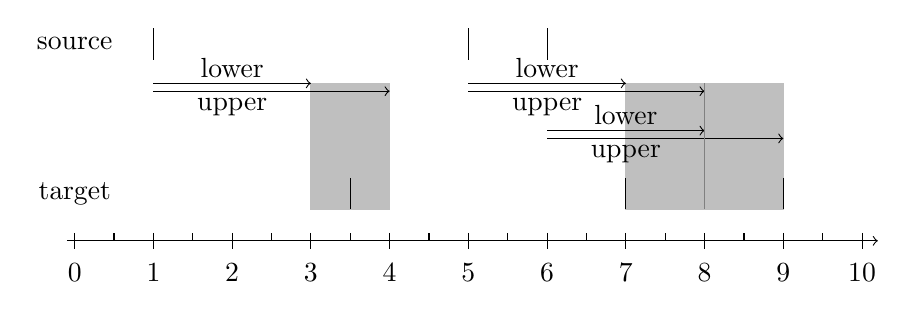
\begin{tikzpicture}
		 	% source events
		 	\node[] at (0,-0.2){source};
		 	\draw (1, 0) -- (1, -0.4);
		 	\draw (5, 0) -- (5, -0.4);
		 	\draw (6, 0) -- (6, -0.4);
		 	
		 	% upper/lower 1
		 	\draw [fill=lightgray, lightgray] (3, -0.7) rectangle (4,-2.3);
		 	\node at (2, -0.5){lower};
		 	\node at (2, -1){upper};
		 	\draw[->] (1,-0.7) -- (3, -0.7);
		 	\draw[->] (1, -0.8) -- (4, -0.8);
		 	
		 	
		 	% upper/lower 2
		 	\draw [fill=lightgray, lightgray] (7, -0.7) rectangle (8,-2.3);
		 	\node at (6, -0.5){lower};
		 	\node at (6, -1){upper};
		 	\draw[->] (5,-0.7) -- (7, -0.7);
		 	\draw[->] (5, -0.8) -- (8, -0.8);
		 	
		 	% upper/lower 3
		 	\draw [fill=lightgray, lightgray] (8, -0.7) rectangle (9,-2.3);
		 	\node at (7, -1.1){lower};
		 	\node at (7, -1.6){upper};
		 	\draw[->] (6,-1.3) -- (8, -1.3);
		 	\draw[->] (6, -1.4) -- (9, -1.4);
		 	% target events
		 	\node[] at (0,-2.1){target};
		 	\draw (3.5, -1.9) -- (3.5, -2.3);
		 	\draw (7, -1.9) -- (7, -2.3);
		 	\draw (9, -1.9) -- (9, -2.3);
		 	
			\foreach \x in {0, 1, ..., 10}{
				\draw (\x, -2.6) -- (\x, -2.8);
				\node at(\x, -3.1) {\x};
			}
		
			\foreach \x in {0.5, 1.5, ..., 9.5}{
				\draw (\x, -2.7) -- (\x, -2.6);
			}
			\draw[->] (-0.1, -2.7) -- (10.2, -2.7);
		 	
		 	\draw[gray] (8,-0.7)--(8,-2.3);
		 	\end{tikzpicture}
		 	\caption{Example StrongDelayConstraint - $lower = 2$, $upper = 3$}
		 	\label{fig:StrongDelayConstraintExample}
		 \end{figure}
	\subsubsection{RepeatConstraint}
		The \emph{RepeatConstraint} also has four attributes
		\begin{align*}
			\emph{event} & \hspace{.5cm}\text{event set}\\
			\emph{lower} & \hspace{.5cm}\text{$\mathbb{T}$}\\
			\emph{upper} & \hspace{.5cm}\text{$\mathbb{T}$}\\
			\emph{span}	 & \hspace{.5cm}\text{$integer$}\\
		\end{align*}
		and is defined as\\[10pt]
		\begin{math}
			RepeatConstraint ( event, lower, upper, span )\\
			\Leftrightarrow\forall X\leq event: |X|=span+1\Rightarrow lower \leq \lambda([X])\leq upper.
		\end{math}\\[10pt]
		As a reminder, the $\leq$-operator over two sets of events $A, B$ describes that $A$ is a subsequence of $B$, the $\lambda(A)$-function calculates the total length of all continuous intervals in $A$ and $[A]$ is the time interval between the oldest and newest event in $A$.\\ \\
		The definition of the \textit{RepeatConstraint} specifies that the length of each time interval containing $span+1$ subsequent events must be between $upper$ and $lower$.\\
		The idea behind this constraint is to define repeated occurrences of events, with the possibility of overlapping, specified by the \emph{span} attribute. After any event $x$, there are $span-1$ events and then the next event must be between $lower$ and $upper$ after $x$.\\
		Figure~\ref{fig:RepeatConstraintExample1} shows an example of the RepeatConstraint with the attributes $event=\{3,5,8,...\}$, $lower=upper=2$ and $span=1$. Because $lower$ is equal to $upper$ and $span$ is 1, the events follow a strictly periodic pattern after the first event. Figure~\ref{fig:RepeatConstraintExample2} shows a more complex example with events at $\{0, 2, 4, 7, 9, 11,...\}$, $lower=4$, $upper=5$ and $span=2$. The $span$-attribute is 2, so the time distances between all subsequent events with an even index are considered, as well as the distances between subsequent events with an uneven index. 
		
		\begin{figure}
			\centering
			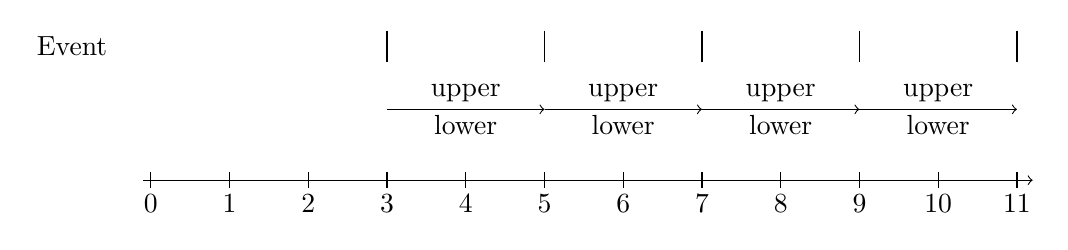
\begin{tikzpicture}
				% events
				\node at(-1 , 0.2){Event}; 
				\foreach \x in {3,5,...,9}{
					\draw (\x, 0.4) -- (\x, 0);
					\draw[->] (\x, -0.6) -- (\x+2, -0.6);
					\node at(\x+1, -0.8){lower};
					\node at(\x+1, -0.4){upper};
				}
				\draw (11, 0.4) -- (11, 0);
				% time axis
				\foreach \x in {0,...,11}{
					\draw (\x, -1.4) -- (\x, -1.6);
					\node at(\x, -1.8){\x};
				}
				\draw[->] (-0.1, -1.5) -- (11.2, -1.5);
			\end{tikzpicture}
			\caption{Example RepeatConstraint - $lower = 2$, $upper = 2$, $span = 1$}
			\label{fig:RepeatConstraintExample1}
		\end{figure}
		\begin{figure}
			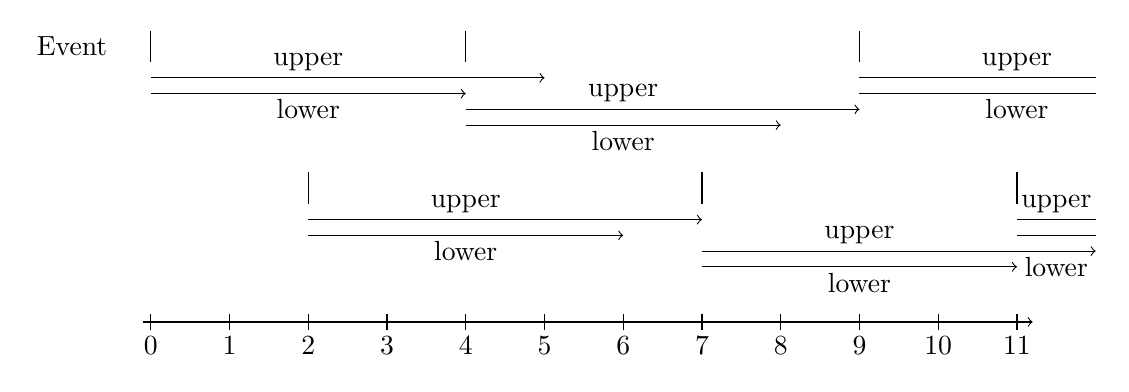
\begin{tikzpicture}
				\node at(-1, 0.2){Event};
				%eventreihe 1
				\foreach \x in {0, 4, 9} {
					\draw (\x,0) -- (\x, 0.4);
				}
				\foreach \x in {0} {
					\node at (\x+2, 0) {upper};
					\draw[->] (\x, -0.2) -- (\x+5, -0.2);
					\draw[->] (\x, -0.4) -- (\x+4, -0.4);
					\node at (\x+2, -0.6) {lower};
				}
				\foreach \x in {9} {
					\node at (\x+2, 0) {upper};
					\draw[-] (\x, -0.2) -- (12, -0.2);
					\draw[-] (\x, -0.4) -- (12, -0.4);
					\node at (\x+2, -0.6) {lower};
				}
				\foreach \x in {4} {
					\node at (\x+2, -0.4) {upper};
					\draw[->] (\x, -0.6) -- (\x+5, -0.6);
					\draw[->] (\x, -0.8) -- (\x+4, -0.8);
					\node at (\x+2, -1) {lower};
				}
				%eventreihe 2
				\foreach \x in {2, 7, 11} {
					\draw (\x,-1.4) -- (\x, -1.8);
				}
				\foreach \x in {2} {
					\node at (\x+2, -1.8) {upper};
					\draw[->] (\x, -2) -- (\x+5, -2);
					\draw[->] (\x, -2.2) -- (\x+4, -2.2);
					\node at (\x+2, -2.4) {lower};
				}
				\foreach \x in {11} {
					\node at (\x+0.5, -1.8) {upper};
					\draw[-] (\x, -2) -- (12, -2);
					\draw[-] (\x, -2.2) -- (12, -2.2);
					\node at (\x+0.5, -2.6) {lower};
				}
				\foreach \x in {7} {
					\node at (\x+2, -2.2) {upper};
					\draw[->] (\x, -2.4) -- (\x+5, -2.4);
					\draw[->] (\x, -2.6) -- (\x+4, -2.6);
					\node at (\x+2, -2.8) {lower};
				}
				%time axis
				\foreach \y in {-3.2}{
					\foreach \x in {0,...,11}{
						\draw (\x, \y) -- (\x, \y-0.2);
						\node at(\x, \y-0.4){\x};
					}
					\draw[->] (-0.1, \y-0.1) -- (11.2, \y-0.1);
				}
			\end{tikzpicture}
			\caption{Example RepeatConstraint - $lower = 4$, $upper = 5$, $span = 2$}
			\label{fig:RepeatConstraintExample2}
		\end{figure}
	
	\subsubsection{RepetitionConstraint}
		The \emph{RepetitionConstraint} has five attributes
		\begin{align*}
			\emph{event} & \hspace{.5cm}\text{event set}\\
			\emph{lower} & \hspace{.5cm}\text{$\mathbb{T}$}\\
			\emph{upper} & \hspace{.5cm}\text{$\mathbb{T}$}\\
			\emph{span}	 & \hspace{.5cm}\text{$integer$}\\
			\emph{jitter}& \hspace{.5cm}\mathbb{T}
		\end{align*}
		and is defined via the \emph{RepeatConstraint} and the \emph{StrongDelayConstraint} as\\[10pt]
		\begin{math}
			RepetitionConstraint ( event, lower, upper, span, jitter )\\
			\Leftrightarrow
			\exists X: RepeatConstraint(X, lower, upper, span) \land \\
			\text{\hspace{1cm}}StrongDelayConstraint(X, event, 0, jitter)
		\end{math}\\[10pt]
		where $X$ is a set of arbitrary timestamps that follow the structure of the \emph{RepeatConstraint}(various(\emph{span}) loose periodic repetitions). The actual points in time of \emph{event} lay between the timestamps of $X$ and $jitter$ after that. For each point of time there is exactly one, corresponding timestamp in $X$.
		Figure~\ref{fig:RepetitionConstraintExample} shows an example of the \emph{RepetitionConstraint} with the attributes $event=\{0.5, 3.3, 4.7, 7.6, 9.9, ...\}$, $lower=4$, $upper=5$, $span=2$ and $jitter=1$. The shown timestamps of $X$ are only one possibility and may change due to later elements of $event$.
		
		\begin{figure}
			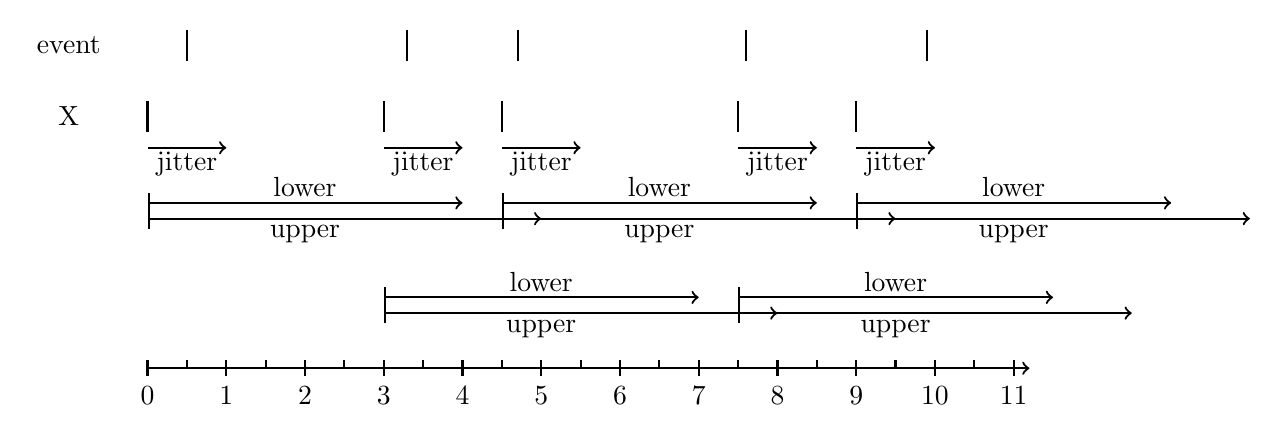
\begin{tikzpicture}[thick]
				% time axis
				\foreach \y in {-4}{
					\foreach \x in {0,...,11}
					\draw (\x,\y) -- (\x,\y-0.2) node[anchor=north] {\x};
					\foreach \x in {0.5,1.5,...,10.5}
					\draw (\x,\y) -- (\x,\y-0.1);
					\draw[->] (0,\y-0.1) -- (11.2, \y-0.1);
				}
			\node[] at (-1, 0) {event};
			\foreach \x in {0.5, 3.3, 4.7, 7.6, 9.9}
				\draw (\x, 0.2) -- (\x, -0.2);
			
			\node[] at (-1, -0.9) {X};
			\foreach \x in {0, 3, 4.5, 7.5, 9}{
				\draw (\x, -0.7) -- (\x, -1.1);
				\draw[->] (\x, -1.3) -- (\x+1, -1.3);
				\node at (\x+0.5, -1.5) {jitter};
			}
			\foreach \x in {0, 4.5, 9}{
				\node at (\x+2, -1.8) {lower};
				\draw[|->] (\x, -2) -- (\x+4, -2);
				\draw[|->] (\x, -2.2) -- (\x+5, -2.2);
				\node at (\x+2, -2.4) {upper};
			}
			\foreach \x in {3, 7.5}{
				\node at (\x+2, -3) {lower};
				\draw[|->] (\x, -3.2) -- (\x+4, -3.2);
				\draw[|->] (\x, -3.4) -- (\x+5, -3.4);
				\node at (\x+2, -3.6) {upper};
			}
			\end{tikzpicture}
			\caption{Example RepetitionConstraint - $lower = 4$, $upper = 5$, $span = 2$, $jitter=1$}
			\label{fig:RepetitionConstraintExample}
		\end{figure}
		
	
	\subsubsection{SynchronizationConstraint}
		The \emph{SynchronizationConstraint} has two attributes
		\begin{align*}
			\emph{event} & \hspace{.5cm}\text{set of event sets, $|event|\geq 2$}\\
			\emph{tolerance} & \hspace{.5cm}\mathbb{T}
		\end{align*}
		and is defined via the \emph{DelayConstraint} as\\[10pt]
		\begin{math}
			SynchronizationConstraint ( event_1, ..., event_n, tolerance )\\
			\Leftrightarrow\exists X: \forall i: DelayConstraint(X, event_i, 0, tolerance) \land\\
			\text{\hspace{1cm}}DelayConstraint(event_i, X, -tolerance, 0)
		\end{math}\\[10pt]
		$X$ is a set of timestamps, and there must be at least one timestamp between an element of $X$ and $tolerance$ after that in each set of \emph{event}. Also, there must be a matching element of $X$ for each element in any set of \emph{event}. \\
		In figure~\ref{fig:SynchronizationConstraintExample} is an example of the \emph{SynchronizationConstraint} with the attributes $event=\{\{0.5, 3, 7, 7.5\}, \{0.7, 2.5, 7.3, 7.8\}, \{1.2, 3.2, 3.3, 3.4, 7.6, 8.4\}\}$ and $tolerance = 1$. The first points in time of each element of event form the first cluster, the corresponding element of $X$ can be between $0.2$ and $0.5$. For simplification, only the latest possible value for the element of $X$ is shown, which is the first event of the synchronization cluster. In the second cluster of events, it can be seen that multiple timestamps from one element of $event$ can be associated with a single element of $X$. The third and fourth clusters show that overlapping is also possible.
		\begin{figure}			
			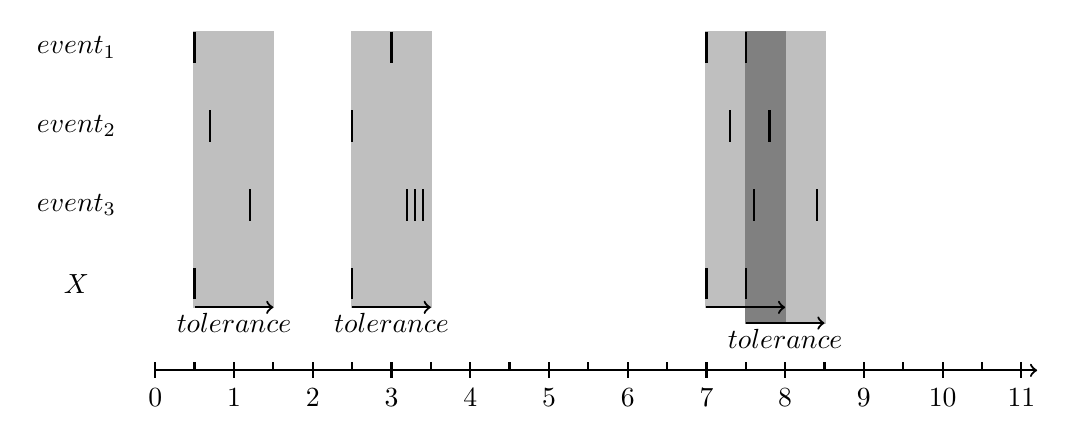
\begin{tikzpicture}[thick]
				% tolerance rectangles
				\foreach \x in {0.5, 2.5, 7}
					\draw [fill=lightgray, lightgray] (\x, 0.2) rectangle (\x+1, -3.3);
				\draw [fill=lightgray, lightgray] (7.5, 0.2) rectangle (8.5, -3.5);
				\draw [fill=gray, gray] (7.5, 0.2) rectangle (8, -3.5);
				% time axis
				\foreach \y in {-4}{
					\foreach \x in {0,...,11}
						\draw (\x,\y) -- (\x,\y-0.2) node[anchor=north] {\x};
					\foreach \x in {0.5,1.5,...,10.5}
						\draw (\x,\y) -- (\x,\y-0.1);
					\draw[->] (0,\y-0.1) -- (11.2, \y-0.1);
				}
				
				\node at (-1, 0){$event_1$};
				\foreach \x in {0.5, 3, 7, 7.5}
					\draw (\x, 0.2) -- (\x, -0.2);
				
				\node at (-1, -1){$event_2$};
				\foreach \x in {0.7, 2.5, 7.3, 7.8}
					\draw (\x, -0.8) -- (\x, -1.2);
				
				\node at (-1, -2){$event_3$};
				\foreach \x in {1.2, 3.2, 3.3, 3.4, 7.6, 8.4}
					\draw (\x, -1.8) -- (\x, -2.2);
					
				\node at (-1, -3){$X$};
				\foreach \x in {0.5, 2.5}{
					\draw (\x, -2.8) -- (\x, -3.2);
					\draw[->] (\x, -3.3) -- (\x+1, -3.3);
					\node at (\x+0.5, -3.5){$tolerance$};
				}
				\foreach \x in {7}{
					\draw (\x, -2.8) -- (\x, -3.2);
					\draw[->] (\x, -3.3) -- (\x+1, -3.3);
				}
				\foreach \x in {7.5}{
					\draw (\x, -2.8) -- (\x, -3.2);
					\draw[->] (\x, -3.5) -- (\x+1, -3.5);
					\node at (\x+0.5, -3.7){$tolerance$};
				}
					
			\end{tikzpicture}
			\caption{Example SynchronizationConstraint - $tolerance = 1$}
			\label{fig:SynchronizationConstraintExample}
		\end{figure}
		
		
		
	\subsubsection{StrongSynchronizationConstraint}
		The \emph{StrongSynchronizationConstraint} has the same two attributes as the \emph{SynchronizationConstraint}
		\begin{align*}
			\emph{event} & \hspace{.5cm}\text{set of event sets, $|event|\geq 2$}\\
			\emph{tolerance} & \hspace{.5cm}\mathbb{T}
		\end{align*}
		and is defined as\\[10pt]
		\begin{math}\\
			StrongSynchronizationConstraint ( event_1, …, event_n, tolerance )\\
			\Leftrightarrow\exists X: \forall i: StrongDelayConstraint(X, event_i, 0, tolerance)
		\end{math}\\[10pt]
		This constraint is a stricter variant of the \emph{SynchronizationConstraint}, as it requires a bijective assignment between the elements of $X$ to one element of each set of $event$. For every $x\in X$, only one corresponding timestamp per set in $event$ is allowed, as seen in figure~\ref{fig:StrongSynchronizationConstraintExample}, which shows the same example as the one for the \emph{SynchronizationConstraint}, but the excess time stamps at $3.2$ and $3.3$ have been removed.
			\begin{figure}			
				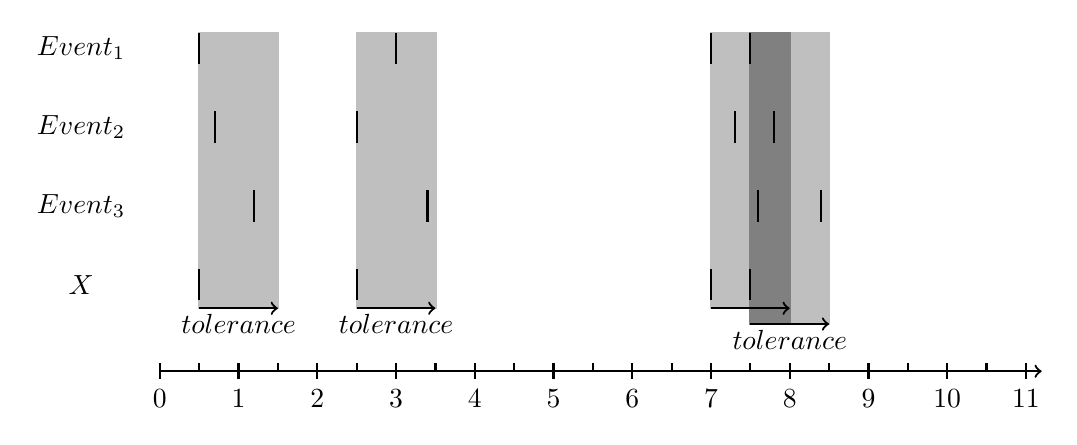
\begin{tikzpicture}[thick]
				% tolerance rectangles
				\foreach \x in {0.5, 2.5, 7}
				\draw [fill=lightgray, lightgray] (\x, 0.2) rectangle (\x+1, -3.3);
				\draw [fill=lightgray, lightgray] (7.5, 0.2) rectangle (8.5, -3.5);
				\draw [fill=gray, gray] (7.5, 0.2) rectangle (8, -3.5);
				% time axis
				\foreach \y in {-4}{
					\foreach \x in {0,...,11}
					\draw (\x,\y) -- (\x,\y-0.2) node[anchor=north] {\x};
					\foreach \x in {0.5,1.5,...,10.5}
					\draw (\x,\y) -- (\x,\y-0.1);
					\draw[->] (0,\y-0.1) -- (11.2, \y-0.1);
				}
				
				\node at (-1, 0){$Event_1$};
				\foreach \x in {0.5, 3, 7, 7.5}
				\draw (\x, 0.2) -- (\x, -0.2);
				
				\node at (-1, -1){$Event_2$};
				\foreach \x in {0.7, 2.5, 7.3, 7.8}
				\draw (\x, -0.8) -- (\x, -1.2);
				
				\node at (-1, -2){$Event_3$};
				\foreach \x in {1.2, 3.4, 7.6, 8.4}
				\draw (\x, -1.8) -- (\x, -2.2);
				
				\node at (-1, -3){$X$};
				\foreach \x in {0.5, 2.5}{
					\draw (\x, -2.8) -- (\x, -3.2);
					\draw[->] (\x, -3.3) -- (\x+1, -3.3);
					\node at (\x+0.5, -3.5){$tolerance$};
				}
				\foreach \x in {7}{
					\draw (\x, -2.8) -- (\x, -3.2);
					\draw[->] (\x, -3.3) -- (\x+1, -3.3);
				}
				\foreach \x in {7.5}{
					\draw (\x, -2.8) -- (\x, -3.2);
					\draw[->] (\x, -3.5) -- (\x+1, -3.5);
					\node at (\x+0.5, -3.7){$tolerance$};
				}
			
			\end{tikzpicture}
			\caption{Example StrongSynchronizationConstraint - $tolerance = 1$}
			\label{fig:StrongSynchronizationConstraintExample}
		\end{figure}
		
		
	\subsubsection{ExecutionTimeConstraint}
		The \emph{ExecutionTimeConstraints} takes six attributes
		\begin{align*}
			\emph{start} & \hspace{.5cm}\text{set of events}\\
			\emph{stop} & \hspace{.5cm}\text{set of events}\\
			\emph{preempt} & \hspace{.5cm}\text{set of events}\\
			\emph{resume} & \hspace{.5cm}\text{set of events}\\
			\emph{lower} & \hspace{.5cm}\mathbb{T}\\
			\emph{upper} & \hspace{.5cm}\mathbb{T}\\
		\end{align*}
		and is defined as\\[10pt]
		\begin{math}
			ExecutionTimeConstraint (start, stop, preempt, resume, lower, upper)\\
			\Leftrightarrow\forall x\in start: lower\leq \lambda([x..stop]\setminus[preempt..resume]) \leq upper
		\end{math}\\[10pt]
		The interval constructor $\forall x\in start: [x..stop]$ defines the time interval between each point in time of $start$ until the next element of $stop$, excluding the $stop$ timestamp. $[preempt..resume]$ defines the intervals between each event of $preempt$ and the next timestamp of $resume$. These intervals are removed from the considered interval length.\\
		The Idea behind this constraint is to define the run time of a task without counting interruptions.\\
		Figure~\ref{fig:ExecutionTimeConstraintExample} shows an example of the \emph{ExecutionTimeConstraints} with $start=\{1\}$, $end=\{7\}$, $preempt=\{2, 5\}$ and $resume = \{3, 6.5\}$. Therefore, $[start..end]$ spans the interval from time 1 to 7 with the length of 6 and $[preempt..resume]$ spans two intervals, 2 to 3 and 5 to 6.5 with the lengths 1 and 1.5. As a result, $\lambda([x..stop]\setminus[preempt..resume])$ for $x = 1$ is 3.5 and the constraint is fulfilled, if, and only if, lower is equal or \emph{lower} than 3.5 and \emph{upper} is greater than that.\\
		\begin{figure}
   			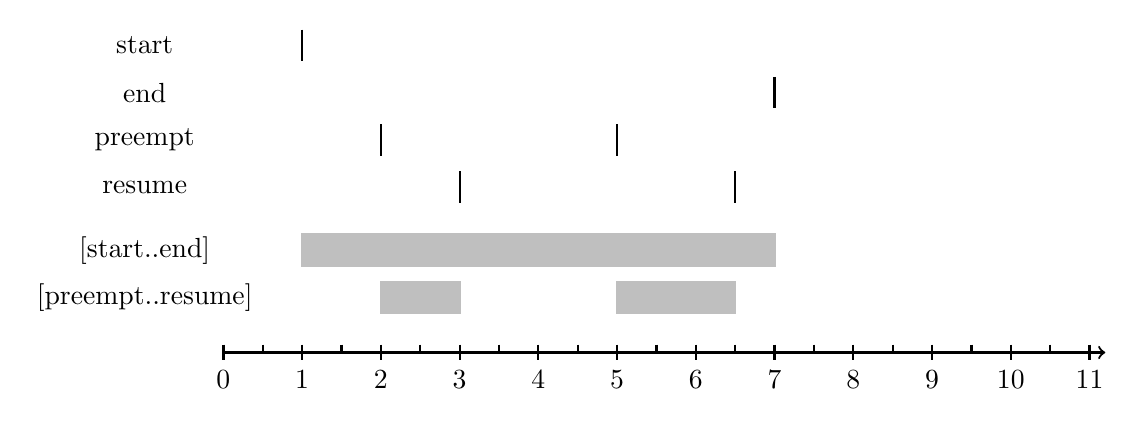
\begin{tikzpicture}[thick]
				% time axis
				\foreach \y in {-4}{
					\foreach \x in {0,...,11}
					\draw (\x,\y) -- (\x,\y-0.2) node[anchor=north] {\x};
					\foreach \x in {0.5,1.5,...,10.5}
					\draw (\x,\y) -- (\x,\y-0.1);
					\draw[->] (0,\y-0.1) -- (11.2, \y-0.1);
				}
				% start
				\node at (-1, -0.2) {start};
				\draw[] (1,0) -- (1,-0.4);
				% end
				\node at (-1, -0.8) {end};
				\draw[] (7, -0.6) -- (7, -1);
				%preempt
				\node at (-1, -1.4) {preempt};
				\draw[] (2, -1.2) -- (2, -1.6);
				\draw[] (5, -1.2) -- (5, -1.6);
				%resume
				\node at (-1, -2) {resume};
				\draw[] (3, -1.8) -- (3, -2.2);
				\draw[] (6.5, -1.8) -- (6.5, -2.2);
				
				\node at (-1, -2.8) {[start..end]};
				\draw [fill=lightgray, lightgray] (1, -2.6) rectangle (7, -3.0);
				
				\node at (-1, -3.4) {[preempt..resume]};
				\draw [fill=lightgray, lightgray] (2, -3.2) rectangle (3, -3.6);
				\draw [fill=lightgray, lightgray] (5, -3.2) rectangle (6.5, -3.6);
			\end{tikzpicture}
			\caption{Example ExecutionTimeConstraint}
			\label{fig:ExecutionTimeConstraintExample}
		\end{figure}
		
	\subsubsection{OrderConstraint}
		The \emph{OrderConstraint} takes two attributes
		\begin{align*}
			\emph{source} & \hspace{.5cm}\text{set of events}\\
			\emph{target} & \hspace{.5cm}\text{set of events}
		\end{align*}
		and is defined as\\[10pt]
		\begin{math}
			OrderConstraint ( source, target )\\
			\Leftrightarrow|source| = |target| \land \forall i:\exists x: x=source(i)\Rightarrow \exists y: y=target(i)\land < x \leq y
		\end{math}\\[10pt]
		This constraint ensures the order of events so that the $i^{th}$ event of $target$ occurs after the $i^{th}$ event of $source$. Also, the number of events in \emph{source} and \emph{target} must be equal.\\
		Figure~\ref{fig:OrderConstraintExample} visualizes an example of the \emph{OrderConstraint} with $source = \{1, 4, 6, 7\}$ and $target = \{3, 5, 9, 9.5\}$. The constraint is fulfilled because the number of elements is equal and each $i^{th}$ timestamp in \emph{target} is later than the $i^{th}$ timestamp of $source$.
		\begin{figure}
			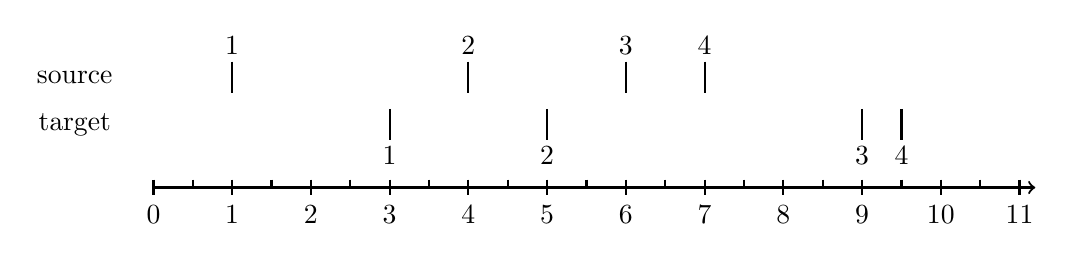
\begin{tikzpicture}[thick]
				% time axis
				\foreach \y in {-1.5}{
					\foreach \x in {0,...,11}
					\draw (\x,\y) -- (\x,\y-0.2) node[anchor=north] {\x};
					\foreach \x in {0.5,1.5,...,10.5}
					\draw (\x,\y) -- (\x,\y-0.1);
					\draw[->] (0,\y-0.1) -- (11.2, \y-0.1);
				}
				% start
				\node at (-1, -0.2) {source};
				\foreach \x in {1, 4, 6, 7}{
					\draw[] (\x,0) -- (\x,-0.4);
				}
				\node at (1, 0.2) {1};
				\node at (4, 0.2) {2};
				\node at (6, 0.2) {3};
				\node at (7, 0.2) {4};
				% end
				\node at (-1, -0.8) {target};
				\foreach \x in {3, 5, 9, 9.5}{
					\draw[] (\x,-0.6) -- (\x,-1);
				}
				\node at (3, -1.2) {1};
				\node at (5, -1.2) {2};
				\node at (9, -1.2) {3};
				\node at (9.5, -1.2) {4};
			\end{tikzpicture}
			\caption{Example OrderConstraint}
			\label{fig:OrderConstraintExample}
		\end{figure}
		
		
	\subsubsection{ComparisonConstraint}
		The \emph{ComparisonConstraint} is significantly different from all previous and following constraints, as it does not describe the behavior of events and only compares two time expressions. It takes three attributes
		\begin{align*}
			\emph{leftOperand} 	& \hspace{.5cm}\mathbb{T}\\
			\emph{rightOperand} & \hspace{.5cm}\mathbb{T}\\
			\emph{operator}		& \hspace{.5cm} \text{comparisonOperator}(\in \{LessThanOrEqual, LessThan,\\
								& \hspace{3.5cm} GreaterThanOrEqual, GreaterThan, Equal\})
		\end{align*}
		The definition is pretty straight forward as it only applies the given operator to the operands:\\[10pt]
		\begin{math}
			ComparisonConstraint(leftOperand, rightOperand, LessThanOrEqual)\\
				\Leftrightarrow leftOperand \leq rightOperand\\[5pt]
			ComparisonConstraint(leftOperand, rightOperand, LessThan)\\
				\Leftrightarrow leftOperand < rightOperand\\[5pt]
			ComparisonConstraint(leftOperand, rightOperand, GreaterThanOrEqual)\\
				\Leftrightarrow leftOperand \geq rightOperand\\[5pt]
			ComparisonConstraint(leftOperand, rightOperand, GreaterThan)\\
				\Leftrightarrow leftOperand > rightOperand\\[5pt]
			ComparisonConstraint(leftOperand, rightOperand, Equal)\\
				\Leftrightarrow leftOperand = rightOperand
		\end{math}\\[10pt]
		Due to the simplicity of this constraint, no explicit example is given.
		
	\subsubsection{SporadicConstraint}
		The \emph{SporadicConstraint} takes 5 attributes
		\begin{align*}
			\emph{event} 	& \hspace{.5cm}\text{set of events}\\
			\emph{lower} 	& \hspace{.5cm}\mathbb{T}\\
			\emph{upper} 	& \hspace{.5cm}\mathbb{T}\\
			\emph{jitter}	& \hspace{.5cm}\mathbb{T}\\
			\emph{minimum}	& \hspace{.5cm}\mathbb{T}
		\end{align*}
		and is defined as combination of the \emph{RepetitionConstraint} and the \emph{RepeatConstraint} as\\[10pt]
		\begin{math}
			SporadicConstraint ( event, lower, upper, jitter, minimum )\\
			\Leftrightarrow RepetitionConstraint(event, lower, upper, 1, jitter)\\
			\hspace*{.5cm}\land RepeatConstraint(event, minimum, \infty, 1)
		\end{math}\\[10pt]
		The second part of the definition, using the \emph{RepeatConstraint}, ensures that all events in \emph{event} lay at least \emph{minimum} apart. The application of the \emph{RepetitionConstraint} generates a set of events $X$ that lay between $lower$ and $upper$ apart from each other. For each point in time in $X$, there must be exactly one timestamp in \emph{event} that is not before the corresponding element of $X$ and not later than \emph{jitter} after that.\\
		Figure~\ref{fig:SporadicConstraintExample} shows a application of the \emph{SporadicConstraint} with the attributes $lower=2$, $upper=2.5$, $jitter=1$, $minimum=2$ and $event=\{1, 3.5, 6, 8.2, 10.5,...\}$. Like in the \emph{RepetitionConstraint}, the exact position of the timestamps in $X$ is variable and may need to be changed due to later entries in $event$.
		\begin{figure}
			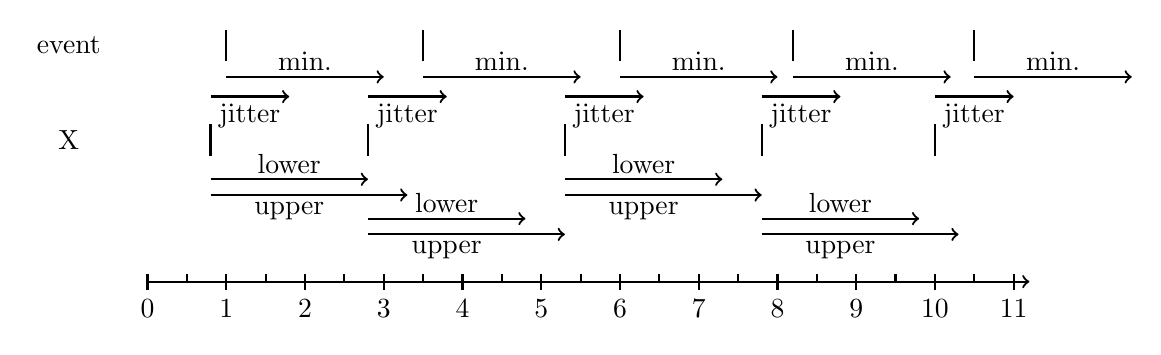
\begin{tikzpicture}[thick]
			% time axis
			\foreach \y in {-2.5}{
				\foreach \x in {0,...,11}
				\draw (\x,\y) -- (\x,\y-0.2) node[anchor=north] {\x};
				\foreach \x in {0.5,1.5,...,10.5}
				\draw (\x,\y) -- (\x,\y-0.1);
				\draw[->] (0,\y-0.1) -- (11.2, \y-0.1);
			}
			% event
			\node at (-1, 0.4) {event};
			\foreach \x in {1, 3.5, 6, 8.2, 10.5}{
				\draw[] (\x,0.2) -- (\x,+0.6);
				%minimum
				\draw[->] (\x, 0) -- (\x+2, 0);
				\node at (\x+1, 0.2) {min.};
			}
			% X
			\node at (-1, -0.8) {X};
			\foreach \x in {0.8, 2.8, 5.3, 7.8, 10}{
				\draw[] (\x,-0.6) -- (\x,-1);
				%jitter
				\draw[->] (\x, -0.25) -- (\x+1, -0.25);
				\node at (\x+0.5, -0.5) {jitter};
			}
			%lower/upper
			\foreach \x in {0.8, 5.3}{
				\node at (\x+1, -1.1){lower};
				\draw[->] (\x, -1.3) -- (\x+2, -1.3);
				\draw[->] (\x, -1.5) -- (\x+2.5, -1.5);
				\node at (\x+1, -1.7){upper};
			}
			\foreach \x in {2.8, 7.8}{
				\node at (\x+1, -1.6){lower};
				\draw[->] (\x, -1.8) -- (\x+2, -1.8);
				\draw[->] (\x, -2) -- (\x+2.5, -2);
				\node at (\x+1, -2.2){upper};
			}

			\end{tikzpicture}
			\caption{Example SporadicConstraint - $lower=2$, $upper=2.5$, $jitter=1$, $minimum=2$}
			\label{fig:SporadicConstraintExample}
		\end{figure}
	
	\subsubsection{PeriodicConstraint}
		The \emph{PeriodicConstraint} takes 4 attribute
		\begin{align*}
			\emph{event} 	& \hspace{.5cm}\text{set of events}\\
			\emph{period} 	& \hspace{.5cm}\mathbb{T}\\
			\emph{jitter}	& \hspace{.5cm}\mathbb{T}\\
			\emph{minimum}	& \hspace{.5cm}\mathbb{T}
		\end{align*}
		and defines a specialized form of the \emph{SporadicConstraint}\\[10pt]
		\begin{math}
			PeriodicConstraint ( event, period, jitter, minimum )\\
			\Leftrightarrow SporadicConstraint(event, period, period, jitter, minimum)
		\end{math}\\[10pt]
		The variable timestamps in the set $X$ are following a strictly periodic pattern, where subsequent elements of this set lay exactly \emph{period} apart. Each element of \emph{event} lays between one element of $X$ and \emph{jitter} after that. Again, there must be a bijective mapping between the elements of \emph{event} and $X$.\\
		In figure~\ref{fig:PeriodicConstraintExample}, the \emph{PeriodicConstraint} with the attributes $period=3$, $jitter=1$, $minimum=2.5$ and $event = \{1.2, 4.0, 8, 10.6, ...\}$ is visualized. The timestamps of $X$ lay exactly \emph{period} apart and the $events$ behind that in the previously described way. Also, the minimum time distance between all points of time in \emph{event} is \emph{minimum}.
		\begin{figure}
			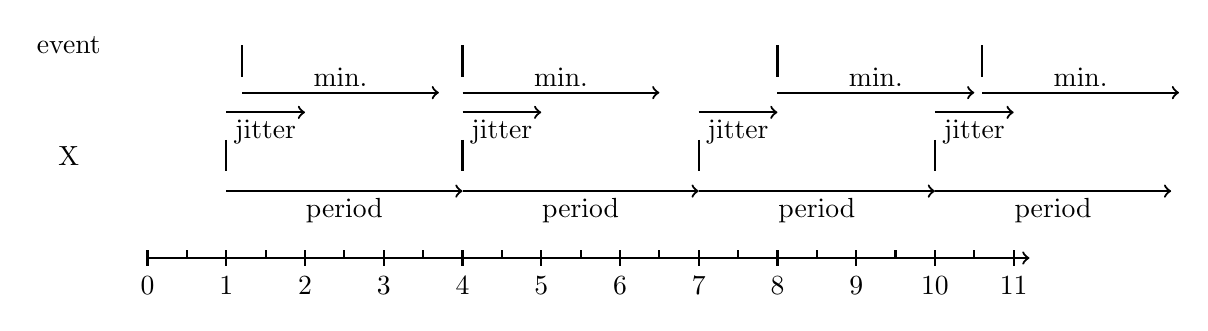
\begin{tikzpicture}[thick]
			% time axis
			\foreach \y in {-2}{
				\foreach \x in {0,...,11}
				\draw (\x,\y) -- (\x,\y-0.2) node[anchor=north] {\x};
				\foreach \x in {0.5,1.5,...,10.5}
				\draw (\x,\y) -- (\x,\y-0.1);
				\draw[->] (0,\y-0.1) -- (11.2, \y-0.1);
			}
			% event
			\node at (-1, 0.6) {event};
			\foreach \x in {1.2, 4.0, 8, 10.6}{
				%timestamp
				\draw[] (\x,0.2) -- (\x,+0.6);
				%minimum
				\draw[->] (\x, 0) -- (\x+2.5, 0);
				\node at (\x+1.25, 0.2) {min.};
			}
			% X
			\node at (-1, -0.8) {X};
			\foreach \x in {1, 4, 7, 10}{
				%timestamp
				\draw[] (\x,-0.6) -- (\x,-1);
				%jitter
				\draw[->] (\x, -0.25) -- (\x+1, -0.25);
				\node at (\x+0.5, -0.5) {jitter};
				%period
				\draw[->] (\x, -1.25) -- (\x+3, -1.25);
				\node at (\x+1.5, -1.5) {period};
			}
			\end{tikzpicture}
			\caption{Example PeriodicConstraint - $period=3$, $jitter=1$, $minimum=2.5$}
			\label{fig:PeriodicConstraintExample}
		\end{figure}
		
		
	\subsubsection{PatternConstraint}
		\label{sec:patterConstraintDefinition}
		The \emph{PatternConstraint} takes 5 attributes
		\begin{align*}
			\emph{event} 	& \hspace{.5cm}\text{set of events}\\
			\emph{period} 	& \hspace{.5cm}\mathbb{T}\\
			\emph{offset}	& \hspace{.5cm} \text{set of }\mathbb{T}\\
			\emph{jitter}	& \hspace{.5cm}\mathbb{T}\\
			\emph{minimum}	& \hspace{.5cm}\mathbb{T}
		\end{align*}
		and is defined as \\[10pt]
		\begin{math}
			PatternConstraint( event, period, \text{\textit{offset}}_1, ..., \text{\textit{offset}}_n, jitter, minimum )\\
			\Leftrightarrow\exists X: PeriodicConstraint(X, period, 0, 0)\\
			\text{\hspace{.5cm}} \land \forall i: DelayContraint(X, event, \text{\textit{offset}}_i,  \text{\textit{offset}}_i+jitter)\\
			\text{\hspace{.5cm}} \land RepeatConstraint(event, minimum, \infty, 1)
		\end{math}\\[10pt]
		This constraint can be understood as a modification of the \emph{PeriodicConstraint}, as it describes periodic behavior, but not from single events, but from groups of $| \text{\textit{offset}}_i|$ subsequent events, that follow specific time distances (specified by $\text{\textit{offset}}$) after the strictly periodic timestamps of $X$.\\
		There is a major weak spot in the definition of this constraint because the set $X$ can be set to the empty set. In this case, the part of the definition, which uses the \emph{PeriodicConstraint} and the \emph{DelayContraint}, is always satisfied, irrespective of the events in $event$. Therefore, the \emph{PatternConstraint} only ensures the minimal distance between two events, which should not be the purpose of this constraint. 
		The obvious countermeasure to this problem would be to restrict $X$ in a way that ensures that it is not empty and the first element of $X$ must lay before the first $event$ occurrence. The textual description of the constraint, which says literally the ''PatternConstraint requires the constrained event occurrences to appear at a predetermined series of offsets from a sequence of reference points'' contradicts this countermeasure because the \emph{DelayConstraint} allows additional events in the $target$ events with no matching $source$ event. Therefore, any event occurrences besides the events following the offset scheme would be allowed, which conflicts with the citation. Because of this problem, the \emph{PatternConstraint} is redefined as \\[10pt]
		\begin{math}
			PatternConstraint( event, period, \text{\textit{offset}}_1, ..., \text{\textit{offset}}_n, jitter, minimum )\\
			\Leftrightarrow\exists X: PeriodicConstraint(X, period, 0, 0)\\
			\text{\hspace{.5cm}} \land \forall i: \textbf{\emph{Strong}}DelayContraint(X, event, offset_i, offset_i+jitter)\\
			\text{\hspace{.5cm}} \land RepeatConstraint(event, minimum, \infty, 1)
		\end{math}\\[10pt]
		for the scope of this thesis. The usage of the \emph{StrongDelayConstraint}, instead of the \emph{DelayConstraint}, ensures that each event occurrence is following the time distances defined by the offsets. This notion of the \emph{PatternConstraint} is also carried by the described relations between the TADL2 timing constraints and the AUTOSAR Timing Extensions, which were done as part of the development of TADL2\cite{TIMMO2USE}. These descriptions equate the \emph{PatternConstraint} and AUTOSARs \emph{ConcretePatternEventTriggering}, which is clearly defined in the way of this redefinition.\\
		Figure~\ref{fig:PatternConstraintExample} shows an application of the \emph{PeriodicConstraint} with the attributes $period=5$, $\text{\textit{offset}}=\{1, 2, 2.5\}$, $jitter=0.5$, $minimum=0.5$ and\\
		$event = \{1.2, 2.2, 2.8, 6, 7, 8, 11.5, 12, 12.5, ...\}$. Like in the previously described constraint, the exact position of all points in time of $X$ may change due to later timestamps of $event$.
		\begin{figure}
			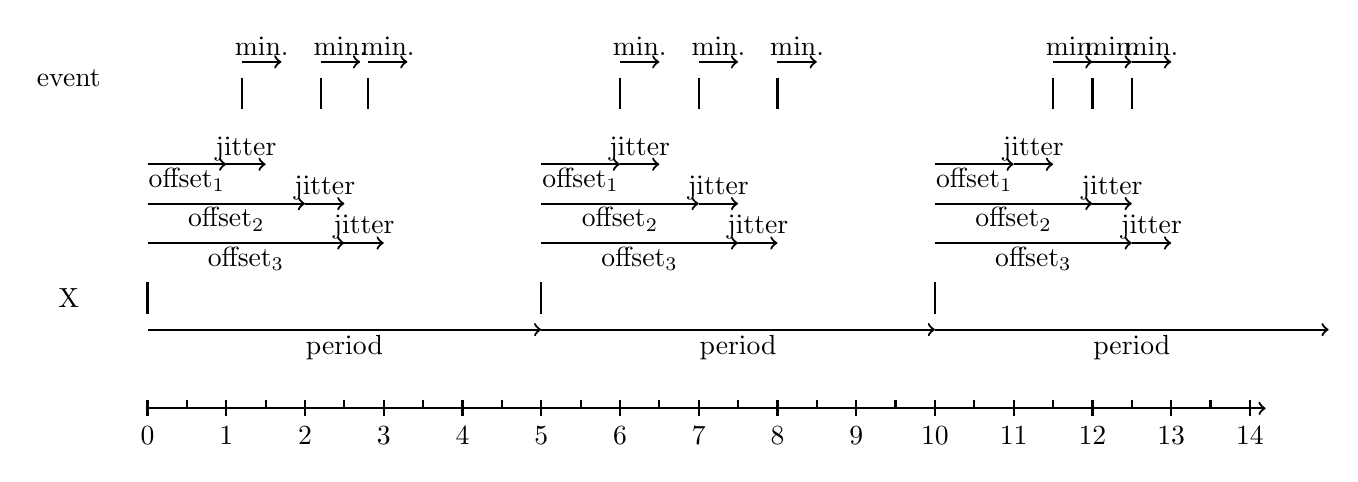
\begin{tikzpicture}[thick]
			% time axis
			\foreach \y in {-3.5}{
				\foreach \x in {0,...,14}
				\draw (\x,\y) -- (\x,\y-0.2) node[anchor=north] {\x};
				\foreach \x in {0.5,1.5,...,13.5}
				\draw (\x,\y) -- (\x,\y-0.1);
				\draw[->] (0,\y-0.1) -- (14.2, \y-0.1);
			}
			% event
			\node at (-1, 0.6) {event};
			\foreach \x in {1.2, 2.2, 2.8, 6, 7, 8, 11.5, 12, 12.5}{
				%timestamp
				\draw[] (\x,0.2) -- (\x,+0.6);
				%minimum
				\draw[->] (\x, 0.8) -- (\x+.5, 0.8);
				\node at (\x+0.25, 1) {min.};
			}
			% X
			\node at (-1, -2.2) {X};
			\foreach \x in {0,5, 10}{
				%timestamp
				\draw[] (\x,-2) -- (\x,-2.4);
				%offset 1
				\draw[->] (\x, -0.5) -- (\x+1, -0.5);
				\node at (\x+0.5, -0.7) {offset$_1$};
				\draw[->] (\x+1, -0.5) -- (\x+1.5, -0.5);
				\node at (\x+1.25, -0.3) {jitter};
				%offset 2
				\draw[->] (\x, -1) -- (\x+2, -1);
				\node at (\x+1, -1.2) {offset$_2$};
				\draw[->] (\x+2, -1) -- (\x+2.5, -1);
				\node at (\x+2.25, -0.8) {jitter};
				%offset 3
				\draw[->] (\x, -1.5) -- (\x+2.5, -1.5);
				\node at (\x+1.25, -1.7) {offset$_3$};
				\draw[->] (\x+2.5, -1.5) -- (\x+3, -1.5);
				\node at (\x+2.75, -1.3) {jitter};
				%period
				\draw[->] (\x, -2.6) -- (\x+5, -2.6);
				\node at (\x+2.5, -2.83) {period};
			}
			\end{tikzpicture}
			\caption{Example PatternConstraint - $period=5$, $offset=\{1, 2, 2.5\}$, $jitter=0.5$, $minimum=0.5$}
			\label{fig:PatternConstraintExample}
		\end{figure}
		
	\subsubsection{ArbitraryConstraint}
		The \emph{ArbitraryConstraint} takes 3 attributes
		\begin{align*}
			\emph{event} 	& \hspace{.5cm}\text{set of events}\\
			\emph{minimum}	& \hspace{.5cm}\text{set of }\mathbb{T}\\
			\emph{maximum}	& \hspace{.5cm}\text{set of }\mathbb{T}
		\end{align*}
		where $|minimum|=|maximum|$. It is defined as \\[10pt]
		\begin{math}\\
			ArbitraryConstraint ( event, minimum_1, ..., minimum_n, maximum_1, ..., maximum_n)\\
			\Leftrightarrow\forall i: RepeatConstraint(event, minimum_i, maximum_i, i)
		\end{math}\\[10pt]
		The idea behind the \emph{ArbitraryConstraint} is to describe the time distance between each event and several following events. The first entry of \emph{minimum} and \emph{maximum} defines the distance between every event and its direct successor. The second entry, where the \emph{span} attribute of the  \emph{RepeatConstraint} is 2, defines the distance between one event and its next but one successor and so on.\\
		Figure~\ref{fig:ArbitraryConstraintExample} shows an example of the \emph{ArbitraryConstraint} with the attributes $minimum=\{1,2,3\}$, $maximum=\{5,6,7\}$ and $event=\{1, 2, 3, 5, 8, 10, ...\}$. The time distances between subsequent events with 0, 1, 2 and more skipped events are shown in table~\ref{tab:ArbitraryConstraintExampleTable}. The relevant distances are written in \textbf{bold} font. The time distances are matching the ranges given by the $minimum$- and $maximum$ attributes.\\
		\begin{table}
			\begin{tabular}{|c|c|c|c|c|c|c|}
				\hline
				& 1 & 2 & 3 & 5 & 8 & 10 \\
				\hline
				1 & 0 & \textbf{1} & \textbf{2} & \textbf{4} & 7 & 9 \\
				\hline
				2 &  & 0 & \textbf{1} & \textbf{3} & \textbf{6} & 8 \\
				\hline
				3 &  &  & 0 & \textbf{2} & \textbf{5} & \textbf{7} \\
				\hline
				5 &  &  &  & 0 & \textbf{3} & \textbf{5} \\
				\hline
				8 &  &  &  &  & 0 & \textbf{2} \\
				\hline
				10 &  &  &  &  &  & 0 \\
				\hline
			\end{tabular}
			\centering
			\caption{Time distances as seen in figure~\ref{fig:ArbitraryConstraintExample}}
			\label{tab:ArbitraryConstraintExampleTable}
		\end{table}

		\begin{figure}
			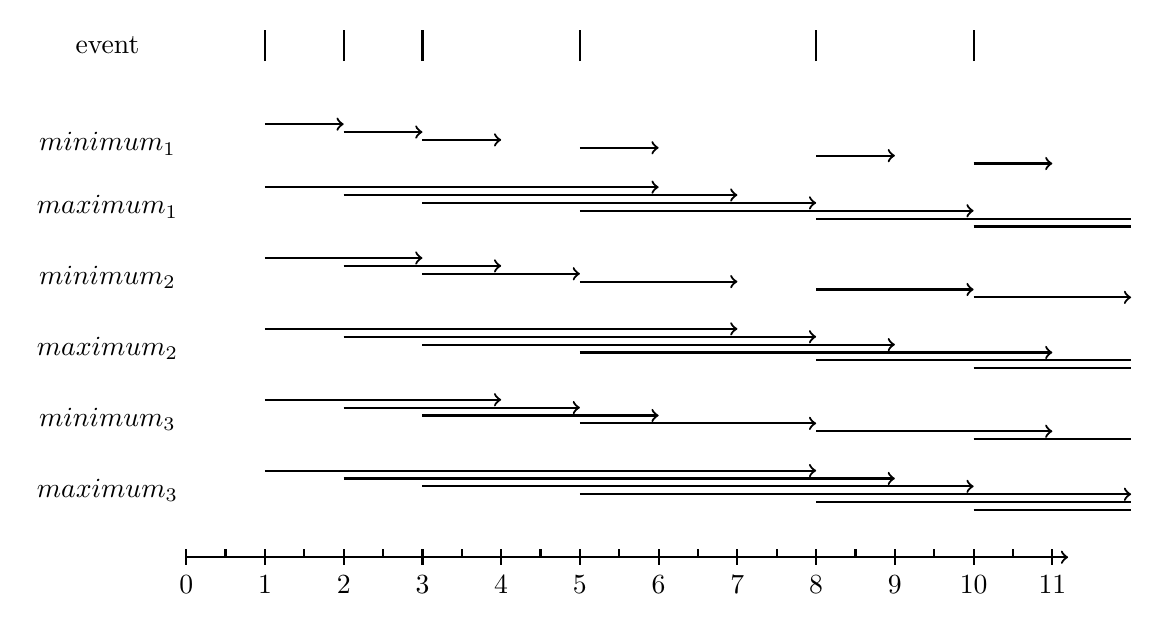
\begin{tikzpicture}[thick]
			% time axis
			\foreach \y in {-6}{
				\foreach \x in {0,...,11}
				\draw (\x,\y) -- (\x,\y-0.2) node[anchor=north] {\x};
				\foreach \x in {0.5,1.5,...,10.5}
				\draw (\x,\y) -- (\x,\y-0.1);
				\draw[->] (0,\y-0.1) -- (11.2, \y-0.1);
			}
			% event
			\node at (-1, 0.4) {event};
			\node at (-1, -0.85) {$minimum_1$};
			\node at (-1, -1.65) {$maximum_1$};
			
			\node at (-1, -2.55) {$minimum_2$};
			\node at (-1, -3.45) {$maximum_2$};
			
			
			\node at (-1, -4.35) {$minimum_3$};
			\node at (-1, -5.25) {$maximum_3$};
			\foreach \x in {1,2,3,5,8,10}{
				%timestamp
				\draw[] (\x,0.2) -- (\x,+0.6);
			}
			% minimum 1
			\draw[->] (1, -0.6) -- (2, -0.6);
			\draw[->] (2, -0.7) -- (3, -0.7);
			\draw[->] (3, -0.8) -- (4, -0.8);
			\draw[->] (5, -0.9) -- (6, -0.9);
			\draw[->] (8, -1.0) -- (9, -1.0);
			\draw[->] (10, -1.1) -- (11, -1.1);
			% maximum 1
			\draw[->] (1, -1.4) -- (6, -1.4);
			\draw[->] (2, -1.5) -- (7, -1.5);
			\draw[->] (3, -1.6) -- (8, -1.6);
			\draw[->] (5, -1.7) -- (10, -1.7);
			\draw[-] (8, -1.8) -- (12, -1.8);
			\draw[-] (10, -1.9) -- (12, -1.9);
			
			% minimum 2
			\draw[->] (1, -2.3) -- (3, -2.3);
			\draw[->] (2, -2.4) -- (4, -2.4);
			\draw[->] (3, -2.5) -- (5, -2.5);
			\draw[->] (5, -2.6) -- (7, -2.6);
			\draw[->] (8, -2.7) -- (10, -2.7);
			\draw[->] (10, -2.8) -- (12, -2.8);
			
			% maximum 2
			\draw[->] (1, -3.2) -- (7, -3.2);
			\draw[->] (2, -3.3) -- (8, -3.3);
			\draw[->] (3, -3.4) -- (9, -3.4);
			\draw[->] (5, -3.5) -- (11, -3.5);
			\draw[-] (8, -3.6) -- (12, -3.6);
			\draw[-] (10, -3.7) -- (12, -3.7);
			
			% minimum 3
			\draw[->] (1, -4.1) -- (4, -4.1);
			\draw[->] (2, -4.2) -- (5, -4.2);
			\draw[->] (3, -4.3) -- (6, -4.3);
			\draw[->] (5, -4.4) -- (8, -4.4);
			\draw[->] (8, -4.5) -- (11, -4.5);
			\draw[-] (10, -4.6) -- (12, -4.6);
			
			% maximum 3
			\draw[->] (1, -5.0) -- (8, -5.0);
			\draw[->] (2, -5.1) -- (9, -5.1);
			\draw[->] (3, -5.2) -- (10, -5.2);
			\draw[->] (5, -5.3) -- (12, -5.3);
			\draw[-] (8, -5.4) -- (12, -5.4);
			\draw[-] (10, -5.5) -- (12, -5.5);
			
			
			\end{tikzpicture}
			\caption{Example ArbitraryConstraint - $minimum=\{1,2,3\}$ and $minimum=\{4,5,6\}$}
			\label{fig:ArbitraryConstraintExample}
		\end{figure}
		
	\subsubsection{BurstConstraint}
		The \emph{BurstConstraint} takes 4 attributes
		\begin{align*}
			\emph{event} 			& \hspace{.5cm}\text{set of events}\\
			\emph{length}			& \hspace{.5cm} \mathbb{T}\\
			\emph{maxOccurrences}	& \hspace{.5cm} integer\\
			\emph{minimum}			& \hspace{.5cm} \mathbb{T}
		\end{align*}
		and is defined as \\[10pt]
		\begin{math}
			BurstConstraint ( event, length, maxOccurrences, minimum )\\
			\Leftrightarrow RepeatConstraint(event, length, \infty, maxOccurrences)\\
			\text{\hspace{.5cm}}\land RepeatConstraint(event, minimum, \infty, 1)
		\end{math}\\[10pt]
		 This constraint defines the maximum number of events in a time interval of the given $length$. Additionally, all subsequent events must be at least \emph{minimum} apart. Therefore, the intuition is different from the AUTOSAR \emph{BurstPatternEventTriggering}, where clusters of events are described. A complete comparison of these constraints will be made in section~\ref{comparisonConstraints}.\\
		 In figure~\ref{fig:BurstConstraintExample}, an application of the \emph{BurstConstraint} with the attributes $length=5$, $maxOccurrences=3$, $minimum=0.8$ and $event = \{1,2,3,7,8,9\}$ is visualized. In every interval of length 5, there are three or fewer events. Also, all subsequent events lay at least $0.8$ apart. Therefore, the constraint is fulfilled.
 		\begin{figure}
		 	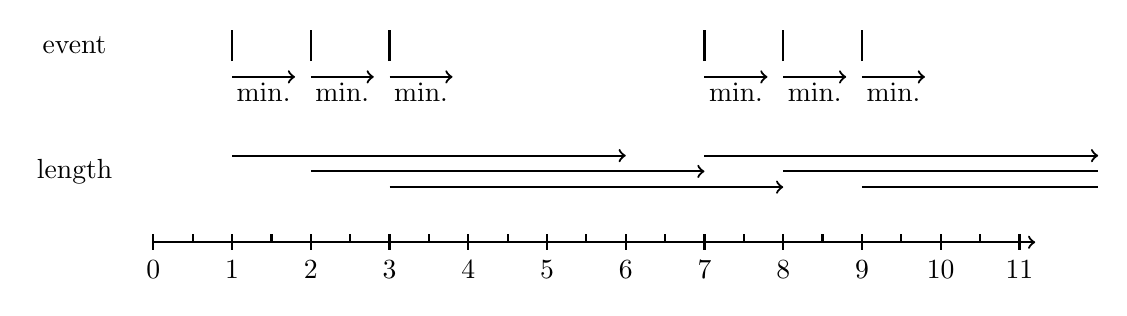
\begin{tikzpicture}[thick]
			 	% time axis
			 	\foreach \y in {-2}{
			 		\foreach \x in {0,...,11}
			 		\draw (\x,\y) -- (\x,\y-0.2) node[anchor=north] {\x};
			 		\foreach \x in {0.5,1.5,...,10.5}
			 		\draw (\x,\y) -- (\x,\y-0.1);
			 		\draw[->] (0,\y-0.1) -- (11.2, \y-0.1);
			 	}
			 	% event
			 	\node at (-1, 0.4) {event};
			 	\foreach \x in {1, 2, 3, 7, 8, 9}{
			 		%timestamp
			 		\draw[] (\x,0.2) -- (\x,+0.6);
			 		%minimum
			 		\draw[->] (\x, 0) -- (\x+0.8, 0);
			 		\node at (\x+0.4, -0.2) {min.};
			 	}
		 		% length
		 		\node at (-1, -1.2) {length};
		 		\draw[->] (1, -1) -- (6, -1);
	 			\draw[->] (2, -1.2) -- (7, -1.2);
 				\draw[->] (3, -1.4) -- (8, -1.4);
 				\draw[->] (7, -1) -- (12, -1);
 				\draw[-] (8, -1.2) -- (12, -1.2);
 				\draw[-] (9, -1.4) -- (12, -1.4);
		 	\end{tikzpicture}
		 	\caption{Example BurstConstraint - $length=5$, $maxOccurences=3$ $minimum=0.8$}
		 	\label{fig:BurstConstraintExample}
		 \end{figure}
	
	\subsubsection{ReactionConstraint}
		The \emph{ReactionConstraint} takes 3 attributes
		\begin{align*}
			\emph{scope} 	& \hspace{.5cm} EventChain\\
			\emph{minimum}	& \hspace{.5cm} \mathbb{T}\\
			\emph{maximum}	& \hspace{.5cm} \mathbb{T}
		\end{align*}
		and is defined as \\[10pt]
		\begin{math}
			ReactionConstraint ( scope, minimum, maximum )\\
			\Leftrightarrow\forall x\in scope.stimulus: \exists y\in scope.response:\\
			\text{\hspace{.5cm}}x.color=y.color\\
			\text{\hspace{.5cm}}\land (\forall y'\in scope.response: y'.color=y.color\Rightarrow y\leq y')\\
			\text{\hspace{.5cm}}\land minimum \leq y-x \leq maximum
		\end{math}\\[10pt]
		The definition says that after every event $x$ of $scope.stimulus$, there is an event $y$ in $scope.response$ with the same color. The time distance between these events must be at least $minimum$ and at most $maximum$. Additional events with the same color as $y$ in $scope.response$ are allowed if they lay behind $y$.  The definition implies that additional events with other colors are allowed in $scope.response$, but not in $scope.stimulus$.\\
		A visualized example with the attributes $minimum=1$, $maximum=3$,\\
		$scope.stimulus=\{(1, red), (5, green), (5.5, purple), (8, orange)\}$ and $scope.response=\{(0.8, blue), (2.1, red), (4.5, blue), (6.6, purple),
		(6.7, purple), (9.5, purple), (7.5, green), \\
		(10, orange)\}$ can be seen in figure~\ref{fig:ReactionConstraint}. The red $stimulus$ event is followed by the red $response$-event at 2.1, the green $stimulus$ event at 5 by the $response$ event at 7.5 and so on. The blue $response$ events at 1 and 4.5 are additional events without an associated stimulus event. The purple events at 6.7 and 9.5 are the second and third events of this color in $scope.response$ Therefore, their time distance to the $stimulus$ event with the same color is irrelevant.
 		\begin{figure}
			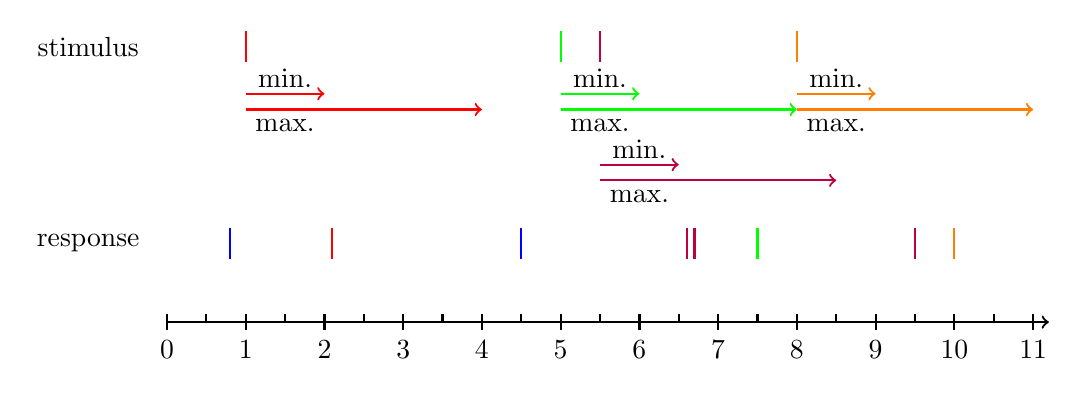
\begin{tikzpicture}[thick]
				% time axis
				\foreach \y in {-3}{
					\foreach \x in {0,...,11}
					\draw (\x,\y) -- (\x,\y-0.2) node[anchor=north] {\x};
					\foreach \x in {0.5,1.5,...,10.5}
					\draw (\x,\y) -- (\x,\y-0.1);
					\draw[->] (0,\y-0.1) -- (11.2, \y-0.1);
				}
				% stimulus
				\node at (-1, 0.4) {stimulus};
				\draw[red, thick]    (1  ,0.2) -- (1,+0.6);
				\draw[green, thick]  (5  ,0.2) -- (5,+0.6);
				\draw[purple, thick] (5.5,0.2) -- (5.5,+0.6);
				\draw[orange, thick] (8  ,0.2) -- (8,+0.6);
				
				% minimum
				\draw[->, red] (1, -0.2) -- (2, -0.2);
				\node at (1.5, 0) {min.};
				\draw[->, green] (5, -0.2) -- (6, -0.2);
				\node at (5.5, 0) {min.};
				\draw[->, purple] (5.5, -1.1) -- (6.5, -1.1);
				\node at (6, -0.9) {min.};
				\draw[->, orange] (8, -0.2) -- (9, -0.2);
				\node at (8.5, 0) {min.};
				%maximum
				\draw[->, red] (1, -0.4) -- (4, -0.4);
				\node at (1.5, -0.6) {max.};
				\draw[->, green] (5, -0.4) -- (8, -0.4);
				\node at (5.5, -0.6) {max.};
				\draw[->, purple] (5.5, -1.3) -- (8.5, -1.3);
				\node at (6, -1.5) {max.};
				\draw[->, orange] (8, -0.4) -- (11, -0.4);
				\node at (8.5, -0.6) {max.};
				%response
				\node at (-1, -2.1) {response};
				\draw[blue, thick]    (.8  ,-1.9) -- (.8,-2.3);
				\draw[blue, thick]    (4.5  ,-1.9) -- (4.5,-2.3);
				\draw[red, thick]    (2.1  ,-1.9) -- (2.1,-2.3);
				\draw[green, thick]  (7.5  ,-1.9) -- (7.5,-2.3);
				\draw[purple, thick] (6.6,-1.9) -- (6.6,-2.3);
				\draw[purple, thick] (6.7,-1.9) -- (6.7,-2.3);
				\draw[purple, thick] (9.5,-1.9) -- (9.5,-2.3);
				\draw[orange, thick] (10  ,-1.9) -- (10,-2.3);
			\end{tikzpicture}
			\caption{Example ReactionConstraint - $minimum=1$, $maximum=3$}
			\label{fig:ReactionConstraint}
		\end{figure}
		
	
	\subsubsection{AgeConstraint}
		The \emph{AgeConstraint} takes 3 attributes
		\begin{align*}
			\emph{scope} 	& \hspace{.5cm} EventChain\\
			\emph{minimum}	& \hspace{.5cm} \mathbb{T}\\
			\emph{maximum}	& \hspace{.5cm} \mathbb{T}
		\end{align*}
		and is defined as \\[10pt]
		\begin{math}
			AgeConstraint ( scope, minimum, maximum )\\
			\Leftrightarrow\forall y\in scope.response: \exists x\in scope.stimulus:\\
			\text{\hspace{.5cm}}x.color=y.color\\
			\text{\hspace{.5cm}}\land (\forall x'\in scope.stimulus: x'.color=x.color\Rightarrow x'\leq x)\\
			\text{\hspace{.5cm}}\land minimum \leq y-x \leq maximum
		\end{math}\\[10pt]
		The \emph{AgeConstraint} is a turned around counterpart to the \emph{ReactionConstraint}. For every event of $scope.response$, there must be an event with the same color in $scope.stimulus$. The time distance between these events must be between $minimum$ and $maximum$. Additional events are only allowed in $scope.stimulus$ and only before the event that matches with a $response$ event, which is implied by the correctness of the event chain.\\
		Figure~ \ref{fig:AgeConstraint} shows an application of the \emph{AgeConstraint} with the attributes $minimum=1$, $maximum=3$, $scope.stimulus=\{(0.8, blue), (1, red), (2, green), (4.5, green),\\
		(5, green), (5.5, purple), (8, orange)\}$ and $scope.response=\{(3.5, red), (7.5, green),\\
		 (6.6, purple), (10, orange)\}$. The blue timestamps are additional events without matching events in $scope.response$.
 		\begin{figure}
			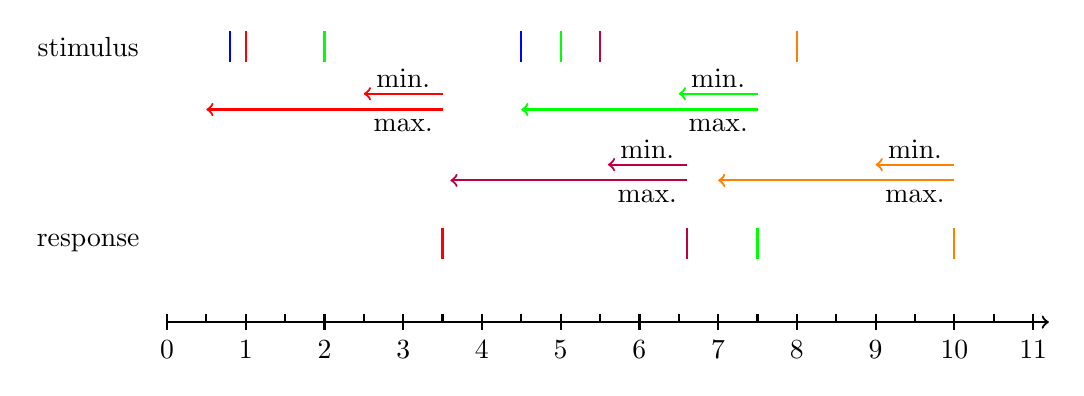
\begin{tikzpicture}[thick]
				% time axis
				\foreach \y in {-3}{
					\foreach \x in {0,...,11}
					\draw (\x,\y) -- (\x,\y-0.2) node[anchor=north] {\x};
					\foreach \x in {0.5,1.5,...,10.5}
					\draw (\x,\y) -- (\x,\y-0.1);
					\draw[->] (0,\y-0.1) -- (11.2, \y-0.1);
				}
				% stimulus
				\node at (-1, 0.4) {stimulus};
				\draw[red, thick]    (1  ,0.2) -- (1,+0.6);
				\draw[green, thick]  (2  ,0.2) -- (2,+0.6);
				\draw[green, thick]  (5  ,0.2) -- (5,+0.6);
				\draw[purple, thick] (5.5,0.2) -- (5.5,+0.6);
				\draw[orange, thick] (8  ,0.2) -- (8,+0.6);
				\draw[blue, thick] (0.8, 0.2) -- (0.8,0.6);
				\draw[blue, thick] (4.5, 0.2) -- (4.5,0.6);
				
				% minimum
				\draw[->, red] (3.5, -0.2) -- (2.5, -0.2);
				\node at (3, 0) {min.};
				\draw[->, green] (7.5, -0.2) -- (6.5, -0.2);
				\node at (7, 0) {min.};
				\draw[->, purple] (6.6, -1.1) -- (5.6, -1.1);
				\node at (6.1, -0.9) {min.};
				\draw[->, orange] (10, -1.1) -- (9, -1.1);
				\node at (9.5, -0.9) {min.};
				%maximum
				\draw[->, red] (3.5, -0.4) -- (0.5, -0.4);
				\node at (3, -0.6) {max.};
				\draw[->, green] (7.5, -0.4) -- (4.5, -0.4);
				\node at (7, -0.6) {max.};
				\draw[->, purple] (6.6, -1.3) -- (3.6, -1.3);
				\node at (6.1, -1.5) {max.};
				\draw[->, orange] (10, -1.3) -- (7, -1.3);
				\node at (9.5, -1.5) {max.};
				%response
				\node at (-1, -2.1) {response};
				\draw[red, thick]    (3.5  ,-1.9) -- (3.5,-2.3);
				\draw[green, thick]  (7.5  ,-1.9) -- (7.5,-2.3);
				\draw[purple, thick] (6.6,-1.9) -- (6.6,-2.3);
				%\draw[purple, thick] (6.7,-1.9) -- (6.7,-2.3);
				%\draw[purple, thick] (9.5,-1.9) -- (9.5,-2.3);
				\draw[orange, thick] (10  ,-1.9) -- (10,-2.3);
			\end{tikzpicture}
			\caption{Example AgeConstraint - $minimum=1$, $maximum=3$}
			\label{fig:AgeConstraint}
		\end{figure}
		
	\subsubsection{OutputSynchronizationConstraint}
		The \emph{OutputSynchronizationConstraint} takes 2 attributes
		\begin{align*}
			\emph{scope} 	& \hspace{.5cm} \text{Set of }EventChain\\
			\emph{tolerance}	& \hspace{.5cm} \mathbb{T}
		\end{align*}
		where all elements of \emph{scope} have the same $stimulus$ event set. It is defined as \\[10pt]
		\begin{math}
			OutputSynchronizationConstraint ( scope_1, ..., scope_n, tolerance )\\
			\Leftrightarrow\forall x\in scope_1.stimulus: \exists t: \forall i: \exists y\in scope_i.response:\\
			\text{\hspace{.5cm}} x.color = y.color\\
			\text{\hspace{.5cm}}\land (\forall y'\in scope_i.response: y'.color=y.color \Rightarrow y\leq y')\\
			\text{\hspace{.5cm}}\land 0\leq y-t\leq tolerance
		\end{math}\\[10pt]
		The definition says that after each event $x$ in $scope_1.stimulus$, there must be an interval with the length of $tolerance$, in which every $scope_i.response$ must have an event $y$ with the same color as $x$. Additional response events with this color are only allowed after $y$.
		Figure~\ref{fig:OutputSynchronizationConstraint} shows an example of the \emph{OutputSynchronizationConstraint} with the attributes $tolerance = 1$,\\
		 $scope[1].stimulus=scope[2].stimulus=scope[3].stimulus=\{(1, red), (4, green), (5, purple)\}$,\\
		$scope[1].response=\{(2, red), (6, purple), (6.2, purple), (8.2, green)\}$,\\
		$scope[2].response=\{(2.6, red), (6.2, purple), (8, green), (10.5, green)\}$,\\
		$scope[3].response=\{(2.3, red), (6.5, purple), (8.5, green)\}$.\\
		
 		\begin{figure}
			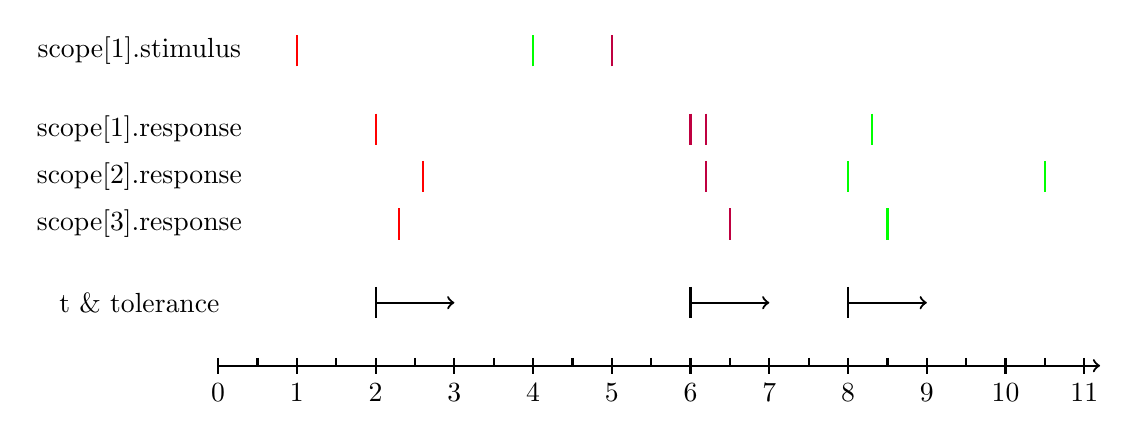
\begin{tikzpicture}[thick]
				% time axis
				\foreach \y in {-3.5}{
					\foreach \x in {0,...,11}
					\draw (\x,\y) -- (\x,\y-0.2) node[anchor=north] {\x};
					\foreach \x in {0.5,1.5,...,10.5}
					\draw (\x,\y) -- (\x,\y-0.1);
					\draw[->] (0,\y-0.1) -- (11.2, \y-0.1);
				}
				% stimulus
				\node at (-1, 0.4) {scope\textcolor{black}{[1]}.stimulus};
				\draw[red, thick]    (1  ,0.2) -- (1,+0.6);
				\draw[green, thick]  (4  ,0.2) -- (4,+0.6);
				\draw[purple, thick] (5,0.2) -- (5,+0.6);
				
				\node at(-1, -0.6) {scope[1].response};
				\draw[red, thick]    (2, -0.4) -- (2, -0.8);
				\draw[green, thick]  (8.3, -0.4) -- (8.3, -0.8);
				\draw[purple, thick] (6, -0.4) -- (6, -0.8);
				\draw[purple, thick] (6.2, -0.4) -- (6.2, -0.8);
				
				\node at(-1, -1.2) {scope[2].response};
				\draw[red, thick]    (2.6, -1) -- (2.6, -1.4);
				\draw[green, thick]    (8, -1) -- (8, -1.4);
				\draw[green, thick]    (10.5, -1) -- (10.5, -1.4);
				\draw[purple, thick]    (6.2, -1) -- (6.2, -1.4);
				
				\node at(-1, -1.8) {scope[3].response};
				\draw[red, thick]    (2.3, -1.6) -- (2.3, -2);
				\draw[green, thick]  (8.5, -1.6) -- (8.5, -2);
				\draw[purple, thick] (6.5, -1.6) -- (6.5, -2);
				
				\node at (-1, -2.8) {t \& tolerance};
				\foreach \i in {2, 6, 8} {
					\draw[thick] (\i, -2.6) -- (\i, -3);
					\draw[->] (\i, -2.8) -- (\i+1, -2.8);
				}

			\end{tikzpicture}
			\caption{Example OutputSynchronizationConstraint - $tolerance=1$}
			\label{fig:OutputSynchronizationConstraint}
		\end{figure}
		
	\subsubsection{InputSynchronizationConstraint}
	The \emph{InputSynchronizationConstraint} takes 2 attributes
	\begin{align*}
		\emph{scope} 	& \hspace{.5cm} \text{Set of }EventChain\\
		\emph{tolerance}& \hspace{.5cm} \mathbb{T}
	\end{align*}
	where all elements of \emph{scope} have the same $response$ event set. It is defined as \\[10pt]
	\begin{math}\\
		InputSynchronizationConstraint ( scope_1, ..., scope_n, tolerance )\\
		\Leftrightarrow\forall y\in scope_1.response: \exists t: \forall i: \exists x\in scope_i.stimulus:\\
		\text{\hspace{.5cm}} x.color = y.color\\
		\text{\hspace{.5cm}}\land (\forall x'\in scope_i.stimulus: x'.color=x.color \Rightarrow x\leq x')\\
		\text{\hspace{.5cm}}\land 0\leq x-t\leq tolerance
	\end{math}\\[10pt]
	The \emph{InputSynchronizationConstraint} is a counterpart of the \emph{OutputSynchronizationConstraint}, as the \emph{stimulus} events must be synchronized, not the \emph{response} events.\\
	Figure~\ref{fig:InputSynchronizationConstraint} contains an example of the \emph{InputSynchronizationConstraint} with the attributes $tolerance=1$\\
	$scope[1].stimulus=\{(1, red), (1.5, green), (4.6, green), (8, purple)\}$\\
	$scope[2].stimulus=\{(1.2, red), (4, green), (8.3, purple), (8.5, purple)\}$\\
	$scope[3].stimulus=\{(1.5, red), (4, green), (8.9, purple)\}$\\
	$scope[1].response=scope[2].response=scope[3].response=\{(2.5, red), (6, green), (10, purple)\}$\\
	\begin{figure}
		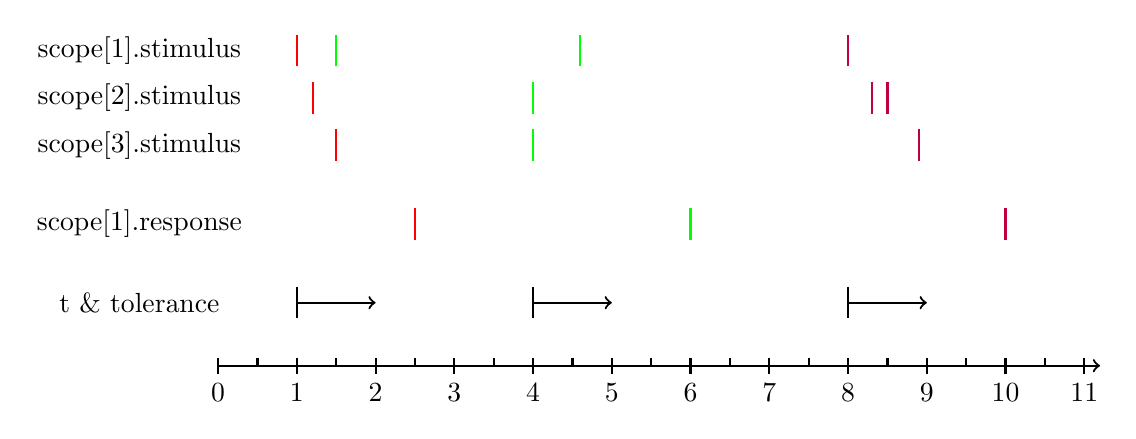
\begin{tikzpicture}[thick]
			% time axis
			\foreach \y in {-3.5}{
				\foreach \x in {0,...,11}
				\draw (\x,\y) -- (\x,\y-0.2) node[anchor=north] {\x};
				\foreach \x in {0.5,1.5,...,10.5}
				\draw (\x,\y) -- (\x,\y-0.1);
				\draw[->] (0,\y-0.1) -- (11.2, \y-0.1);
			}
			% stimulus
			\node at (-1, 0.4) {scope[1].stimulus};
			\draw[red, thick]    (1  ,0.2) -- (1,+0.6);
			\draw[green, thick]  (1.5  ,0.2) -- (1.5,+0.6);
			\draw[green, thick]  (4.6  ,0.2) -- (4.6,+0.6);
			\draw[purple, thick] (8,0.2) -- (8,+0.6);
			
			\node at (-1, -0.2) {scope[2].stimulus};
			\draw[red, thick]    (1.2,0) -- (1.2, -0.4);
			\draw[green, thick]  (4  ,0) -- (4,-0.4);
			\draw[purple, thick] (8.3,  0) -- (8.3,-0.4);
			\draw[purple, thick] (8.5,  0) -- (8.5,-0.4);
			
			\node at (-1, -0.8) {scope[3].stimulus};
			\draw[red, thick]    (1.5,-0.6) -- (1.5, -1);
			\draw[green, thick]  (4,  -0.6) -- (4,-1);
			\draw[purple, thick] (8.9,-0.6) -- (8.9,-1);
			
			\node at(-1, -1.8) {scope[1].response};
			\draw[red, thick]    (2.5, -1.6) -- (2.5, -2);
			\draw[green, thick]  (6, -1.6) -- (6, -2);
			\draw[purple, thick] (10, -1.6) -- (10, -2);
			
			\node at (-1, -2.8) {t \& tolerance};
			\foreach \i in {1, 4, 8} {
				\draw[thick] (\i, -2.6) -- (\i, -3);
				\draw[->] (\i, -2.8) -- (\i+1, -2.8);
			}
			
		\end{tikzpicture}
		\caption{Example InputSynchronizationConstraint - $tolerance=1$}
		\label{fig:InputSynchronizationConstraint}
	\end{figure}
			
\subsection{Comparison TADL2 - AUTOSAR Timing Extension}
\label{comparisonConstraints}
	As said before, the \emph{TADL2 Timing Constraints} and the \emph{AUTOSAR Timing Extensions} are compatible in parts. Many of the \emph{AUTOSAR Timing Extension} can be expressed as equivalent combinations of the \emph{TADL2 Timing Constraints}. In \cite{TIMMO2USE}, the relationship between these constraints is shown, but this comparison is based on an outdated AUTOSAR version. Therefore each \textit{AUTOSAR Timing Extensions} will be listed in this chapter, and it will be explained if and how they can be expressed using \textit{TADL2 Timing Constraints}.\\
	The types used in the AUTOSAR Timing Extension are similar to the ones in TADL2. TADL2 \emph{Events} are called \emph{TimingDescriptionEvent} in AUTOSAR. The same goes for \emph{EventChains}, which are called \emph{TimingDescriptionEventChains}. A larger difference can be seen in the definition of time. While TADL2 defines time as real numbers, the time definition used in the AUTOSAR Timing Extension can also be multidimensional, for example, when the real time and the crankshaft angle are regarded. For simplification, all timestamps are considered as real numbers in the following, but an extension to multidimensional time stamps is possible, as AUTOSAR requires a strict order between all time stamps. Some of the AUTOSAR Timing Extensions are defined on \emph{Executable Entities}, which describe things, that can be executed. An example of this is a program routine, which starts and finishes at certain times. In the analysis of their timing, only striking points in time of these entities are relevant, like the start and endpoints or interruptions. Therefore \emph{Executable Entities} can be transformed into events if needed.
	
	It should be noted that the set of TADL2 timing constraints are not equal to the AUTOSAR Timing Extension and that there are constraints that cannot be expressed using the corresponding counterpart.

	\subsubsection{PeriodicEventTriggering}
		The \emph{PeriodicEventTriggering} defined in AUTOSAR with the attributes\\ $(\textcolor{black}{event}, period, jitter, minimumInterArrivalTime)$ is equivalent to the \emph{TADL2} \emph{PeriodicConstraint} with the same attributes.
		
	\subsubsection{SporadicEventTriggering}
		AUTOSARs \emph{SporadicEventTriggering} with the attributes\\
		 $(\textcolor{black}{event}, jitter, maximumInterArrivalTime,  minimumInterArrivalTime, period)$ is equivalent to the \emph{TADL2} \emph{SporadicConstraint}, except for the names of the attributes:\\
		\begin{math}
			lower\widehat{=}period\\
			upper\widehat{=}maximumInterArrivalTime\\
			jitter\widehat{=}jitter\\
			minimum\widehat{=}minimumInterArrivalTime
		\end{math}
	
	\subsubsection{ConcretePatternEventTriggering}
		The idea behind the \emph{ConcretePatternEventTriggering} from \textit{AUTOSAR} is the same as behind \textit{TADL2s} \emph{PatternConstraint}, but some details are different. Both constraints define a periodic behavior and offsets that describe time distances between the periods and the actual events. The main difference is the \emph{jitter} attribute. In AUTOSARs \emph{ConcretePatternEventTriggering}, the \emph{patternJitter} attribute defines the allowed deviation from the start points from the periodic repetitions. In TADL2, the $jitter$ value describes the deviation between the offsets and the actual event.\\
		The \emph{ConcretePatternEventTriggering} from AUTOSAR also defines the attribute \textit{patternLength}, which defines the intervals' length, in which the clusters of events will occur. It is constrained by\\[10pt]
		\begin{math}
			0\leq max(\text{\textit{offset}})\leq patternLength\\
			\land \hspace{1cm}patternLength + patternJitter < patternPeriod
		\end{math}\\[10pt]
		The \emph{patternLength} attribute can not be described with TADL2 timing constraints, as it would require to determine the distance of filtered events, which is not possible with the TADL2 constraints.\\
		TADL2 defines the \emph{minimum} attribute for the \emph{PatternConstraint} that describes the minimal time distance between subsequent events. In AUTOSAR, this must be described by using the \emph{ArbitraryEventTriggering}, where $minimumDistance_1$ is \emph{minimum} and $maximumDistance_1$ is $\infty$.
		
	\subsubsection{BurstPatternEventTriggering}
		The \textit{BurstPatternEventTriggering} defined in AUTOSAR and the \textit{BurstConstraint} defined in TADL2s share the same target. They define a maximal number of events in time intervals of a specific length and the minimal distance of events. Additionally to the attributes of the \textit{BurstConstraint}, the \textit{BurstPatternEventTriggering} define more attributes. Periodic repetitions of burst clusters and the minimal number of events in each cluster can also be defined, which are no part of the TADL2 definition.\\
		A stream fulfilling the TADL2 \textit{BurstConstraint} also fulfills the AUTOSAR \textit{BurstPatternEventTriggering}, if the attributes are renamed to the AUTOSAR equivalents ($length \rightarrow patternLength, maxOccurences \rightarrow maxNumberOfOccurences, minimum \rightarrow minimumInterArrivalTime$), and the other attributes remain undefined.
		A stream fulfilling AUTOSARs \textit{BurstPatternEventTriggering} does not necessarily fulfill the \textit{BurstConstraint}. The reason for this is that the bursts always start at events in the \textit{BurstConstraint}. In the \textit{BurstPatternEventTriggering}, those can start at any point in time.
		
	\subsubsection{ArbitraryEventTriggering}
		AUTOSARs \emph{ArbitraryEventTriggering} is similar to the \emph{ArbitraryConstraint} as defined in TADL2, but the \emph{ArbitraryEventTriggering} allows to set a list of \emph{ConfidenceInterval}s, to describe the probability, how far the events may lay apart. These probabilities can not be expressed in TADL2.
		
	\subsubsection{LatencyTimingConstraint}
		The \emph{LatencyTimingConstraint} of AUTOSAR takes 5 attributes, a latency type $latencyConstraintType\in \{age, reaction\}$, three time values $maximum$, $minimum$ and $nominal$ and an event chain $scope$, consisting of the stimulus and response events. The $nominal$-value is not defined in the $TADL2$ constraint. If this attribute is not required for the specification, the \emph{LatencyTimingConstraint} can be expressed with the $AgeConstraint$ defined in TADL2 if the $latencyConstraintType$ is $age$. If  the $latencyConstraintType$ is $reaction$, it can be expressed by the $reactionConstraint$.
	
	\subsubsection{AgeConstraint}
		The goal of the \emph{AgeConstraint} in AUTOSAR is to define a minimal and maximal age of an event at the point in time when it is processed. There is no counterpart to this in the TADL2 constraints because the point in time when the event is processed is unknown. If this point in time is known, AUTOSARs \emph{AgeConstraint} can be expressed using TADL2s \emph{AgeConstraint}, but in that case, it could also be expressed using AUTOSARs \emph{LatencyTimingConstraint}.
		
	\subsubsection{SynchronizationTimingConstraint}
		The \emph{SynchronizationTimingConstraint} is similar to TADL2s \emph{SynchronizationConstraint}, 
		\emph{StrongSynchronizationConstraint}, \emph{OutputSynchronizationConstraint}, \emph{InputSynchronizationConstraint} or combinations of them, depending on the attributes. Table~\ref{ComparisonSynchronizationConstraints} shows with which attributes the \emph{SynchronizationTimingConstraint} is equivalent to which TADL2 Constraint(s).
		\begin{table}
			\begin{tabular}{|c|c|c|c|c|}
				\hline
				\makecell{event\\Occurrence-\\Kind} 	& \makecell{scope/\\scopeEvent}  & \makecell{synchronization-\\ConstraintType} 	& tolerance & TADL2 Constraints\\
				\hline
				\makecell{multiple\\Occurrences} & scopeEvent & \emph{not set} & tolerance & \makecell{SynchronizationConstraint\\\hspace{.5cm}(scopeEvent, tolerance)}\\
				\hline
				\makecell{single\\Occurrences}  & scopeEvent & \emph{not set} & tolerance & \makecell{Strong-\\SynchronizationConstraint\\\hspace{.5cm}(scopeEvent, tolerance)}\\
				\hline
				\makecell{multiple\\Occurrences}  & scope & \makecell{response\\Synchronization} & tolerance & \makecell{Output-\\SynchronizationConstraint\\\hspace{.5cm}(scope, tolerance)\\ $\land$ SynchronizationConstraint\\\hspace{.5cm}(scope.response, tolerance)}\\
				\hline
				\makecell{single\\Occurrences}  & scope & \makecell{response\\Synchronization} & tolerance & \makecell{Output-\\SynchronizationConstraint\\\hspace{.5cm}(scope, tolerance)\\ $\land$ Strong-\\SynchronizationConstraint\\\hspace{.5cm}(scope.response, tolerance)}\\
				\hline
				\makecell{multiple\\Occurrences}  & scope & \makecell{stimulus\\Synchronization} & tolerance & \makecell{Input-\\SynchronizationConstraint\\\hspace{.5cm}(scope, tolerance)\\ $\land$ SynchronizationConstraint\\\hspace{.5cm}(scope.stimulus, tolerance)}\\
				\hline
				\makecell{single\\Occurrences}  & scope & \makecell{stimulus\\Synchronization} & tolerance & \makecell{Input-\\SynchronizationConstraint\\\hspace{.5cm}(scope, tolerance)\\ $\land$ SynchronizationConstraint\\\hspace{.5cm}(scope.stimulus, tolerance)}\\
				\hline
			\end{tabular}
			\caption{SynchronizationTimingConstraint $\Leftrightarrow$ TADL2 Constraints}
			\label{ComparisonSynchronizationConstraints}
		\end{table}
	
	\subsubsection{SynchronizationPointConstraint}
		The \emph{SynchronizationPointConstraint} describes that a list of executables and a set of events or executable entities, defined in \emph{sourceEec} and \emph{sourceEvent},  must finish and occur before the executables and events in \emph{targetEec} and \emph{targetEvent} will start or occur. There is no counterpart to this in the TADL2 constraints.
		
	\subsubsection{OffsetTimingConstraint}
		The \emph{OffsetTimingConstraint}, defined in the AUTOSAR Timing Extensions, is semantically the same as the TADL2 \emph{DelayConstraint}, just some attributes are named differently. The \emph{maximum} attribute of the \emph{OffsetTimingConstraint} is named \emph{upper} and the \emph{minimum} attribute \emph{lower} in the \emph{DelayConstraint}.
		
	\subsubsection{ExecutionOrderConstraint}
		The goal of \emph{ExecutionOrderConstraint} of the AUTOSAR Timing Extensions is used to describe the order of events or the execution order of executable entities, defined as \emph{orderedElement} attribute. There is no constraint in TADL2 that describes exactly this, but if the \emph{ExecutionOrderConstraint} is used to describe only the order of events, it can be described as \\[10pt]
		\begin{math}
			OrderConstraint(orderedElement_1, orderedElement_2)\\
			\land ... \land\\
			OrderConstraint(orderedElement_{n-1}, orderedElement_n)
		\end{math}\\[10pt]
		If the \emph{ExecutionOrderConstraint} is used for executable entities, each executable entity must be turned into one or more events to be described via TADL2 Constraints, depending on the other attributes. For example, if the attribute \emph{executionOrderConstraintType} is set to \emph{ordinaryEOC}, the start and finish points of the entities define the observed events.
		
	\subsubsection{ExecutionTimeConstraint}
		The idea behind the \emph{ExecutionTimeConstraint} is similar in AUTOSAR and TADL2. Both describe the minimal and maximal allowed run time of an executable entity, not counting interruptions. AUTOSARs \emph{ExecutionTimeConstraint} is defined directly on an executable entity and the TADL2 constraint on events describing the \emph{start}, \emph{stop}, \emph{preemption} and \emph{resume} timestamps. Therefore the executable entity must be turned into these events to express the AUTOSAR \emph{ExecutionTimeConstraint} via TADL2 constraints. The start and stop points of the executable must be turned into these events, the start and stop points of the interruptions must be turned into the events in the \emph{preempt} and \emph{resume} event sets. If external calls should be excluded from the run time (which can be set in \textit{AUTOSARs} \emph{ExecutionTimeConstraint}), they must also be transferred into the \emph{preempt} and \emph{resume} event sets.

  %%!TEX root = thesis.tex

\chapter{Related work and basics}
\label{chapter-Related-Work}

\section{Runtime Verification}
	Monitoring the AUTOSAR Timing Extensions is the goal of this thesis. As monitoring plays a major role in runtime verification, a short overview of this will be given. The definitions of \cite{RuntimeVerification} are used, in which \emph{Runtime Verification} is a technique that can detect deviations between the run of a system and its formal specification by checking correctness properties. A \emph{run}, which might also be called \emph{trace}, is sequence of the system states, which might be infinite and an \emph{execution} is an finite prefix of this run. A \emph{monitor} reads the trace and decides, whether it fulfills the correctness properties or violates them.\\
	A distinction is made between \emph{offline} and \emph{online} monitoring. Offline monitoring is using a stored trace, that has been recorded before. Therefore, the complete trace (or the complete part of the trace, that should be analyzed) is known in the analysis. Online monitoring checks the properties, while the system is running, which means that the analysis must be done incrementally. Because of memory and time limitations, not all previous states can be read again in online monitoring, more detailed contemplations on the limitations of online monitors will be given in chapter~\ref{chapter-monitorability}.
	%TODO Überleitung!


\section{TeSSLa}

	TeSSLa (\textbf{Te}mporal \textbf{S}tream-based \textbf{S}pecification \textbf{La}nguage) is a functional programming language, build for runtime verification of streams. In TeSSLa, \textbf{streams} are defined as traces of events, each event consists of one data value from a data set $\mathbb D$ and a time value from a time domain $\mathbb T$, which is a \emph{totally ordered semi-ring} $(\mathbb{T}, 0, 1, +, *, \leq)$, that is not negative.


This time domain needs a total order and subsequent timestamps must have increasing time values. A TeSSLa Specification can have several streams with different data sets, but each of these streams must use the same time domain $\mathbb T$, which timestamps are increasing over all streams. Each stream can have only one event per timestamp, but it is possible to have events on different streams at the same timestamp.\\
A distinction between synchronous and asynchronous streams is made. A set of synchronous streams have events in the exact same time stamps, events in asynchronous streams do not have this restriction. It is easy to see, that synchronous streams are a subset of the asynchronous ones, therefore we will only use asynchronous streams from now on.\\
In TeSSLa, calculations are done, when new events are arriving. Based on the specification, output streams are generated with events on the same timestamps as the used input streams, but filtering is possible, where not all input events produce output events. With the \emph{delay}-operator, it is possible to create new timestamps. This possibility will take a large role in this thesis, more on that later.\\
At the timestamps, in which events arrived and calculations are done, you only have direct access to the youngest event of each stream, but with the use of the \emph{last}-operator, which can be used recursively, the event before that can be accessed. The \emph{lift}-operator applies a function, which is defined on data values $\mathbb D$, on each event of one or more streams. Similar to this, the \emph{slift}-operator (signal lift) first applies the given function, when there was at least one event of each input stream. The \emph{time}-operator returns the time value of an event.\\
% TODO formal definition of streams
% TODO \mathbb D bei Daten, aktuell keine Daten und bisher keine Daten
% TODO describe options of monitoring-> online, offline, non-intrusive


\section{Finite Transducers}

%In ~\cite{TeSSLa} werden verschiedene Fragmente von TeSSLa beschrieben, die unterschiedliche Mächtigkeiten haben und äquivalent zu verschiedenen Transduktormodellen sind. Im Fragment \emph{TeSSLa$_{bool}$} sind die Datentypmengen der Ströme auf boolesche Werte beschränkt, als Operatoren sind nur der oben genannte \emph{last}-Operator, der \emph{lift}-Operator
  %!TEX root = thesis.tex

\chapter{Monitoring Timing Constraints on possibly infinite Streams}
\label{chapter-monitorability}
	The goal of this paper is to implement an online monitor for TADL2 Timing Constraint on possibly infinite streams. Because of finite system resources, several constraints must be fulfilled, to get correct results in a reasonable time in every case. In this chapter, the term of \emph{Finite Monitorability} will be introduced, which ensures that monitoring a property on infinite streams is possible with finite memory resources and finite time resources per timestamp. As introduction into the setting, some related work will be described, inter alia \emph{TeSSLa}, the programming language which is used for the implementation.

\section{Related Work}

	\subsection{Runtime Verification}
		Monitoring the AUTOSAR Timing Extensions is the goal of this thesis. As monitoring plays a major role in runtime verification, a short overview of this will be given. The definitions of \cite{RuntimeVerification} are used, in which \emph{Runtime Verification} is a technique that can detect deviations between the run of a system and its formal specification by checking correctness properties. A \emph{run}, which might also be called \emph{trace}, is sequence of the system states, which might be infinite and an \emph{execution} is an finite prefix of this run. A \emph{monitor} reads the trace and decides, whether it fulfills the correctness properties or violates them.\\
		A distinction is made between \emph{offline} and \emph{online} monitoring. Offline monitoring is using a stored trace, that has been recorded before. Therefore, the complete trace (or the complete part of the trace, that should be analyzed) is known in the analysis. Online monitoring checks the properties, while the system is running, which means that the analysis must be done incrementally. Because of memory and time limitations, not all previous states can be read again in online monitoring, more detailed contemplations on the limitations of online monitors will be given in chapter~\ref{chapter-monitorability}.
		%TODO Überleitung!
	
	
	\subsection{TeSSLa}
	
		TeSSLa (\textbf{Te}mporal \textbf{S}tream-based \textbf{S}pecification \textbf{La}nguage) is a functional programming language, build for runtime verification of streams. In TeSSLa, \textbf{streams} are defined as traces of events, each event consists of one data value from a data set $\mathbb D$ and a time value from a time domain $\mathbb T$, which is a \emph{totally ordered semi-ring} $(\mathbb{T}, 0, 1, +, *, \leq)$, that is not negative.
		
		
		This time domain needs a total order and subsequent timestamps must have increasing time values. A TeSSLa Specification can have several streams with different data sets, but each of these streams must use the same time domain $\mathbb T$, which timestamps are increasing over all streams. Each stream can have only one event per timestamp, but it is possible to have events on different streams at the same timestamp.\\
		A distinction between synchronous and asynchronous streams is made. A set of synchronous streams have events in the exact same time stamps, events in asynchronous streams do not have this restriction. It is easy to see, that synchronous streams are a subset of the asynchronous ones, therefore we will only use asynchronous streams from now on.\\
		In TeSSLa, calculations are done, when new events are arriving. Based on the specification, output streams are generated with events on the same timestamps as the used input streams, but filtering is possible, where not all input events produce output events. With the \emph{delay}-operator, it is possible to create new timestamps. This possibility will take a large role in this thesis, more on that later.\\
		At the timestamps, in which events arrived and calculations are done, you only have direct access to the youngest event of each stream, but with the use of the \emph{last}-operator, which can be used recursively, the event before that can be accessed. The \emph{lift}-operator applies a function, which is defined on data values $\mathbb D$, on each event of one or more streams. Similar to this, the \emph{slift}-operator (signal lift) first applies the given function, when there was at least one event of each input stream. The \emph{time}-operator returns the time value of an event.\\
		% TODO formal definition of streams
		% TODO \mathbb D bei Daten, aktuell keine Daten und bisher keine Daten
		% TODO describe options of monitoring-> online, offline, non-intrusive
	
	
	\subsection{Finite Transducers}
		
		%In ~\cite{TeSSLa} werden verschiedene Fragmente von TeSSLa beschrieben, die unterschiedliche Mächtigkeiten haben und äquivalent zu verschiedenen Transduktormodellen sind. Im Fragment \emph{TeSSLa$_{bool}$} sind die Datentypmengen der Ströme auf boolesche Werte beschränkt, als Operatoren sind nur der oben genannte \emph{last}-Operator, der \emph{lift}-Operatorde between \emph{offline} and \emph{online} monitoring. Offline monitoring is using a stored trace, that has been recorded before. Therefore, the complete trace (or the complete part of the trace, that should be analyzed) is known in the analysis. Online monitoring checks the properties, while the system is running, which means that the analysis must be done incrementally. Because of memory and time limitations, not all previous states can be read again in online monitoring, more detailed contemplations on the limitations of online monitors will be given in chapter~\ref{chapter-monitorability}.
		%TODO Überleitung!


\section{Finite Monitorability}
	\subsection{Timestamps}
		\label{monitorability_timestamps}
		As we consider streams that can be infinite, the time value of events can also grow into infinity. This is problematic, because it leads to infinite memory and runtime requirements, which cannot be meet, especially not in the context of online monitoring. Therefore, the time domain $\mathbb{T}$ must be restricted by the following constraints:
		\begin{itemize}
			\item
				$\mathbb{T}$ must be discrete.
			\item
				The first used timestamp has the value $t_0=0$
			\item
				All used timestamps must be smaller than $t_{max}$.\\
				$t_{max}$ must be big enough, so it is not reached in practical use \footnote{for example, a 64-bit unsigned integer variable is enough, to cover nanoseconds for 584.55 years}.
			\item
				The distance between two subsequent time values is small enough to observe the wanted constraints.
		\end{itemize}
		%Additionally, a table $\tau \in \mathbb{T}'\times\mathbb{T}$ is defined, where $\mathbb{T}'$ is a set of indices. $\tau$ stores exactly the %timestamps, which are part of the current state of the monitor, which will be introduced in \ref{monitorability_state}. 
	\begin{figure}
		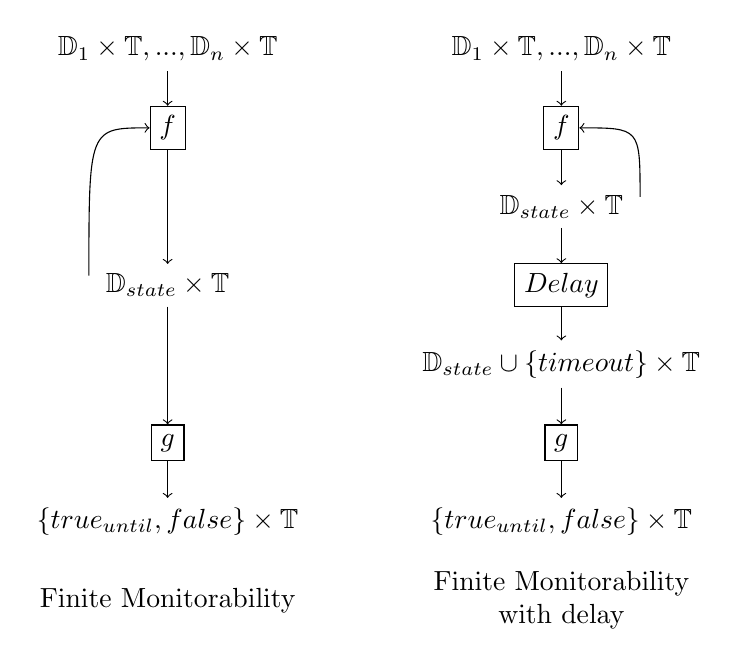
\begin{tikzpicture}
			\node[] (inputRight){$\mathbb{D}_1\times\mathbb{T}, ..., \mathbb{D}_n\times\mathbb{T}$};
			\node[draw, below of=inputRight] (fRight){$f$};
			\node[below of=fRight] (stateRight){$\mathbb{D}_{state}\times\mathbb{T}$};
			\node[draw, below of=stateRight] (delayRight){$Delay$};
			\node[below of=delayRight] (stateDelayRight){$\mathbb{D}_{state}\cup\{timeout\}\times\mathbb{T}$};
			\node[draw, below of=stateDelayRight] (gRight){$g$};
			\node[below of=gRight] (outputRight){$\{true_{until}, false\}\times\mathbb{T}$};
			
			\draw[->] (inputRight) -- (fRight);
			
			\node[right of = stateRight] (ha){};
			\node[right of = fRight] (hb){};
			\draw[->] (ha)  .. controls (hb) .. (fRight);
			
			\draw[->] (fRight) -- (stateRight);
			\draw[->] (stateRight) -- (delayRight);
			\draw[->] (delayRight) -- (stateDelayRight);
			\draw[->] (stateDelayRight) -- (gRight);
			\draw[->] (gRight) -- (outputRight);
			\node [below of=outputRight, align=center] (h0){Finite Monitorability\\with delay};

			
			\node[left of = inputRight] (h1){};
			\node[left of = h1] (h2){};
			\node[left of = h2] (h3){};
			\node[left of = h3] (h4){};
			
			\node[left of = h4] (inputLeft){$\mathbb{D}_1\times\mathbb{T}, ..., \mathbb{D}_n\times\mathbb{T}$};
			\node[draw, below of=inputLeft] (fLeft){$f$};
			\node[below of = fLeft] (h5){};
			\node[below of=h5] (stateLeft){$\mathbb{D}_{state}\times\mathbb{T}$};
			\node[, below of=stateLeft] (delayLeft){};
			\node[draw, below of=delayLeft] (gLeft){$g$};
			\node[below of=gLeft] (outputLeft){$\{true_{until}, false\}\times\mathbb{T}$};
			\draw[->] (inputLeft) -- (fLeft);
			\draw[->] (fLeft) -- (stateLeft);
			\draw[->] (stateLeft) -- (gLeft);
			\draw[->] (gLeft) -- (outputLeft);
			
			\node[left of = stateLeft] (hc){};
			\node[left of = fLeft] (hd){};
			\draw[->] (hc)  .. controls (hd) .. (fLeft);
			
			\node [below of=outputLeft] {Finite Monitorability};
		\end{tikzpicture}
		\centering
		\caption{Overview Finite Monitorability - with or without \emph{delay}}
		\label{fig:OverviewMonitorability}
	\end{figure}
	\subsection{Finite Monitorability}
		%TODO mention figure
		For the definitions of streams and functions defined on them, TeSSLa-like syntax is used. Also, some standard TeSSLa functions are used in the definitions. 
		\subsubsection{Input Streams}
			Let $S_1, S_2, ..., S_n$ be input streams with\\
			$\forall i:$ $S_i=(\mathbb{T}\cdot \mathbb{D}_i)^\omega\cup(\mathbb{T}\cdot \mathbb{D}_i)^+\cup(\mathbb{T}\cdot \mathbb{D}_i)^*\cdot(\mathbb{T}_\infty\cup\mathbb{T}\cdot\{\bot\})$ and\\
			All types $D_i$ have a finite size.
		\subsubsection{State Stream}
			\label{monitorability_state}
			Let $S_{state}$ with\\
			$S_{state}= (\mathbb{T}\cdot \mathbb{D}_{state})^+\cup(\mathbb{T}\cdot \mathbb{D}_{state})^*$\\
			be a state stream, where $\mathbb{D}_{state}$ has a finite size.\\
			Further let $f: S_1 \times S_2 \times ... \times S_n \times S_{state}\rightarrow S_{state}\times \mathbb{T}$ a state transition function, which defines the state stream in an incremental fashion:\\
			$\forall t\in \mathbb T \exists i\in \{1,2,...,n\}: S_i(t)\in\mathbb D_i$\\
			$\rightarrow S_{state}(t)= f(S_1(t), S_2(t), ..., S_n(t), last(S_{state}, merge(S_1, S_2, ..., S_n))(t))$\\
			The runtime of $f$ is in $\mathcal{O}(1)$.
		\subsubsection{Output Stream}
			Let $S_{output}= (\mathbb{T}\cdot \{true_{until}, false\})^+\cup(\mathbb{T}\cdot \{true_{until}, false\})^*$\\
			be the output stream, which is defined via a function\\
			$g: \mathbb{D}_{state}\times \mathbb{T}\rightarrow \{true_{until}, false\}\times \mathbb{T}$\\
			The runtime of $g$ is in $\mathcal{O}(1)$.
		\subsubsection{Evaluation}
			A property of a set of streams is called \emph{Finite Monitorable}, if a function $f$ with type $\mathbb{D}_{state}$ and a function $g$ exist, which fulfill the characteristics called above, and which outputs $true_{until}$, as long as the property is fulfilled and $false$, in any other case. It should be noted that these definitions are \emph{timestamp conservative}, because the streams $S_{state}$ and $S_{output}$ can only change their data value at the timestamps of input events.
		% TODO transducer
		\subsubsection{Equivalences}
			
	\subsection{Finite Monitorability with Delay}
		%TODO mention figure
		Not all of the TADL2 constraints can be monitored in a \emph{timestamp conservative}. For example, the \emph{RepeatConstraint} with the attributes $lower=upper=4$ and $span=1$ expects subsequent events to have a time distance of $4$. If one event is missing, the output of a timestamp conservative monitor would still be $true_{until}$, until the next input event arrives. Therefore, the monitor cannot not check the constraint correctly. Because of this problem, the definition of \emph{Finite Monitorability} is expanded by the ability of introducing new timestamps. To ensure the finiteness of the monitor, only one new timestamp can be introduced, more on that in \ref{DelayGenerator}.
		\subsubsection{Input Streams}
			The definition of the input streams are unchanged.
		\subsubsection{State Stream}
			The function $f$ remains unchanged, but the state stream $S_{state}$ is expanded by an \emph{timeout} value, which is inserted after a specific period of time, in which no input event has arrived.
		\subsubsection{Delay}
			\label{DelayGenerator}
			A \emph{Delay Generator} is inserted into the definition. It has two tasks, first it copies each input it gets from the state transition function $f$ to its output. At the timestamp where an input is copied, a timer, which length depends on the state of the monitor, is started. If the next input comes before the timer runs out, the timer is resetted and started again. If the timer runs out, the Delay Generator outputs the $timeout$ signal, which is repeated at every following input. After the timer has run out once, it is not started again. 
		\subsubsection{Output Stream}
			The output function $g$ is expanded by the \emph{timeout} value:\\
			$g: (\mathbb{D}_{state}\cup\{timeout\})\times \mathbb{T}\rightarrow \{true_{until}, false\}\times \mathbb{T}$\\
			The definition of the output stream $S_{output}$ remains unchanged.
		\subsubsection{Evaluation}
			A property of a set of streams is called \emph{Finite Monitorable with Delay}, if a function $f$ with type $\mathbb{D}_{state}$, a delay generator and a function $g$ exist, which fulfill the characteristics called above, and which outputs $true_{until}$, as long as the property is fulfilled and $false$, in any other case.
			
	\subsection{Non-Finite Monitorability}
		Not all TADL2 constraints are finite monitorable, because a monitor would require infinite memory and/or time resources. In a theoretical view, this makes online monitoring on infinite traces impossible, because a machine with infinite resources does not exist in the real world. In a practical view, many of these problems are solved by using a system with finite memory, with the hope that this finite resources would be enough, to cover the inputs of the ''real world''. In these cases, a distinction is useful, as some constraints have resource requirements, that grow continuously with every input event. These constraints will be called \emph{always Non-Finite Monitorable}. Others constraints only require infinite resources in worst case scenarios, therefore these will be called \emph{worst case Non-Finite Monitorable}. Obviously, the constraints with continuous resource requirement growth cannot be monitored infinitely, but the constraints, that only need infinite resources, can be monitored in many cases.
		%TODO klassifizierung weiter ausführen

	 
  %!TEX root = thesis.tex
\chapter{Analysis of the Monitorability of the TADL2 Timing Constraints}
\label{chapter-TADL2}

\section{DelayConstraint}
\section{StrongDelayConstraint}
\section{RepeatConstraint}
\section{RepetitionConstraint}
\section{SynchronizationConstraint}
\section{StrongSynchronizationConstraint}
\section{ExecutionTimeConstraint}
\section{OrderConstraint}
\section{ComparisonConstraint}
\section{SporadicConstraint}
\section{PeriodicConstraint}
\section{PatternConstraint}
\section{ArbitraryConstraint}
\section{BurstConstraint}
\section{ReactionConstraint}
\section{AgeConstraint}
\section{OutputSynchronizationConstraint}
\section{InputSynchronizationConstraint}
  %!TEX root = thesis.tex

\chapter{Implementation}
\label{chapter-implementation}
	\section{Implementation of the TADL2 Constraints}
	In this chapter, the implementation of the monitor of each constraint will be explained. This is done by giving a short documentation of each monitor. Additionally, the worst-case memory usage and the worst case and average run time per event are shown. In section~\ref{sec:performance}, each monitor is run on traces, which were generated to match the constraints with specific parameters, to evaluate which performance can be expected in practical usage of the implementation.\\
	All implementations have in common that they consist of 2 or 3 sections, similar to the state transition, delay (if needed) and output as defined in chapter~\ref{chapter-monitorability}. These sections are the basis for the computational complexity analysis because the generated state defines the required memory capacity and the state transition function, the output function and the calculation of the required delay define the required time per timestamp with input events.\\
	The implementations are programmed and tested for version 1.2.2 of the TeSSLa interpreter.
\subsubsection{Output of the  monitors}
	The monitors output RV-LTL truth values ($\top, \bot, \top^p, \bot^p$), which are represented as two boolean variables. One of these variables is showing the truth value on the prefix, which was processed until this point in time. The other variable shows if the output possibly changes in upcoming timestamps. These two variables are packed inside of the type \textit{fourValuedBoolean}. The individual values are mapped in the following way: 
	\begin{table}[H]
		\begin{tabular}{|c|c|c|}
			\hline
			\textit{fourValuedBoolean.value} & \textit{fourValuedBoolean.final} & RV-LTL \\
			\hline
			true & true &  $\top$\\
			\hline
			true & false &  $\top^p$\\
			\hline
			false & false & $\bot^p$ \\
			\hline
			false & true &  $\bot$\\
			\hline
		\end{tabular}
		\centering
	\end{table}
	Additionally to the state of the monitor, the previous output of the monitor is stored. If the previous output was $\bot$, the new output of the monitor is ignored and the output stays $\bot$. This is done to simplify the state and state transition of the monitor. For example, in the \textit{OrderConstraint}, the number of events, which occurred in the input streams, are stored as state. In the individual input timestamps, the correct order of the events can be checked in combination with the previous output of the monitor. If the previous output is unknown, the state must be defined more complex.
	 
\subsection{DelayConstraint}
	The implementation of the \emph{DelayConstraint} monitor stores a list of $source$ events, which did not have a matching $target$ event yet as the monitors' state. This list is expanded by every $source$ event, which is appended at the end of the list. If a $target$ event occurs, all matching $source$ events (possibly none) are removed from the list. As stated in section~\ref{monitorability_DelayConstraint}, this list can grow infinitely long in worst-cases when the time domain is defined in an uncountable way. In these worst-cases, an infinite number of $source$ events may occur before any event can be removed from the list when a matching $target$ event occurs.\\
	The used TeSSLa version is using integer values as time domain. Therefore it is countable and the list cannot grow infinitely because at most $upper$ $stimulus$ events need to be stored and the largest possible length of the list is linear dependent on the parameter $upper$. Because this list is the only growable memory usage, the algorithm is in $\mathcal{O}(upper)$ in terms of memory.\\
	In timestamps with a $target$ event, all events in the list, which are in the right time distance, are removed from the list. In worst-cases, all events in the list must be checked and removed, which means the worst-case run time of the state transition is linear dependent on the length of the list and therefore is $\mathcal{O}(upper)$. %In normal cases, only a few or none events must be removed, which are in the beginning of the list. Therefore, a nearly constant time behaviour can be expected.\\
	The output function checks if the updated list of unmatched $source$ events is either empty or the event in the head of the updated list is not older than $upper$. In the first case, there is no $source$ event without a matching $target$ event. Therefore the output is $\top^p$. If the list is not empty and the entry in the head of the list is younger than $upper$, the constraint is currently unsatisfied, but a satisfying state can still be reached. In this case, the output is $\bot^p$. If the entry in the head of the list is older than $tolerance$, there cannot be a matching $target$ event. Therefore the output of the monitor is $\bot$. All these checks are done in constant time. Therefore the output function is in $\mathcal{O}(1)$.\\
	The required delay period is calculated by adding $upper$ to the timestamp of the head of the list of unmatched $source$ events, subtracted by the timestamp of the current event ($\mathcal{O}(1)$).
	
\subsection{StrongDelayConstraint}
	The \emph{StrongDelayConstraint} is implemented very similarly to the \emph{DelayConstraint}. The only difference in the state transition is that exactly one event, which is the head of the list of unmatched $source$ events, is removed when a matching $target$ event occurs. Therefore, the maximal memory usage is the same ($\mathcal{O}(upper)$), but the run time of the state transition is constant per input timestamp because only the head of the list has to be considered in the transition.\\
	The output function is nearly the same as in the previous constraint. The only difference is that in timestamps containing $target$ events, it is checked if this event has a $source$ event in the right distance. If not, the output is $\bot$. This check is also done in constant time. Therefore the output function still is in $\mathcal{O}(1)$. The calculation of the delay period remains unchanged.
	
\subsection{RepeatConstraint}
	The implementation of the \emph{RepeatConstraint} stores the timestamps of the $span+1$ previous events as the state in a list. At every event, its timestamp is appended to the previous tail of the previous list if already more than $span$ events occurred. If less than $span$ events occurred before this timestamp, the timestamp is added to the entire list, not to the tail. The runtime for appending to the list is constant and the list is at most $span+1$ items long.\\
	The required delay period is calculated by adding $upper$ to the  $span^{th}$ oldest event (or the first event, if there have been less than $span$ events before) minus the current timestamp. Again, this is done in constant time because the timestamps required for this calculation are the first or second in the list.\\
	The output function checks if the $span^{th}$ oldest event is not older than $upper$ and not younger than $lower$. If there have not been $span$ events before, it is checked if the first event is not older than $upper$. If this property is fulfilled, the output is $\top^p$ and in any other case, it is $\bot$. Like in the calculation of the required delay period, the run time is constant. Therefore, the entire implementation is in $\mathcal{O}(span)$ in terms of memory and in $\mathcal{O}(1)$ in terms of time per event.
	
\subsection{RepetitionConstraint}
	The  \emph{RepetitionConstraint} is defined as\\[10pt]
		$RepetitionConstraint(s, lower, upper, span, jitter)$\\
		$\equiv \exists X\subset \mathbb{T}: RepeatConstraint (X, lower, upper, span)$\\
		\hspace{7cm}$\land$ $StrongDelayConstraint(X, s, 0, jitter)$\\[10pt]
	The implementations of the \emph{Repeat-} and the \emph{StrongDelayConstraint} cannot be used to implement this constraint because the timestamps of $X$ are unknown.\\
	Relevant for the monitoring are the upper and lower bounds of the elements of $X$, which precede the actual events in the event stream $s$. The bounds are stored as two lists with the length of $span$. One list contains the lower bounds for the next $span$ $X$, and the other list contains the upper bounds. At every input event, the new boundaries for the $span^{th}$ next $X$ are calculated, the lower bound by $max(List\_head(last(LowerBoundX, e)), time(e)-jitter)$ and the upper bound by $min(List\_head(last(UpperBoundX, e)), time(e))$. These new boundaries are appended to the end of the lists, while the oldest entries in the lists' head are removed. These two lists with the size of $span$ are the only growing storage. Therefore the algorithm is in $\mathcal{O}(span)$ in terms of memory. The run time of the state transition function is constant (removing the lists head and appending an entry to the lists).\\
	The output function checks if the current timestamp is between the lower bound for the current timestamp of $X$ and $jitter$ behind the upper bound for that value. If this is the case, the output is $\top$. In any other case, it is $\bot$. Because the upper and lower bound for the current $X$ value can be directly accessed (they are the head of the lists), the output function is in $\mathcal{O}(1)$.
	
\subsection{SynchronizationConstraint}
	The \emph{SynchronizationConstraint} is defined via an application of the \emph{DelayConstraint}, but the application uses a set of unknown timestamps($\exists X: ...$). Therefore the \emph{DelayConstraint} cannot be used for the implementation of this constraint.\\
	Because TeSSLa does not allow to define macros or functions with a variable number of input streams, events of each input timestamp must be placed into an integer list, which contains the index (starting at 1) of all streams, which have an event in this timestamp. This list is then used as a parameter for the implementation. The creation of this list is already implemented for up to 10 streams.\\
	The implementation of the \emph{SynchronizationConstraint} stores all events that occurred not longer than $tolerance$ ago in a list. In each entry, this list contains the stream in which the event occurred, the timestamp of the event occurrence and a boolean variable that expresses if a fulfilled synchronization cluster for this event has already been found.\\
	This list is updated in every input timestamp in three steps. First, each event occurrences in this timestamp are appended to this list. Second, the list is separated into two parts, one with the events older and one with the events younger than $tolerance$. The part of old events is still stored in this timestamp but removed after it. The younger events form the state that is stored for the next event occurrences. Third, it is checked if at least one event of every stream is part of the list of younger events. In this case, a fulfilled synchronization cluster has been found and the boolean variable that states if a synchronization cluster is found for this event is set to $true$ for all events in this list.\\
	Like in the \emph{DelayConstraint}, this list can grow infinitely when the time domain is uncountable, which is not the case in the used TeSSLa version. Because the TeSSLa uses integers as time domain, at most $|event|\footnote{|event| is the number of streams, not the number of events.}*tolerance$ events can occur in the $tolerance$ interval. Therefore, the algorithm is in $\mathcal{O}(|event|*tolerance)$ in terms of memory. The first step of the state transition is in $\mathcal{O}(|event|*tolerance)$ because at most $|event|$ events must be appended to the list and the list has the maximum length $tolerance$. In worst cases, every event in the list(which is in ascending order) is older than tolerance. Therefore, the worst-case runtime of the separation in the second step of the state transition is in $\mathcal{O}(|event|*tolerance)$ in terms of time. In the third step, the complete stored list of young events must be examined to check if the cluster is fulfilled and, if needed, every event in the list must be set to fulfilled. Therefore the third step is in $\mathcal{O}(|event|*tolerance)$ in terms of time.\\
	The output function checks first if there are any entries in the list of stored events, which were not part of a synchronization cluster yet. If this is not the case, the output is $\top^p$, because there are no unsatisfied synchronization clusters in this case. If there are entries without a synchronization cluster so far, it is checked if all list entries, which were removed in this timestamp (and therefore are older than $tolerance$), had a synchronization cluster. If one of these removed entries did not have a synchronization cluster, the constraint is unsatisfied and the output is $\bot$. If all of them were part of at least one cluster, the output is $\bot^p$, because there are still entries without cluster in the list (see first check), but they still can be satisfied. Because the list can have the size $|event|*tolerance$ and all of the entries are considered in the first check of the output function, the output function is in $\mathcal{O}(|event|*tolerance)$ in terms of time.\\
	The required delay is calculated by adding $tolerance$ to the timestamp of the oldest stored unsatisfied event, subtracted by the timestamp of the current timestamp. The list is in ascending order, but the only unsatisfied events are relevant for the delay, which means the entire list must be checked in worst cases. Therefore, the calculation of the required delay is in $\mathcal{O}(|event|*tolerance)$.
	
\subsection{StrongSynchronizationConstraint}
	The \emph{StrongSynchronizationConstraint} is defined as an application of the \emph{StrongDelayConstraint}, but this application cannot be used for the implementation, like in the previous constraint.\\
	Similar to the implementation of the \emph{SynchronizationConstraint}, the events of each timestamp must be merged into a list containing the indices of the streams, which contain the events.\\
	The difference between the \emph{Synchronization-} and the \emph{StrongSynchronizationConstraint} is that each event is part of exactly one synchronization cluster in the \emph{StrongSynchronizationConstraint}. Therefore, the implementation is different from the implementation of the previous constraint. Not every event is stored separately, but information about synchronization clusters, containing their start time and in which stream an event occurred in this cluster, is stored.\\
	The information of which the state consist is stored in a list of synchronization clusters. The list entries consist of a time expression containing the latest possible start point of the cluster and a map. This map has one entry for every input stream and uses the indices of the streams as keys and boolean variables as values. The map shows which of the streams already had an event in this synchronization cluster.\\
	For the state transition, every event occurring in this timestamp is either inserted into an existing cluster or a new cluster is appended at the end of the list. Two conditions must be fulfilled to insert an event into a cluster. First, the cluster must not be older than upper. Second, the boolean variable in the map entry of this stream must be $false$, which shows that there was no event of this stream in this cluster before. If these conditions are not fulfilled for all existing clusters, a new cluster is created and appended at the end of the list. This ensures that the list is always in chronological order.\\
	For the search of a matching cluster, each entry of the list is considered in worst-cases. Therefore the run time of this part of the state transition is linear to the number of active clusters. In worst-cases, this number is $tolerance$ when one event occurs in every timestamp in always the same stream.\\
	In the second step of the state transition, it is checked for every stored cluster if it is fulfilled. If so, it is removed from the list. To check, if a cluster is fulfilled, one boolean check must be done for every input stream, therefore at most boolean $tolerance*|event|$ checks must be done and the worst-case run time of the state transition is in $\mathcal{O}(tolerance * |event|)$. When the events occur in timewise separated synchronization clusters, the list is significantly shorter than $tolerance$ and the run time can be expected to be linear to the number of input streams.\\
	The list storing the clusters is at most $tolerance$ long and the size of individual entries of the list is linear dependent on the number of streams because they store a boolean variable for every stream. Because of these length restrictions of the list, the algorithm is in $\mathcal{O}(|event|*tolerance)$ in terms of memory.\\
	The output function checks first if the list of stored synchronization clusters is empty. If this is the case, the output is $\top^p$, because there are no unsatisfied synchronization clusters. If the list is not empty, it is checked if the oldest unsatisfied cluster, which is always in the head of the list, is younger than $tolerance$. If so, the output is $\bot^p$, because the constraint is unsatisfied but can be satisfied with upcoming events. If the oldest cluster is older than tolerance, the constraint is unsatisfied and cannot be satisfied with upcoming events, therefore the output us $\bot$. All these checks are done in constant time. The required delay is calculated by adding $tolerance$ to the timestamp of the oldest stored unsatisfied cluster, subtracted by the timestamp of the current timestamp ($\mathcal{O}(1)$).
	
\subsection{ExecutionTimeConstraint}
	The implementation of the \emph{ExecutionTimeConstraint} is using TeSSLa's \emph{runtime} operator on the \emph{start} and \emph{stop} events, which calculates the absolute runtime without any interruptions. The time of interruptions is also calculated by this operator and then summed up. The sum of these interruptions is reset at every $start$ event. For the calculation of this sum with resets, a macro called \textit{resetSum} was programmed, which is a modified version of TeSSLas \textit{resetCount} operator.\\
	TeSSLa's \emph{runtime} operator subtracts the timestamps of the events of the second parameter (in this case \emph{stop} and \emph{resume}) from the timestamps of the events of the first parameter(\emph{start} and \emph{preempt}). Therefore it stores the timestamps of the \emph{start} and \emph{preempt} events are stored, additionally to the sum of the preemptions.
	For the output, the runtime can be calculated by subtracting the second application (with $preempt$ and $resume$ as parameters) of TeSSLa's $runtime$ operator from the sum of the first applications (with $start$ and $stop$ as parameters) of this operator. If the runtime should be checked in timestamps without a \emph{stop} event, the second parameter of the first application of the $runtime$ operator must be replaced by a current event. In the implementation, this is done by merging all input streams and the delay stream.\\
	The resulting runtime must be smaller or equal to $upper$ at any point of time and greater or equal to $lower$ at \emph{stop} events. If this is the case, the output is $\top^p$, in any other case, it is $\bot$. The required delay is calculated by subtracting the runtime so far from upper. All of these operations are simple arithmetic functions on timestamps. Therefore the algorithm is in $\mathcal{O}(1)$ in terms of time. The required storage space is fixed. Therefore it is also in $\mathcal{O}(1)$ in terms of memory.

\subsection{OrderConstraint}
	The implementation counts the number of events in the $source$ and $target$ stream and stores these numbers as the monitors state. This update is done in constant time and the required storage space is also constant. The output function compares the number of $source$ and $target$ events. If the number is equal, the constraint is fulfilled until this point in time and the output is $\top^p$. If the number $source$ events is larger, the constraint is unsatisfied but can be satisfied with upcoming events. Therefore $\bot^p$ is the output. If the number of $target$ events is larger, the order of the events is invalid, the constraint is unsatisfied and cannot be satisfied anymore. Therefore, the output is $\bot$ in these cases. The checks of the output function are also done in constant time.\\
	The introduction of new timestamps is not required for this constraint. Therefore no delay period must be calculated.
	
\subsection{ComparisonConstraint}
	The \emph{ComparisonConstraint} defines comparisons between timestamps. These functionalities are already defined in TeSSLa. Therefore no implementation is given as part of this thesis.  
	
\subsection{SporadicConstraint}
	The \emph{SporadicConstraint} is defined as an application of the \emph{Repetition-} and the \emph{RepeatConstraint}. Therefore the \emph{SporadicConstraint} is also implemented as an application of them. The implementations of the \emph{Repetition-} and the \emph{RepeatConstraint} are both in $\mathcal{O}(span)$ in terms of time and memory. Because $span$ is fixed to 1 in the \textit{SporadicConstraint}, the implementation is in $\mathcal{O}(1)$ in terms of memory and time.
	
\subsection{PeriodicConstraint}
	The \emph{PeriodicConstraint} is defined as an application of the \emph{SporadicConstraint} and is also implemented like this. Because the \emph{SporadicConstraint} is in $\mathcal{O}(1)$ in terms of memory and time, the \emph{PeriodicConstraint} is also.
	
\subsection{PatternConstraint}
	The \emph{PatternConstraint} is defined as an application of the \emph{Periodic-}, \emph{Delay-} and \emph{RepeatConstraint}. Because of the set of unknown timestamps $X$, the \emph{Periodic-} and \emph{DelayConstraint} cannot be used for the implementation. The set $X$ is not used in the application of the \emph{RepeatConstraint}. Therefore its implementation is used as part of the output function.\\
	The implementation of the \emph{RepeatConstraint} is in $\mathcal{O}(span)$ in terms of time memory. The $span$ attribute is set to 1 in the application. Therefore the run time and memory usage are constant in this part.\\
	In the implementation of the \emph{PatternConstraint}, the lower and upper bound for the current timestamp of $X$ is stored. At every event, these bounds are further enclosed, taking the previously known bounds and the bounds implied by the current event
	\begin{align}
		x\in X: &time(event)-\text{\emph{offset}}_{count(event)\text{ mod }|\text{\emph{offset}}|}-jitter \leq x\\
			     &\leq  time(event)-\text{\emph{offset}}_{count(event)\text{ mod }|\text{\emph{offset}}|}
	\end{align}
	into account. The new lower bound is set by using the maximum of the previous lower bound and the lower bound implied by the current event, the new upper bound by using the minimum of the previous upper bound and the upper bound implied by the current event. At every $|\text{\emph{offset}}|^{th}$ event, $period$ is added to the current bounds. The access of the map entries is done in constant time. Therefore the calculation of these new borders is also done in constant time and the state transition function in $\mathcal{O}(1)$ in terms of time.\\
	The output function checks if the timestamp of the current event is between the lower bound plus $\text{\emph{offset}}_{count(event)\text{ mod }|\text{\emph{offset}}|}$ and the upper bound plus \\$\text{\emph{offset}}_{count(event)\text{ mod }|\text{\emph{offset}}|}$ plus $jitter$. If so, the output is $\top^p$, if not, it is $\bot$. The previously defined output is conjuncted with the output of the application of the \textit{RepeatConstraint}. The comparisons of timestamps are done in constant time and monitoring the \textit{RepeatConstraint} with $span=1$ if likewise. Therefore, the output function is in $\mathcal{O}(1)$.\\
	The required delay is defined by the time distance between the current timestamp and the upper bound for X, plus the expected offset of the following event, plus the allowed deviation ($jitter$).\\
	The only state stored in the implementation are the upper and lower bound for the  current $x$-value. Therefore the implementation itself is in $\mathcal{O}(1)$ in terms of memory, but the size of the \textit{offset}-parameter, which is a map, is not limited in size and the complete algorithm, including the parameters, is $\mathcal{O}(|\text{\textit{offset}}|)$ in terms of memory.
	
\subsection{ArbitraryConstraint}
	The \emph{ArbitraryConstraint} is defined as multiple applications of the \emph{RepeatConstraint} and is also implemented this way. The number of applications of the \emph{RepeatConstraint} is dependent on the number of elements in the $minimum$ and $maximum$ parameters. The runtime of the \emph{RepeatConstraint} is in $\mathcal{O}(1)$ per application and event. Therefore the \emph{ArbitraryConstraint} is in $\mathcal{O}(|minimum|)$ in terms of time. The memory usage of the \emph{RepeatConstraint} is in $\mathcal{O}(span)$. In the application of the \emph{RepeatConstraint}, the $span$ parameter increases for each of the $|minimum| = |maximum|$ applications. Therefore, the implementation is in $\mathcal{O}(\sum_{i=1}^{|minimum|}i)\widehat{=}\mathcal{O}(|minimum|^2+|minimum|)$ in terms of memory.

\subsection{BurstConstraint}
	The \textit{BurstConstraint} is defined as a twofold application of the \emph{RepeatConstraint} and is also implemented this way. The \textit{RepeatConstraint} is in $\mathcal{O}(span)$ in terms of memory and in $\mathcal{O}(1)$ in terms of time. Because the $span$ attribute is set to 1 and $maxOccurrences$ in the applications of the \textit{RepeatConstraint}, the implementation of the \emph{BurstConstraint} is in $\mathcal{O}(maxOccurrences)$ in terms of memory and in $\mathcal{O}(1)$ time.

\subsection{ReactionConstraint}
	The correctness of the \textit{EventChain} is assumed in the implementation. If this property is unknown, it must be checked individually.\\
	The implementation of the \emph{ReactionCostraint} stores a map, which maps the color of $stimulus$ events, which did not have a matching $response$ event yet, to their timestamps. This state is updated at every input event. $Stimulus$ events are inserted into the map, $response$ events remove, if possible, an event from the map called above. Similar to the \emph{DelayConstraint}(the \emph{ReactionCostraint} can be seen as an extension of the \emph{DelayConstraint}, that additionally considers the color of events), the maximal number of entries in the map is the maximal number of $stimulus$ events that could possibly occur in an interval of the length $maximum$, which is $maximum$.  Therefore, the algorithm is in $\mathcal{O}(maximum)$ in terms of memory. The state transition (insertion, lookup and possibly remove in a map) is in $\mathcal{O}(1)$ in terms of time.\\
	The required delay is calculated by adding $maximum$ to the timestamp of the oldest entry in the map mentioned above and subtracting the current timestamp. Because the map is unsorted, every entry of the map must be considered for this. Therefore, the calculation of the required delay is in the time complexity class $\mathcal{O}(maximum)$.\\
	The output function first checks if the map of unmatched $stimulus$ events is empty. If so, the constraint is satisfied and the output is $\top^p$. If there are entries in the map and the oldest entry is older than $tolerance$, the constraint is unsatisfied and cannot be satisfied by upcoming events. In this case, the output is $\bot$. If the oldest entry is younger than $tolerance$, the constraint is currently unsatisfied but can be satisfied by upcoming events. Therefore, the output is $\bot^p$. To find the oldest entry in the map, all entries must be considered. Therefore, the output function is linear dependent on the size of this map, which is at most $maximum$.
	
\subsection{AgeConstraint}
	Like before, the correctness of the \textit{EventChain} is assumed in the implementation. If this property is unknown, it must be checked individually.\\
	Similar to the implementation of the \emph{ReactionCostraint}, the \emph{AgeConstraint} monitor stores a map containing the latest $stimulus$ event, which is younger than \textit{maximum}. The $color$ value is used as map key and the timestamp is used as map value. This map has the maximum size $maximum$ and is updated at every input event. $Stimulus$ events are inserted or updated, and entries that are older than $maximum$ are removed. To make this update faster, a list containing the colors of the events in the map is stored additionally. The maximal size of this list is also $maximum$ and the colors are stored in chronological order so that the color that occurred the longest time ago is in the head of the list. The update is done by looking at the head of the list and removing this entry from the list and the corresponding entry with the same color from the map if the entry is older than $maximum$. These operations are done in constant time but need to be repeated, as long as the color in the head of the map is too old, so at most $maximum$ times. Inserting or updating the $stimulus$ event to the map is done in constant time, but inserting or updating the list requires to remove any previous entry with the color of the current event. For this, every entry in the map has to be processed, which means this operation takes $maximum$ steps in worst-cases. Consecutively, the state and the state transition are in $\mathcal{O}(maximum)$ in terms of memory and time. The creation of new timestamps is not needed in this constraint because only previous events need to be considered, upcoming events not.\\
	In timestamps containing a $response$ event, the output function checks if a $stimulus$ event with the same color is in the map and if the time distance between them is greater or equal to $minimum$ and smaller or equal to $maximum$. If so, the output is $\top^p$. If not, it is $\bot$. Timestamps without $response$ events cannot lead to a violation of the constraint. The lookup in the map and the comparisons are done in constant time.

\subsection{OutputSynchronizationConstraint}
	Similar to the \emph{Synchronization-} and \emph{StrongSynchronizationConstraint}, the input streams cannot be directly used as a parameter. For the \emph{OutputSynchronizationConstraint}, a stream of maps must be created, representing the events of each timestamp. The key of each entry is the index of the stream (0 for the $stimulus$ stream, 1, 2, ... for the \textit{response} streams), in which the event occurred and the value is the color of the event. Again, the creation of this map is already implemented for up to 10 $response$ streams.\\
	In the \emph{OutputSynchronizationConstraint}, there must be one synchronization cluster of the length $tolerance$ for each $stimulus$ event. Each $response$ stream must have at least one event of the same color as the $stimulus$ event in this cluster. There is no time distance between this cluster and the $stimulus$ event defined.\\
	The implementation of the \emph{OutputSynchronizationConstraint} is storing three different information as the state of the monitor. First, a set of the stimulus colors, which did not have a $response$ event in the same color yet. This set is updated at every input event, the color of $stimulus$ events is inserted and the colors of the $response$ events in the current timestamp are removed from the set. These updates are done in constant time. In worst-cases, where no matching $response$ events occur, the required storage space is linear depending on the number of $stimulus$ events.\\
	The second information is a map containing information about all synchronization clusters that were not finished before this point in time. This map is using the color attribute as key and the start timestamp and a map as value. This inner map uses the indices of the \textit{response} streams as keys and a boolean variable as value. This value shows whether there was an event for this synchronization cluster in this stream or not. This map is updated at every $response$ event. For each of these $response$ events, it is checked if a synchronization cluster with a matching color exists. If not, a new synchronization cluster with the color of the event is created if the color of this event was in the set of stimulus colors of the previous timestamp. The check per event (two lookups in maps, one in a set) is done in constant time. Therefore the entire update of this map is in $\mathcal{O}(|response|)$ in terms of time per input timestamp. In worst-cases, each event results in creating of a new synchronization cluster, which must be stored at least for the length of $tolerance$. The size of each information about one synchronization cluster is linear dependent on the number of $response$ streams and in each interval of the length $tolerance$, $tolerance*|response|$ events can occur and create a new synchronization cluster. Therefore this information is in $\mathcal{O}(tolerance*|response|^2)$ in terms of memory.\\
	The third stored information is similar to the second, but the clusters that are either older than tolerance or fulfilled are removed from the map. Therefore, the worst-case memory consumption is also $\mathcal{O}(tolerance*|response|^2)$. To remove fulfilled clusters, it is checked for each cluster in the map if there was at least one event in each $response$ stream of the color of the cluster. Therefore, this update is in $\mathcal{O}(tolerance*|response|^2)$ in terms of time.\\
	In combination, the run time of the state transition is in $\mathcal{O}(tolerance*|response|^2)$ and the memory usage is in $\mathcal O(count(stimulus) + tolerance*|response|^2)$.\\
	The required delay is calculated by adding $tolerance$ to the start time of the oldest unfinished cluster and subtracting the current timestamp. To get the oldest unfinished synchronization cluster, all map currently active clusters must be considered, which means the run time is linear dependent on the number of currently active clusters (at most $tolerance*|response|$).\\
	The output function checks first if the set of unmatched \textit{stimulus} and the map of stored synchronization clusters are empty. If this is the case, not \textit{stimulus} events had a fulfilled synchronization and the constraint is fulfilled until this point in time. The output is $\top^p$. If the set or the map is not empty, it is checked if all synchronization clusters are younger than $tolerance$. If so, the constraint is currently unsatisfied but can be satisfied by future events. In this case, the output is $\bot^p$. If the oldest synchronization cluster is older than $tolerance$, the constraint is unsatisfied and no future events can change this. Therefore, the output is $\bot$ in this case. The first check is done in constant time, and the second check requires considering each stored synchronization cluster. Therefore, the run time of the output is linear dependent on the number of stored events, which is at most $tolerance*|response|$.
	
%	The implementation of the \emph{OutputSynchronizationConstraint} is storing four different informations as state. First, a list of every color that occurred in $stimulus$. This is updated at every $stimulus$ event by appending its color to the list(run time: $\mathcal{O}(1)$, memory: $\mathcal{O}(count(stimulus))$).\\
%	Second, a map is stored, which is containing information about all synchronization clusters that were not finished before this point in time. This map is using the color attribute as key and the start timestamp and a map as value. This inner map uses the indices of the \textit{response} streams as keys and a boolean variable as value. This value shows, whether there was an event for this synchronization cluster in this stream or not. This map is updated at every $response$ event. For each of these $response$ events, it is checked, if a synchronization cluster with a matching color exists, if not, a new synchronization cluster with the color of the event is created. The check per event (two lookups in maps)  is done in constant time, therefore the entire update of this map is in $\mathcal{O}(|response|)$ in terms of time per input timestamp. In worst cases, each event results in the creation of a new synchronization cluster, which must be stored at least for the length of $tolerance$. The size of each information about one synchronization cluster is linear dependent on the number of $response$ streams and in each interval of the length $tolerance$, $tolerance*|response|$ events can occur and create a new synchronization cluster, therefore this information is in $\mathcal{O}(tolerance*|response|^2)$ in terms of memory. 
%	The third stored information is similar to the second, but the clusters that are either older than tolerance or fulfilled are removed from the map. Therefore, the worst case memory consumption is the also $\mathcal{O}(tolerance*|response|^2)$. To remove fulfilled clusters, it is checked for each cluster in the map, if there was at least one event in each $response$ stream of the color of the cluster. Therefore, this update is in $\mathcal{O}(tolerance*|response|^2)$ in terms of time.
%	The fourth stored information is a set of all colors that had a fulfilled synchronization cluster in the $response$ streams until this point in time. Inserting items into the set is done in constant time. The number of fulfilled synchronization clusters is at most the number events in all $response$ streams, divided by the number of the $response$ streams. Therefore, the required memory of this information is in $\mathcal{O}\left(\frac{\sum_i count(response_i)}{|response|}\right)$.\\
%	The combined time complexity class is $\mathcal{O}(tolerance*|response|^2)$. The combined memory complexity classes, which defines the memory complexity of the algorithm, is $\mathcal{O}\left(count(stimulus)+\frac{\sum_i count(response_i)}{|response|}+tolerance*|response|^2\right)$.\\
%	The required delay is calculated by adding $tolerance$ to the start time of the oldest unfinished cluster and subtracting the current timestamp ($\mathcal{O}(tolerance*|response|^2)$).\\
%	The output function checks that all stored synchronization clusters are either younger than $tolerance$ or fulfilled.
%	Because the entries of the map, that stores the synchronization clusters, cannot be accessed in way, that is sorted by age, every entry of the map must be checked for its age (at most $tolerance*|response|$ checks). For every synchronization cluster that is older than $tolerance$, it must be checked, if this cluster is fulfilled. The check of a single cluster requires to check the boolean variables of each stream. Per timestamp, at most $|response|$ synchronization clusters can be started, therefore at most $response$ clusters grow older than $tolerance$ per timestamp. Therefore, the output function is in $\mathcal{O}(tolerance*|response|^2)$ in terms of time per input timestamp.\\
%	At the end of the observation, it must be checked, if each $stimulus$ event had a matching synchronization cluster. For each of the at most $count(stimulus)$ $stimulus$ colors, a lookup in a set must be done, therefore this check is in $\mathcal{O}(count(stimulus))$ and the complete output function, including the check at the end of observation, is in $\mathcal{O}(tolerance*|response|^2 + count(stimulus))$ in terms of time.



\subsection{InputSynchronizationConstraint}
	The input streams must be transformed into a $map[Int, Int]$ stream, similar to the previous constraint, but this time the index 0 indicates the $response$ stream and the indices 1, 2, ... are indicating the $stimulus$ streams.\\
	The \emph{InputSynchronizationConstraint} is defined very similar to the \emph{OutputSynchronizationConstraint}. The difference is that the synchronization occurs in a set of $stimulus$ events, not in $response$ events.\\
	Despite the similarities, the implementation of the \emph{InputSynchronizationConstraint}  is different from the implementation of the \emph{OutputSynchronizationConstraint}. As the monitors state, a map that uses the numbers 1 to $|stimulus|$ as keys and as values a second map that uses colors (integer) as key and the timestamp of the latest occurrence of this color in the stream as value. This map is updated at every $stimulus$ event, at which either the timestamp of the latest occurrence of this color in this stream is updated, or a new inner map entry is created for this color.  The lookup, if there already is a matching entry in the map for this color in this stream and possibly its update is done in constant time, but the time for initializing a new entry is linear dependent on the number of $stimulus$ streams. Because $|stimulus|$ events may occur and introduce a new color in each timestamp, the state transition is in $\mathcal{O}(|stimulus|^2)$ in terms of time. The worst-case memory size of this information is in $\mathcal{O}(|stimulus|*count(stimulus))$ because the map described above possibly stores every input event of the $stimulus$ streams when they introduce a new color and therefore, a new entry in the inner map of the stream must be created. $Response$ events are not considered for the state of the monitor.\\
	The creation of new timestamps is not needed in this constraint because only previous events need to be considered. Therefore, the calculation of a delay span is not required.\\
	In timestamps containing a $response$ event, the output function checks if the last occurrences of the corresponding color in the $stimulus$ stream form a valid synchronization cluster. This is done by searching the youngest and oldest event with this color in the map of the latest $stimulus$ events. If an event of this color is missing, the age is interpreted as $\infty$ or $-\infty$, which leads to a length of the synchronization cluster that is definitely longer than $tolerance$. If the synchronization cluster is longer than $tolerance$, the constraint is violated and the output is $\bot$. If the cluster is not longer than $tolerance$, the output is $\top^p$. In timestamps without a $response$, the output remains unchanged. Because the color value is the key of the inner map, the time for searching the oldest and youngest event of this color is linear to the number of $stimulus$ streams. Therefore, the output function is in $\mathcal{O}(|stimulus|)$ in terms of time.
	
\subsection{EventChain}
	Additionally to the 18 TADL2 timing constraints, a monitor, which checks the correctness of \textit{EventChains} was implemented. An \textit{EventChain} is defined on a $stimulus$ and a $response$ stream as\\[10pt]
	$\forall x \in stimulus:\forall y\in response: x.color=y.color\Rightarrow x<y$\\[10pt]
	As a state, a set containing all colors that previously occurred in $reponse$ is stored. This set is updated at each $response$  event by an insertion into a set ($\mathcal{O}(1)$). The maximal size of this map is the number of events in $response$. Therefore the state is in $\mathcal{O}(count(response))$ in terms of memory.\\
	The output function checks if the color of every occurring $stimulus$ event is not in the set of $response$ colors, which is checked in constant time. If the color is in the set of $response$ colors, the output is $\bot$. Otherwise, it is $\top^p$.
	
\section{Conclusion}
Table~\ref{tab:complexityClasses} gives an overview of the worst-case memory consumption and the worst-case run time per input timestamp. The worst-case memory requirement and the runtime per input timestamp of the \textit{Repeat-}, \textit{Repetition-}, \textit{ExecutionTime-}, \textit{Sporadic-}, \textit{Periodic-}, \textit{Pattern-}, \textit{Arbitrary-} and \textit{BurstConstraint}, which are the \textit{simple monitorable} constraints, is either constant, or they are only limited by the parameters of the constraint, not by the input traces. The implementations of the \textit{Delay-}, \textit{StrongDelay-}, \textit{Synchronization-}, \textit{StrongSynchronization-}, \textit{Reaction-} and \textit{AgeConstraint} are limited by the events, which may occur in time intervals of a specific length. Monitoring the correctness of \textit{EventChains}, the \textit{OutputSynchronization-} or the \textit{InputSynchronizationConstraint} with these implementations require continuously growing memory resources and in the \textit{OutputSynchronizationConstraint}, the run time per input timestamp is continuously growing too. The implementation of the \textit{OrderConstraint} is in $\mathcal{O}(1)$ in terms of memory and time per event, although it is classified as \textit{Not simple monitorable}. This is because integers of a fixed length are used for the implementation of the constraint and only a finite subset of all streams that fulfill the constraint can be monitored correctly.

	\begin{table}
		\begin{tabular}{|c|c|c|}
			\hline
			& Memory & \makecell{Run Time per Input\\Timestamp} \\
			\hline
			{DelayConstraint} & $\mathcal{O}(upper)$ & $\mathcal{O}(upper)$ \\
			\hline
			{StrongDelayConstraint} &  $\mathcal{O}(upper)$ &  $\mathcal{O}(1)$ \\
			\hline
			{RepeatConstraint} & $\mathcal{O}(span)$ & $\mathcal{O}(1)$ \\
			\hline
			{RepetitionConstraint} & $\mathcal{O}(span)$ & $\mathcal{O}(1)$ \\
			\hline
			SynchronizationConstraint & $\mathcal{O}(|event|*tolerance)$ & $\mathcal{O}(|event|*tolerance)$ \\
			\hline
			StrongSynchronizationConstraint & $\mathcal{O}(|event|*tolerance)$ & $\mathcal{O}(|event|*tolerance)$ \\
			\hline
			ExecutionTimeConstraint & $\mathcal{O}(1)$ & $\mathcal{O}(1)$ \\
			\hline
			OrderConstraint & $\mathcal{O}(1)$ & $\mathcal{O}(1)$ \\
			\hline
			SporadicConstraint & $\mathcal{O}(1)$ & $\mathcal{O}(1)$ \\
			\hline
			PeriodicConstraint & $\mathcal{O}(1)$ & $\mathcal{O}(1)$ \\
			\hline
			PatternConstraint & $\mathcal{O}(1)$ & $\mathcal{O}(1)$ \\
			\hline
			ArbitraryConstraint & \makecell{$\mathcal{O}(|minimum|^2$\\$+|minimum|)$} & $\mathcal{O}(|minimum|)$\\
			\hline
			BurstConstraint & $\mathcal{O}(maxOccurrences)$ & $\mathcal{O}(1)$ \\
			\hline
			ReactionConstraint & $\mathcal{O}(maximum)$ & $\mathcal{O}(maximum)$ \\
			\hline
			AgeConstraint & $\mathcal{O}(maximum)$ & $\mathcal{O}(maximum)$ \\
			\hline
			OutputSynchronizationConstraint& \makecell{$\mathcal{O}(count(stimulus)$\\$+tolerance*|response|^2)$} &  \makecell{$\mathcal{O}(tolerance$\\$*|response|^2)$}\\
			\hline
			InputSynchronizationConstraint& \makecell{$\mathcal{O}(|stimulus|$\\$*count(stimulus))$} & $\mathcal{O}(|stimulus|^2)$ \\
			\hline
			EventChain & $\mathcal{O}(count(response))$ & $\mathcal{O}(1)$\\
			\hline
		\end{tabular}
		\centering
		\label{tab:complexityClasses}
		\caption{Worst-Case Run Times of the Implementations}
	\end{table}

	
	

  \subsection{Performance Analysis}

To get an overview of the capabilities of the monitor implementations, each of them were run on at least 100 traces with 1.000 events, which were randomly generated by following specific parameters to show, which of these parameters result in faster or slower run times. For this evaluation, the TeSSLa interpreter version 1.0.12 were used and it was run on a computer with a i5-6600k processor running on 4.3 GHz. The operating system was Windows 10.\\ %TODO excact windows version
The run times were measured as time between per event. For that, a program\footnote{This program and the complete measured run times can be found at \href{https://github.com/HendrikStreichhahn/TeSSLa-Autosar-Timing-Extensions/tree/master/traceGenerator}{https://github.com/HendrikStreichhahn/TeSSLa-Autosar-Timing-Extensions/tree/master/traceGenerator}} was written, which generates traces for each constraint and then measures the time between the input of the events of one timestamp and the output of the TeSSLa interpreter. The communication between the test program and the TeSSLa interpreter is done via the \textit{standard input} and \textit{standard output stream} of the interpreter. The time is measured by the java function \textit{System.nanoTime()} immediately before the events are written into the input stream and immediately after an reaction was received on the output stream. It must be noted, that this time measurement is not completely accurate, because neither the used java runtime environment, nor the operating system were build to fulfill real time requirements. Therefore, unpredictable delays may occur in the test program, in the java interpreter or between them, but the results show, what the monitors are capable of and where it limits are.\\
For every Trace, the minimum, the maximum and the average time per event was stored, additionally the overall minimum, overall maximum and overall average of the run times were determined.

\subsubsection{DelayConstraint}
	The \textit{DelayConstraint} was evaluated with 100 Traces of 1.000 events. The traces fulfilled the constraint with the attributes $lower\in\{100, 200, 300, 400, 500, 600, 700, 800, 900, 1000\}$ and $upper=lower$.  The distance of $source$ subsequent were $distance\in\{1, 2, 4, 16, 32, 64, 128, 256, 512, 1024\}$, while the distance was smaller than $2*lower$ in.  The run time per event was between 0.23ms and 55.3ms, averaging at 1.2ms per event. As expected, the highest average run times were by the traces with low event distances, because these traces require to store more timestamps. In table~\ref{tab:runtimeDelay} are the average run times for this constraint with the parameters $lower=upper=1000$ in dependency of the time between subsequent $stimulus$ events. It can be seen, that these differences are fairly small, because the trace generator does not create worst case traces for this constraint, where all stored $stimulus$ events must be removed in one one timestamp.
	\begin{table}
		\begin{tabular}{|c|c|c|c|c|c|c|c|c|c|c|c|}
			\hline 
			\makecell{Distance\\$stimulus$\\events}  & 	1	 & 2 	  & 4 	   & 8 	   & 16 	& 32 	 & 64 	  & 128    & 256 	& 512 	& 1024\\
			\hline
			\makecell{avg. run time\\per event(ms)}	& 1.92 & 1.95 & 1.72 & 1.4 & 1.21 & 1.12 & 1.08 & 0.94 & 0.95 & 1.02 & 1.08\\
			\hline
		\end{tabular}
		\centering
		\caption{Run times of the \textit{DelayConstraint}(1000, 1000)}
		\label{tab:runtimeDelay}
	\end{table}

\subsubsection{StrongDelayConstraint}
	The traces for the \textit{StrongDelayConstraint} were created by using the same parameters as the \textit{DelayConstraint}, of course the traces fulfill the \textit{StrongDelayConstraint} this time. The runtime per event was between 0.14ms and 66.9ms, averaging around 1 ms. In table~\ref{tab:runtimeStrongDelay} the average run times for this constraint with the parameters $lower=upper=1000$ can be seen. The run times are fairly constant, beside some measurement errors.

	\begin{table}	
		\begin{tabular}{|c|c|c|c|c|c|c|c|c|c|c|c|}
			\hline 
			\makecell{Distance\\$stimulus$\\events}  & 	1	 & 2 	  & 4 	   & 8 	   & 16 	& 32 	 & 64 	  & 128    & 256 	& 512 	& 1024\\
			\hline
			\makecell{avg. run time\\per event(ms)}	& 1.03 & 1.03 & 1.35 & 1.19 & 0.97 & 1.04 & 0.87 & 0.94 & 1.12 & 0.93 & 1.14\\
			\hline
		\end{tabular}
		\centering
		\caption{Run times of the \textit{StrongDelayConstraint}(1000, 1000)}
		\label{tab:runtimeStrongDelay}
	\end{table}

\subsubsection{RepeatConstraint}
	%TODO nicht plausibel
	The \textit{RepeatConstraint} was evaluated with 100 Traces of 1.000 events. The traces were created with the attributes $span\in\{1,2,3,4\}$, $lower=\{500,600,700,800,900\}$ and $upper=lower+x$, $x\in{100,200,300,400}$. The  runtime over the traces were between 0.29ms and 41.43ms with an average of 0.72ms. A correlation between the trace parameters and the run time could not be observed.
	
	\begin{table}
		\begin{tabular}{|c|c|c|c|}
			\hline
							& Minimum &  Maximum &  Average \\
			\hline
			overall Minimum & 0.29ms & 31.24ms & 0.62ms\\
			\hline
			overall Maximum & 0.48ms & 41.43ms & 0.82ms\\
			\hline
			overall Average & 0.38ms & 33.68ms & 0.72ms\\
			\hline
		\end{tabular}
		\centering
		\caption{Run times of the \textit{RepeatConstraint}}
		\label{tab:runtimeRepeat}
	\end{table}

\subsubsection{RepetitionConstraint}
	%TODO nicht plausibel
	The traces for this constraint was created with the same parameters as for the \textit{RepeatConstraint}, additionally the $jitter$ was set $\frac{lower}{10}$. The run time per event was between 0.14ms and 41.92ms, averaging around 0.94ms. Similar to the previous constraint, no correlation between 
	\begin{table}
		\begin{tabular}{|c|c|c|c|}
			\hline
							& Minimum &  Maximum &  Average \\
			\hline
			overall Minimum & 0.014ms & 29.92ms & 0.8ms\\
			\hline
			overall Maximum & 0.46ms & 41.92ms & 1.16ms\\
			\hline
			overall Average & 0.024ms & 32.18ms & 0.94ms\\
			\hline
		\end{tabular}
		\centering
		\caption{Run times of the \textit{RepetitionConstraint}}
		\label{tab:runtimeRepetition}
	\end{table}
	
	
	
	
\subsubsection{SynchronizationConstraint}
%TODO
\begin{table}
	\begin{tabular}{|c|c|c|c|}
		\hline
		& Minimum &  Maximum &  Average \\
		\hline
		overall Minimum & ms & ms & ms\\
		\hline
		overall Maximum & ms & ms & ms\\
		\hline
		overall Average & ms & ms & ms\\
		\hline
	\end{tabular}
	\centering
	\caption{Run times of the \textit{SynchronizationConstraint}}
	\label{tab:runtimeSynchronization}
\end{table}

\subsubsection{StrongSynchronizationConstraint}
% TODO nochmal laufen lassen
The Traces for the \textit{StrongSynchronizationConstraint} were generated with 2 to 5 event streams and the parameter $tolerance\in\{10, 13, ..., 25\}$. The starting of subsequent synchronization clusters were placed 1, 2, 4, 8 or 16 timestamps apart. The run times are between 0.015ms and 76.81ms, with an average of 2.12ms. 
\begin{table}
	\begin{tabular}{|c|c|c|c|}
		\hline
		& Minimum &  Maximum &  Average \\
		\hline
		overall Minimum & 0.015ms & 33.57ms & 1.46ms\\
		\hline
		overall Maximum & 0.43ms & 76.81ms & 4.36ms\\
		\hline
		overall Average & 0.022ms & 36.13ms & 2.12ms\\
		\hline
	\end{tabular}

	\centering
	\caption{Run times of the \textit{StrongSynchronizationConstraint}, $|event|=5$, $clusterDistance=1$}
	\label{tab:runtimeStrongSynchronization}
\end{table}

\subsubsection{ExecutionTimeConstraint}
	The run time evaluation of the \textit{ExecutionTimeConstraint} monitor was done by traces, which fulfill the constraint the parameters $lower\in\{100,300,500,700,900\}$ and $upper=lower+x$, $x\in\{100,600,1100,1600,2100\}$. For each of these parameters, one trace with 1, 11, 21 and 31 preemptions between the each $start$ and $end$ event were created. The run times were between 0.013ms and 45.9ms with an average of 0.62ms. In table~\ref{tab:runtimeExecutionTimeConstraint}, the run times of the monitor with the parameters $lower = 300$ and $upper = 400...2400$ and 1 to 31 preemptions can be seen. A correlation between the input parameters and the run times can not be observed, which was expected, because the run time is independent from the parameters or the placement of events, which can be seen in the runtime, like stated in chapter~\ref{chapter-implementation}.
\begin{table}
	\begin{tabular}{|c|c|c|c|c|}
		\hline
					& \makecell{preemptions\\ = 1} & \makecell{preemptions\\ = 11} & \makecell{preemptions\\ = 21} & \makecell{preemptions\\ = 31}\\
		\hline
		upper = 400	& 	0.64ms		  & 0.61ms			 &	0.57ms			& 0.57ms\\
		\hline
		upper = 900	& 	0.6ms		  & 0.64ms			 &	0.71ms			& 0.63ms\\
		\hline
		upper = 1400& 	0.58ms		  & 0.61ms			 &	0.6ms			& 0.62ms\\
		\hline
		upper = 1900& 	0.69ms		  & 0.66ms			 &	0.58ms			& 0.68ms\\
		\hline
		upper = 2400& 	0.6ms		  & 0.58ms			 &	0.6ms			& 0.62ms\\
		\hline
	\end{tabular}
	\centering
	\caption{Run times of the \textit{ExecutionTimeConstraint} with $lower = 300$}
	\label{tab:runtimeExecutionTimeConstraint}
\end{table}

\subsubsection{OrderConstraint}
% TODO nicht plausibel, nochmal laufen lassen mit distances > 1
\begin{table}
	\begin{tabular}{|c|c|c|c|}
		\hline
		& Minimum &  Maximum &  Average \\
		\hline
		overall Minimum & ms & ms & ms\\
		\hline
		overall Maximum & ms & ms & ms\\
		\hline
		overall Average & ms & ms & ms\\
		\hline
	\end{tabular}
	\centering
	\caption{Run times of the \textit{OrderConstraint}}
	\label{tab:runtimeOrderConstraint}
\end{table}


\subsubsection{SporadicConstraint}
The traces, that were used for the fulfill the constraint with the parameters $jitter\in\{1,11,21,31\}$, $lower\in\{500,600,...,900\}$ and $upper=lower+x$ $x\in\{100, 200, ..., 500\}$. The run times were between 0.014ms and 40.09ms, with an average of 1.14ms. The average run time per event of the monitor with the parameters $lower=500$, $upper\in\{600,700,...,1000\}$ and $jitter\in\{1,11,21,31\}$ can be seen in table~\ref{tab:runtimeSporadicConstraint}. Like expected by the analysis in the previous section, the parameters had no influence on the run time.

\begin{table}
	\begin{tabular}{|c|c|c|c|c|}
		\hline
		& jitter = 1 & jitter = 11 & jitter = 21 & jitter = 31\\
		\hline
		upper = 600 & 1.05ms & 1.07ms& 1.07ms& 1.18ms\\
		\hline
		upper = 700 & 1.15ms & 1.1ms& 1.24ms& 1.2ms\\
		\hline
		upper = 800 & 1.12ms& 1.12ms& 1.18ms & 1.08ms\\
		\hline
		upper = 900 & 1.07ms& 1.25ms& 1.19ms& 1.17ms\\
		\hline
		upper = 1000 & 1.08ms& 1.13ms& 1.21ms& 1.18ms\\
		\hline
	\end{tabular}
	\centering
	\caption{Run times of the \textit{SporadicConstraint} with $lower = 500$}
	\label{tab:runtimeSporadicConstraint}
\end{table}

\subsubsection{PeriodicConstraint}
The run time evaluation was done on traces, which fulfill the \textit{PeriodicConstraint} with the parameters $period\in\{10,20,30,..,100\}$ and $jitter\in\{0,1,..,9\}$. The run time per event was between 0.013ms and 49ms, with an average of 1.15ms. In table~\ref{tab:runtimePeriodicConstraint} the run time of the monitor with $period = 10$ can be seen. No dependency between the parameters and the run time per event can be observed, which was expected by the complexity analysis.
\begin{table}
	\begin{tabular}{|c|c|c|c|c|c|c|c|c|c|c|}
		\hline
		jitter & 0& 1& 2& 3& 4& 5& 6& 7& 8& 9\\
		\hline
		avg. run time(ms) &1.1& 1.16& 1.1&1.24&1.08&1.08&1.12&1.07&1.11&1.19\\
		\hline
	\end{tabular}
	\centering
	\caption{Run times of the \textit{PeriodicConstraint} with $period = 10$}
	\label{tab:runtimePeriodicConstraint}
\end{table}

\subsubsection{PatternConstraint}
The run time of the \textit{PatterConstraint} monitor was evaluated three times with different lengths of the $offset$ parameter. In the first evaluation, the $offset$ had the length 1 and contained values from 0 to 4. The other parameters were $period\in\{10,20,..., 90\}$ and $jitter\in\{0,2,...,8\}$.
\begin{table}
	\begin{tabular}{|c|c|c|c|c|c|}
		\hline
					& jitter=0 &  jitter=2 &  jitter=4 & jitter=6 & jitter=8 \\
		\hline
		offset = [0] & 1.45ms & 1.66ms & 1.5ms & 1.63ms & 1.43ms\\
		\hline
		offset = [1] & 1.64ms & 1.52ms & 1.45ms & 1.4ms & 1.43ms\\
		\hline
		offset = [2] & 1.59ms & 1.55ms & 1.54ms & 1.47ms & 1.52ms\\
		\hline
		offset = [3] & 1.58ms & 1.48ms & 1.59ms & 1.49ms & 1.46ms\\
		\hline
		offset = [4] & 1.43ms & 1.58ms & 1.39ms & 1.67ms & 1.54ms\\
		\hline
	\end{tabular}
	\centering
	\caption{Run times of the \textit{PatternConstraint} with $period=10$ and $|offset| = 1$}
	\label{tab:runtimePatternConstraint}
\end{table}
The second evaluation was done with $|offset| = 2$, $offset_1\in\{0, 1, ..., 4\}$, $offset_2\in\{1, 2, ..., 9\}$, $period=offset_2+x$, $x\in\{10, 30, ..., 90\}$ and $jitter = min(\frac{period}{10}, offset_2-offset_1)$.
\begin{table}
	\begin{tabular}{|c|c|c|c|c|c|}
		\hline
					& x = 11 & x = 31 & x = 51 & x = 71 & x = 91\\
		\hline
		\makecell{\textit{offset}$=[0,1]$\\$jitter=0$\\$period=x$}& 1.47ms & 1.53ms & 1.42ms & 1.46ms & 1.31ms\\
		\hline
		\makecell{\textit{offset}$=[1,4]$\\$jitter=2$\\$period=x+3$}& 1.57ms & 1.32ms & 1.65ms & 1.35ms & 1.54ms\\
		\hline
		\makecell{\textit{offset}$=[1,4]$\\$jitter=1$\\$period=x+3$}& 1.49ms & 1.71ms & 1.57ms & 1.62ms & 1.43ms\\
		\hline
	\end{tabular}
	\centering
	\caption{average run times of the \textit{PatternConstraint}}
	\label{tab:runtimePatternConstraint2}
\end{table}

The third evaluation was done with $|offset| = 3$, $offset_1\in\{1, 2, 3\}$, $offset_2\in\{2, 3, ..., 6\}$, $offset_3\in\{3, 4, ..., 9\}$, $period=offset_3+x$, $x\in\{10, 30, ..., 90\}$ and $jitter = min(\frac{period}{10}, offset_3-offset_2)$.\\
Some average run times with different parameters can be seen in table~\ref{tab:runtimePatternConstraint}, \ref{tab:runtimePatternConstraint2} and \ref{tab:runtimePatternConstraint3}. The run times were pretty similar and varying from 0.49ms to 96ms with an average of 1.49ms. Similar to the length of the $|offset|$ parameter, the other parameters also did not an observable influence on the performance of the implementation, which matches with the previous analysis of the implementation.
\begin{table}
	\begin{tabular}{|c|c|c|c|c|c|}
		\hline
		& x = 13 & x = 33 & x = 53 & x = 73 & x = 93\\
		\hline
		\makecell{\textit{offset}$=[1,2,3]$\\$jitter=0$\\$period=x$}& 1.52ms & 1.37ms & 1.45ms & 1.42ms & 1.37ms\\
		\hline
		\makecell{\textit{offset}$=[1,3,6]$\\$jitter=1$\\$period=x+3$}& 1.5ms & 1.52ms & 1.46ms & 1.61ms & 1.52ms\\
		\hline
		\makecell{\textit{offset}$=[3,4,6]$\\$jitter=0$\\$period=x+3$}& 1.64ms & 1.47ms & 1.4ms & 1.42ms & 1.41ms\\
		\hline
	\end{tabular}
	\centering
	\caption{average run times of the \textit{PatternConstraint}}
	\label{tab:runtimePatternConstraint3}
\end{table}


\subsubsection{ArbitraryConstraint}
The \textit{ArbitraryConstraint} was evaluated three times with different lengths of the $minimum$ and $maximum$ parameters. In the first run, the length of these parameters were 1 they had the values $minimum_1\in\{10, 20, ..., 100\}$ and $maximum_1=minimum_1+x$, $x\in\{0, 10, ..., 90\}$.
\begin{table}
	\begin{tabular}{|c|c|c|c|c|c|}
		\hline
		&\makecell{maximum\\=[60]} & \makecell{maximum\\=[70]} &  \makecell{maximum\\=[80]} & \makecell{maximum\\=[90]} & \makecell{maximum\\=[100]}\\
		\hline
		minimum=[10] & 0.67ms & 0.73ms & 0.6ms & 0.66ms & 0.61ms\\
		\hline
		minimum=[30] & 0.61ms & 0.57ms & 0.64ms & 0.64ms & 0.74ms\\
		\hline
		minimum=[50] & 0.72ms & 0.79ms & 0.62ms & 0.66ms & 0.64ms\\
		\hline
	\end{tabular}
	\centering
	\caption{Run times of the \textit{ArbitraryConstraint} with $|minimum|=|maximum|=1$}
	\label{tab:runtimeArbitraryConstraint1}
\end{table}
In the second evaluation, the $minimum$ and $maximum$ had the length 2 and had the values $minimum_1\in\{10, 20, ..., 100\}$, $minimum_2=2*minimum_1$, $maximum_1=minimum_1+x$, $x\in\{0, 10, ..., 90\}$ and $maximum_2=2*maximum_1$.
\begin{table}
	\begin{tabular}{|c|c|c|c|c|c|}
		\hline
						&\makecell{maximum\\=[60,120]} & \makecell{maximum\\=[70,140]} &  \makecell{maximum\\=[80,160]} & \makecell{maximum\\=[90,120]} &  \makecell{maximum\\=[100,200]}\\
		\hline
		minimum=[10,20] & 0.99ms & 0.92ms & 0.97ms & 0.96ms & 0.87ms\\
		\hline
		minimum=[30,60] & 0.78ms & 0.98ms & 0.88ms & 0.97ms & 0.84ms\\
		\hline
		minimum=[50,100] & 0.93ms & 0.86ms & 0.78ms & 0.86ms & 1.12ms\\
		\hline
	\end{tabular}
	\centering
	\caption{Run times of the \textit{ArbitraryConstraint} with $|minimum|=|maximum|=2$}
	\label{tab:runtimeArbitraryConstraint2}
\end{table}
In the third evaluation, the $minimum$ and $maximum$ had the length 3 and had the values $minimum_1\in\{10, 20, ..., 100\}$, $minimum_2=2*minimum_1$, $minimum_3=3*minimum_1$, $maximum_1=minimum_1+x$, $x\in\{0, 10, ..., 90\}$, $maximum_2=2*maximum_1$ and $maximum_3=3*maximum_1$. Some average run times with different parameters can be seen in table~\ref{tab:runtimeArbitraryConstraint1}, \ref{tab:runtimeArbitraryConstraint2} and \ref{tab:runtimeArbitraryConstraint3}. Inside the individual evaluation, no relation between the parameters and the run times could be observed. In between the three evaluations, it can be seen that the run time increases the longer the $minimum$ and $maximum$ parameters get.
\begin{table}
	\begin{tabular}{|c|c|c|c|c|c|}
		\hline
					&\makecell{maximum\\=[60,120,180]} & \makecell{maximum\\=[70,140,210]} &  \makecell{maximum\\=[80,160,210]} &  \makecell{maximum\\=[90,180,270]} &  \makecell{maximum\\=[100,200,300]}\\
		\hline
		\makecell{minimum\\=[10,20,30]} & 1.01ms & 1.01ms & 1.12ms & 1.06ms & 1.13ms\\
		\hline
		\makecell{minimum\\=[30,60,90]} & 0.99ms & 1.16ms & 0.91ms & 0.99ms & 1.07ms\\
		\hline
		\makecell{minimum\\=[50,100,150]} & 1.02ms & 1.02ms & 1.17ms & 1.06ms & 1.14ms\\
		\hline
	\end{tabular}
	\centering
	\caption{Run times of the \textit{ArbitraryConstraint} with $|minimum|=|maximum|=3$}
	\label{tab:runtimeArbitraryConstraint3}
\end{table}

\subsubsection{BurstConstraint}
%TODO nicht plausibel-> repeatConstraint
\begin{table}
	\begin{tabular}{|c|c|c|c|}
		\hline
		& Minimum &  Maximum &  Average \\
		\hline
		overall Minimum & ms & ms & ms\\
		\hline
		overall Maximum & ms & ms & ms\\
		\hline
		overall Average & ms & ms & ms\\
		\hline
	\end{tabular}
	\centering
	\caption{Run times of the \textit{BurstConstraint}}
	\label{tab:runtimeBurstConstraint}
\end{table}

\subsubsection{ReactionConstraint}
The runtime evaluation of the \textit{ReactionConstraint} was done on traces with the parameters $minimum\in\{100,200,...,1000\}$ and $maximum = minimum$, while the distances between subsequent $stimulus$ event were in $\{1, 2, 4, 8, ..., 1024\}$, so that $minimum$, $\lceil\frac{minimum}{2}\rceil$,  $\lceil\frac{minimum}{4}\rceil$, ...,  $\lceil\frac{minimum}{1024}\rceil$ events must be stored an considered at every event in the monitor. The runtime per event was between 0.22ms and 51.74ms, with an average of 2.27ms. In table~\ref{tab:runtimeReactionConstraint}, some average run times can be seen.
The runtimes for traces with short $stimulus$ event distances and a larger $maximum$ value were greater than for traces with longer $stimulus$ event distances. This was expected, because with long $stimulus$ and a short $maximum$ value, less events must be stored and considered.
\begin{table}
	\begin{tabular}{|c|c|c|c|c|}
		\hline
					 & $dist=2^0$ & $dist=2^1$ & $dist=2^2$ & $dist=2^3$  \\
	 	\hline
	 	maximum=100 & 2.93ms & 2.5ms & 2.16ms & 1.26ms\\
	 	\hline
	 	maximum=200 & 4.41ms & 3.21ms & 2.41ms & 1.92ms\\
	 	\hline
		maximum=300 & 4.58ms & 4.18ms & 2.67ms & 1.69ms\\
		\hline
		\hline
					 & $dist=2^4$ & $dist=2^5$ &$dist=2^6$ & $dist=2^7$\\
		\hline
		maximum=100 & 1.22ms & 1.05ms & 1.01ms & 0.96ms\\
		\hline
		maximum=200 & 1.28ms & 1.16ms & 1.05ms & 1.1ms\\
		\hline
		maximum=300 & 1.47ms & 1.24ms & 1.08ms & 1.05ms\\
		\hline
	\end{tabular}
	\centering
	\caption{Run times of the \textit{ReactionConstraint}}
	\label{tab:runtimeReactionConstraint}
\end{table}

\subsubsection{AgeConstraint}
The run time of the \textit{AgeConstraint} monitor were measured on traces with the parameters $minimum = maximum\in\{100,200,...,1000\}$. The distance between subsequent \textit{stimulus} events were between 1 and $2*maximum$ timestamps, therefore between $maximum$ and one event were stored and considered in the monitoring steps. The run time per event were significantly higher, as smaller the distances between the $stimulus$ events and the greater the $maximum$ parameter were. This matches with the expectations based on the analysis in the previous section, because the smaller the distances and the greater $maximum$, the more events are stored and processed in each monitoring step.
\begin{table}
		\begin{tabular}{|c|c|c|c|c|}
		\hline
		& $dist=1$ & $dist=3$ & $dist=6$ & $dist=12$  \\
		\hline
		maximum=100 & 39.55ms & 11.52ms & 5.18ms & 3.15ms\\
		\hline
		maximum=200 & 79.61ms & 25.32ms & 11.02ms & 4.96ms\\
		\hline
		maximum=400 & 159.71ms & 55.32ms & 24.71ms & 11ms\\
		\hline
		\hline
		& $dist=25$ & $dist=50$ &$dist=100$ & $dist=200$\\
		\hline
		maximum=100 & 2.76ms & 2.34ms & 2.37ms & 1.42ms\\
		\hline
		maximum=200 & 3.95ms & 2.94ms & 2.48ms & 2.37ms\\
		\hline
		maximum=400 & 5.8ms & 3.8ms & 3.11ms & 2.48ms\\
		\hline
	\end{tabular}
	\centering
	\caption{Run times of the \textit{AgeConstraint}}
	\label{tab:runtimeAgeConstraint}
\end{table}

\subsubsection{OutputSynchronizationConstraint}
%TODO nochmal laufen lassen, clusterDistance > 1
The runtime evaluation of the \textit{OutputSynchronizationConstraint} was done on traces with 2 to 5 stimulus streams, which fulfilled the constraint with the parameter $tolerance\in\{10,13,.., 25\}$. The distances between synchronization clusters were in $\{1,2,4,8, 16\}$. 
\begin{table}
	\begin{tabular}{|c|c|c|c|}
		\hline
						& Minimum &  Maximum &  Average \\
		\hline
		overall Minimum & 0.019ms & 180.29ms & 60.28ms\\
		\hline
		overall Maximum & 9.14ms & 869.14ms & 291.78ms\\
		\hline
		overall Average & 3.45ms & 399.31ms & 134.76ms\\
		\hline
	\end{tabular}
	\centering
	\caption{Run times of the \textit{OutputSynchronizationConstraint}}
	\label{tab:runtimeOutputSynchronizationConstraint}
\end{table}

\subsubsection{InputSynchronizationConstraint}
%TODO nochmal laufen lassen, clusterDistance > 1
The traces for the evaluation of the \textit{InputSynchronizationConstraint} were generated with the same parameters as the ones for the \textit{OutputSynchronizationConstraint}. The runtime per event was between 0.016ms and 72.3ms, with an average of 5ms. Monitoring traces with smaller cluster distances were slower, %TODO why?
but not as significant as in the monitor of the \textit{OutputSynchronizationConstraint}.%TODO stimmt?
\begin{table}
	\begin{tabular}{|c|c|c|c|}
		\hline
		& Minimum &  Maximum &  Average \\
		\hline
		overall Minimum & 0.016ms & 38.25ms & 2.32ms\\
		\hline
		overall Maximum & 3.04ms & 72.3ms & 8.41ms\\
		\hline
		overall Average & 0.65ms & 53.67ms & 5ms\\
		\hline
	\end{tabular}
	\centering
	\caption{Run times of the \textit{InputSynchronizationConstraint}}
	\label{tab:runtimeInputSynchronizationConstraint}
\end{table}
  %!TEX root = thesis.tex

\chapter{Summary and Outlook}
\label{chapter-fazit}

In this chapter, a summary of the presented work is given. Additionally, some ideas of future work will be presented.
\section{Summary}
	In this thesis it has been shown that implementing a monitor for the AUTOSAR Timing Constraint is problematic due to informal definitions. Because of this, the timing constraints defined in the Timing Augmented Description Language v2 (TADL2) were considered for the implementation of a monitoring tool.\\
	After the relations between the AUTOSAR Timing Extensions and the timing constraints defined in TADL2 were explained, the term \textit{simple monitorable}, which ensures that a property on an possibly infinite trace can be monitored with finite resourcesm were introduced and extended by the possibility of inserting new timestamps. This term was applied to the TADL2 timing constraints, with the result, that eight of the constraints are simple monitorable with or without delay, five constraints require infinite memory resources on infinite traces in worst case scenarios and 4 constraints require infinite memory resources on nearly all infinite traces. On one constraint the term \textit{simple monitorable} is not applicable, because it is not defined on event streams.\\
	After the theoretical part, an implementation for all of the TADL2 timing constraints in TeSSLa were given, except for the \textit{ComparionConstraints}, which functionality already was implemented in TeSSLa. The worst case runtime per timestamp with input events and the memory usage were analyzed. At the end, the run time of the implementations were measured on large generated traces.
\section{Future Work}



% TODO manche (patternConstraint) finite monitorable benutzen map/list und sind somit nicht auf FGPA kompilierbar
% TODO Optimierungspotential, z.B. ArbitraryConstraint, OutputSynchronizationConstraint
% TODO einschränkung von Color?
% TODO LOLA_eff = finite monitorable

%TODO infinite monitorable ergänzen, um Bufferung etc

% TODO Laufzeitevalution auf sehr künstlichem Setup

%TODO Implementierung der Synchronization Constraints könnten bei 'Überfüllung' früher false gebem

 % \appendix

  %\include{appendix}

  \backmatter

  \cleardoublepage
  \phantomsection
  \pdfbookmark{Abbildungsverzeichnis}{listoffigures}
  \listoffigures

  \cleardoublepage
  \phantomsection
  \pdfbookmark{Tabellenverzeichnis}{listoftables}
  \listoftables

  %\cleardoublepage
 % \phantomsection
  %\pdfbookmark{Definitions- und Theoremverzeichnis}{listoftheorems}
  %\renewcommand{\listtheoremname}{Definitions- und Theoremverzeichnis}
  %\listoftheorems[ignoreall,show={Lemma,Theorem,Korollar,Definition}]

  \cleardoublepage
  \phantomsection
  \pdfbookmark{Quelltextverzeichnis}{listoflistings}
  \lstlistoflistings

  %!TEX root = thesis.tex

\cleardoublepage
\phantomsection
\pdfbookmark{Abkürzungsverzeichnis}{abbreviations}
\chapter*{Abbreviations}
\label{section-abbrevs}

\begin{tabularx}{\textwidth}{lX}
  DFST & Deterministic Finite State Transducer\\
  TDFST & Timed Deterministic Finite State Transducer\\
  LTL & Linear Temporal Logic\\

\end{tabularx}


  \cleardoublepage
  \phantomsection
  \pdfbookmark{Literaturverzeichnis}{bibliography}
  \bibliography{literature}
\end{document}
